\documentclass[a4paper,10pt]{article}


% Set margin
\usepackage[a4paper]
%,bindingoffset=0.2in,%
%            left=1in,right=1in,top=1in,bottom=1in,%
%            footskip=.25in]
{geometry}
% Packages include
\usepackage[utf8]{inputenc}
%% \usepackage[table]{xcolor}
\usepackage[table, svgnames]{xcolor}
\usepackage{cellspace}
\usepackage{etoolbox}
\usepackage{booktabs}
\usepackage[pdftex]{graphicx}
\usepackage{wrapfig}
\usepackage{float}
\usepackage{mathtools}
\usepackage{amsfonts}
\usepackage{enumerate}
\usepackage{lastpage}

%\usepackage[backend=biber,...]{biblatex}
%\usepackage[style=authoryear]{biblatex}
\usepackage[backend=biber,style=numeric]{biblatex}
%\bibliographystyle{ieeetr}
\addbibresource{bibtex.bib}

\usepackage{color}
\usepackage{hyperref}
\hypersetup{
    colorlinks,
    citecolor=black,
    filecolor=black,
    linkcolor=blue,
    urlcolor=black
}
\usepackage{cleveref}

% Souce code fonts
\usepackage{listings}
\lstset{language=c++, numbers=left, numberstyle=\tiny, stepnumber=1, numbersep=5pt, tabsize=4}%, basicstyle=\ttfamily}

%\usepackage{enumitem}
%\usepackage{natbib}
\usepackage{nomencl}
\makenomenclature
\renewcommand{\nomname}{List of Abbreviations}

% Global definitions
% Abbreviation macro
\newcommand{\abbrev}[2]{#2 \bfit{(#1)}\nomenclature{#1}{#2}}
% Comment macro


%\usepackage[draft]{todonotes}   % notes showed
\newcommand{\todo}[2]{\textcolor{red}{\textit{\textbf{(#1)}}}\textcolor{green}{\textit{\textbf{(#2)}}}}
\newcommand{\note}[1]{\textcolor{red}{\textit{\textbf{(#1)}}}}

% Font types
% Bold-italic
\newcommand{\bfit}[1]{\textbf{\textit{#1}}}

%
% Table setup
%
\colorlet{headercolour}{LightGray}
% \colorlet{textcolour}{yellow}
\AtBeginEnvironment{tabular}{\rowcolors{1}{\ifnumequal{\rownum}{1}{headercolour}{white}}{}}%
%\newcolumntype{L}{>{\ifnumequal{\rownum}{1}{\sffamily\bfseries\color{textcolour}}}Sl}
%\newcolumntype{C}{>{\ifnumequal{\rownum}{1}{\sffamily\bfseries\color{textcolour}}}Sc}
%\newcolumntype{R}{>{\ifnumequal{\rownum}{1}{\sffamily\bfseries\color{textcolour}}}Sr}
\setlength{\cellspacetoplimit}{5pt}
\setlength{\cellspacebottomlimit}{1pt}

%opening
\input{gitversion}
\title{Tagion Technical Paper}

\author{B. Rasmussen, Carsten and Simonsen, Theis}

\begin{document}

%\renewcommand\p@table{Table.\@ }
\begin{titlepage}
\maketitle
\begin{center}

\includegraphics[width = 40mm]{fig/logomark-black.eps}
\end{center}
\thispagestyle{empty}
\begin{abstract}
This paper describes an alternative implementation of a Distributed Ledger Technology (DLT) network compared to a classical network such as Bitcoin. Most other DLT networks use a Proof-of-Work consensus mechanism to secure the Byzantine Fault Tolerance (BFT) of the data storage. In the Tagion network, the BFT is based on the Hashgraph algorithm and data storage on a new type of Distributed Hash Table (DHT) which makes it efficient to maintain a distributed database and guarantee BFT. The Hashgraph algorithm is deterministic and not probabilistic, allowing ordering of transactions. The order of transactions combined with the Lightning Network and the Tagion matching and settlement protocol constitutes a Decentralised Exchange (DEX) protocol on the Tagion network. 

To reduce the probability of the network being taken over by an evil group of actors, a new governance model is proposed, which does not rely on a central control or a group of master-nodes. 
\end{abstract}

\centering
\gitversion
\end{titlepage}


\pagebreak
\pagenumbering{alph}
\tableofcontents

\pagebreak
\pagenumbering{arabic}
%\section{Governance}
Tagion is a common resource(s) that constitutes the network, Tagion trademark, code and governance mechanisms, which are governed by a common resource governance model. The model is based on the ideas and design principles of Elinor Ostrom's work with the (self-) governing of the commons. The overall perception of resource governance in today's society is between the extremes of private or state ownership. There is a third option called Commons, which can be translated to self-governance or community governance. It is much more efficient as well when it comes to the governing of common resources, as Elinor Ostrom argues and proves. She won the Nobel Prize in Economics in 2009 for her work within the field \cite{ELINOR_OSTROM_NOBEL_LECTURE, 10.1257/aer.100.3.641}. We believe a monetary system and banking network should be a common resource because all users of it have an equal interest in the system; thus, the system should serve all interests equally by being governed as a common resource. Designing a governance model for a common requires clear rules for the boundaries, resources and actors in the system, which is described in this chapter. \cite{10.2139/ssrn.997834, ALLEN_CHRISTOPHER, ostrom2006}
\newline
Tagion has three main governance types that are listed in \cref{tab:governance_types} and elaborated in the next sub-sections. The common resources of Tagion are elaborated in \cref{sec:common_resources}.

\begin{table}[H]
 \begin{center}
  \begin{tabular}{|p{3cm}|p{8.5cm}|}
   \hline
   Governance Type & Purpose \\
   \hline
   Node & Defines rules and processes for nodes.\newline
   I.e. algorithms controlling the node scoring model and proof-of-people protocol. \\
   \hline
   Economic & Defines rules and processes for ecnomics in the system. \newline
   I.e. algorithms controlling the rewards and fees. \\
   \hline
   System Upgrade & Defines rules and processes for system upgrades. \newline
   I.e. algorithms for node software upgrades and script function upgrades.\\
   \hline
  \end{tabular}
 \end{center}
 \caption{Overview of the three main governance types for the system: Node, Economic and System Upgrade Governance.}
 \label{tab:governance_types}
\end{table}


\subsection{Node Governance} \label{sec:node_governance}
The purpose of Node Governance is to ensure a stable network and that all nodes agrees on the state of the network. The Node Governance is devided into layers of governance as it is defined in \cref{tab:node_governance_layers} and the Node Governance only governances procedures which can be automatomated via algorithms. This section does not inlcude the rules for the user of the network, only the rules for automated nodes. 
\begin{table}[H]
 \begin{center}
  \begin{tabular}{|p{4cm}|p{8cm}|}
   \hline
   Node Layers & Governance Rules \\
   \hline
   Join Layer & Ruling the selection of nodes to join the network. \\
   \hline
   Prospect Layer &  This layer governance the rules to be selected as an node validator. \\
   \hline
   Available Layer & Governance for the validators. \\
   \hline
   Active Layer & Governance the rules of the validators which performs the actual validation work.  \\
   \hline  
  \end{tabular}
 \end{center}
 \caption{The actors in the Tagion Network.}
 \label{tab:node_governance_layers}
\end{table}


A node is defined as an automatomated-unit (computer) which can send/receive information to any other node in a network. The nodes are devided up into node-actors as defined in \cref{tab:node_actors}.
\begin{table}[H]
 \begin{center}
  \begin{tabular}{|p{4cm}|p{8cm}|}
   \hline
   Node Actor & Description \\
   \hline
   External Node \bfit{XN} & Nodes not available for the network.\\
   \hline
   Prospect Node \bfit{PN} & Nodes waiting to become a \bfit{N}. \\
   \hline
   Available Node \bfit{N} & Nodes avliable to be select as a \bfit{RN}. \\
   \hline
   Reserve Node \bfit{RN} & \bfit{PN} are a subset of \bfit{RN}, which are waiting to become a \bfit{AN}. \\
   \hline
   Active Node \bfit{AN} & \bfit{AN} are a subset of \bfit{N}. \bfit{AN} operate and constitute the live Tagion network. \\
   \hline  
  \end{tabular}
 \end{center}
 \caption{The Node actors in the Tagion Network.}
 \label{tab:node_actors}
\end{table}


\begin{figure}[H]
 \centering
 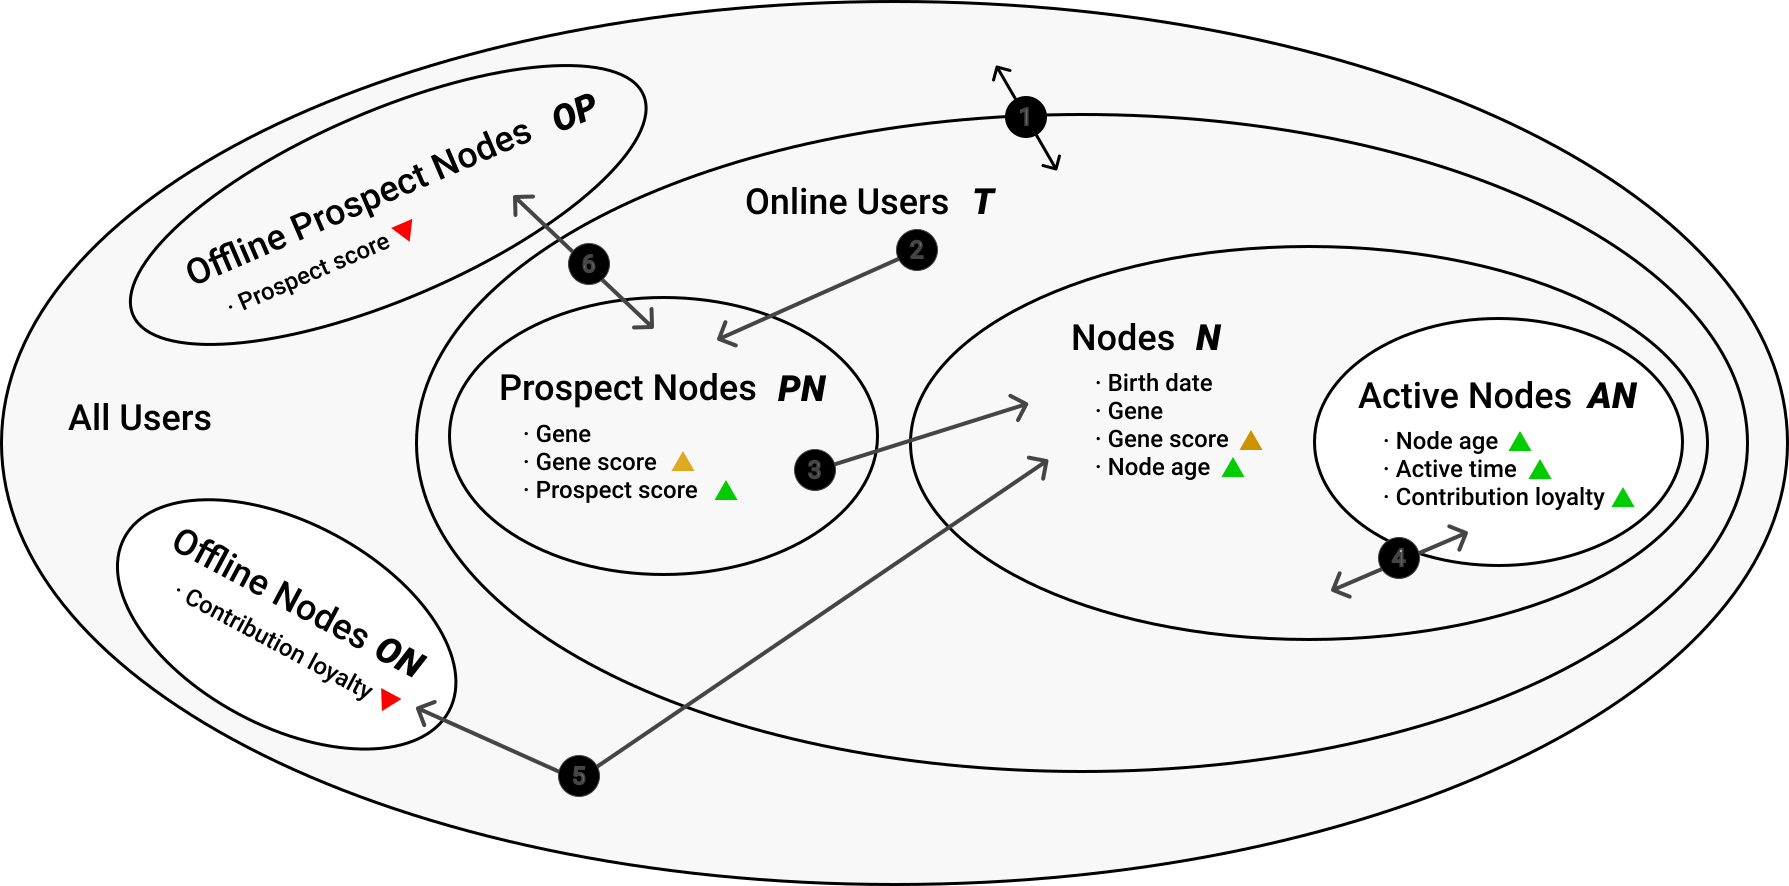
\includegraphics[width=1.05\textwidth]{fig/governance_model.pdf}
 \caption{Governance Model with actors, boundaries and variables in the Tagion system. The green triangle indicates an increase for the actor, the red triangle a decrease and the yellow an increase after an action i.e. a mating transaction.}
 \label{fig:governance_model}
\end{figure}


The boundaries are labelled with numbers in \cref{fig:governance_model} which are defined as:
\begin{enumerate}
 \item Any node can go from online to offline and vice versa. The network is open for all; it means that anyone who has not yet used the system can become a user as well. 
 
 \item Any node can become a validator-node over time and must first become a prospect node. The transition is based on a random selection, a lottery, to help ensure a broad representation of nodes. When going from a user to a prospect node or node, in general, the user is no longer anonymous, but a public servant with a public name record in the system \cref{sec:name_card_contract}.
 
 \item When a prospect nodes have been socially verified and earned enough prospect score that is being available for the network for a period of time then the prospect node becomes a node, i.e. born and receives a gene number and a birth date.
 
 \item Nodes are chosen randomly within a given interval continues to be active nodes, and active nodes are chosen randomly to be inactive nodes. Nodes and active nodes are swapped back and forth continuously to make it impossible to predict, which nodes are active in 10 minute intervals, enhancing security. A node is selected by a \abbrev{UDR}{Unpredictable Deterministic Random} algorithm, where the probability of being chosen as an active node or to continue as an active node depends on four variables:  \abbrev{gs}{Gene score},  \abbrev{at}{active time},  \abbrev{no}{node age} and \abbrev{cl}{contribution loyalty}. 
 \begin{equation}
  P_{(active)} (gs, cl, na/at)
 \end{equation}
 
 \item A node can go from online to offline and vice versa, if offline, it is not possible to be an active node or to become an active node. 
 
 \item A prospect node can go from online to offline and vice versa. 
\end{enumerate}

\subsubsection{External Node Layer} \label{sec:extenal_node_layer}
xxx

\subsubsection{Prospect Node Layer} \label{sec:prostect_node_layer}
xxx

\subsubsection{Available Node Layer} \label{sec:available_node_layer}
xxx

\subsubsection{Active Node Layer} \label{sec:active_node_layer}
xxx


\subsubsection{Reputational Scoring Model} \label{sec:reputational_scoring_model}
The model consists of actors, variables and the boundaries of the actors, including the transition over a boundary.


The variables of the actors and scoring rules for the model are defined in \cref{tab:governance_variables}.
\begin{table}[H]
 \begin{center}
  \begin{tabular}{|p{4cm}|p{8cm}|}
  \hline
  Variable name & Definition and scoring rule \\
  \hline
  Birthdate & The date a prospect node becomes a node. \\
  \hline
  Gene & A gene is unique for each node. \\
  \hline
  Gene score (Gene-diversification points) & Each time a node mates with another node, a score is calculated for them both based on how diverse their genes are compared to each other. They mate each time verification of a prospect node takes place, when an active node makes an epoch, see \cref{sec:hashgraph_cm}, and when two nodes choose to mate and validate each other. \\
  \hline
  Node age & A measure of a node's total available time for the network. Time as both a node and an active node. It increases both as a node and active node when available for the network. \\
  \hline
  Active time & Time as an active node. It increases when a node is active.\\
  \hline
  Prospect score & The Prospect score variable is a measure of how much the prospect node has been available to the network. It increases when the prospect node is available and decreases when not. \\
  \hline
  Contribution loyalty & A measure of how much the node has been active and stayed available. Non-availability of a node decreases contribution loyalty; being an active node increases loyalty. \\
  \hline
  \end{tabular}
 \end{center}
 \caption{Variables and scoring rules for the reputational scoring model}
 \label{tab:governance_variables}
\end{table}


The actors with their boundaries to each other and variables are illustrated in \cref{fig:governance_model}, the boundaries and transition over them are described below.



\subsubsection{Proof-of-People} \label{sec:proof-of-people}
The Proof-of-People protocol is a heuristic protocol with a random and social component. Heuristic, because it aims to secure the democratic principles of one person one node and that it is an actual person behind a node. One person one node cannot be accomplished, but the social component would accomplish an approximation to this. The social component makes it difficult to manage more than one node, and the scoring mechanism makes it less favourable. The approximation would ensure a highly-distributed system when it is combined with a random selection of new prospect nodes. It means no actor or a few actors would control the network when the number of nodes has a certain size, making it secure.

The protocol for becoming a node is:

\begin{enumerate}
 \item A user creates or has a name record in the system, see \cref{sec:name_card_contract}. 
 
 \item A user has a name record with an age of more than one month. The user makes a prospect node record transaction where a node-transaction fee is paid together with a staked amount. The prospect node record contains the user's public key, has the stake attached to it and is linked to the name record.
 
 \item With an average of 10 minutes, a prospect node record is chosen randomly, which burns the stake and gives a node coupon. Then the prospect node should send a proof of activity from within seven days. The proof is simply a public key to a bill in the DART, which are created within the last seven days. 
 
 \item When the user has sent the proof, two random active nodes verify the proof and give a gene to the prospect by crossing their genes with each other. The gene is added to the prospect node record and both parents sign the prospect node record. 
 
 \item \label{itm:mating_transaction} The rewarded node in the same epoch as where the coupon was issued is the first to identify the prospect in a dialogue. If the rewarded node validates the prospect, they make a mating transaction, which both signs. Both nodes receive gene score points for this transaction, and the mating transaction is linked to the prospect node's record. The gene score points are symbolised with the yellow triangle on \cref{fig:governance_model}. 
 
 \item Two semi-determined identifications should be made by two of the next ten epoch rewarded nodes. The prospect engages in a dialogue with potential validators to get two mating transactions. This is the same mating transaction as in \cref{itm:mating_transaction}.
 
 \item Now the node has received three identifications, which means it can start participating as a prospect node on the network, and receive prospect score points. When the node has reached a prospect score threshold the step is completed. 
 
 \item A second semi-determined identification of the prospect is made with two nodes from the last ten epochs from the point the prospect score is reached. This is the same mating transaction as in \cref{itm:mating_transaction}. 
 
 \item The last mating transaction creates a birth date in the prospect node record, making the prospect node a full node on the network. 
\end{enumerate}

There are three main components to the protocol:
\begin{enumerate}
 \item The first selection of prospect nodes introduces a certain time-lag by the need to have a name record with an age of one month and a stake amount. A node transaction fee ensures that small and zero transactions cannot be used to increase the chances of winning the coupon. The fee and stake ensure commitment as well.  
 \item The requirement of activity within the last seven days creates a requirement for the user to have activity in the network. 
 \item A social component that forces new nodes to engage in dialogue with other nodes, thus creating relations and communities. It is a local or virtual identification and dialogue with each other following the protocol. Both parties receive gene score points when mating, thus raising the chance for rewards to create a direct economic incentive and, indirectly, by ensuring non-evil nodes in the system, ensure the long-term sustainability and economic network worth of the system. Therefore, all nodes have a natural incentive to ensure that new nodes are real persons with honest intentions.
\end{enumerate}

A premise for the social protocol to work is that users engage in dialogue; it requires social responsibility and engagement. As long as this premise is true, the node governance components can be adjusted based on the real experience with the test network, where a balance between the work and drag of being and becoming a node compared to actual user adoption and distribution. \newline
Besides the proof-of-people protocol, a continuous evaluation of nodes can be imaged. E.g. each month, all nodes need to engage in dialogue with 3 other nodes receiving gene score points. 
More, the future perspectives of the sharding of the network would allow the network to be more local based, thus removing cultural and language barriers, which can foster people to educate each other and build a culture around the network. 

That is accomplished by a reputational scoring model and a proof-of-people protocol that is a social heuristic protocol. Both components are inspired by Charles Darwin's evolutionary theory of how species best survive in a new environment with the two main elements 1) most diversified paired genes and 2) caretaking of the offspring. These two elements are embedded in the scoring model and protocol. 

\paragraph{Defining a node} is done from democratic principles, where all can participate and where one person has one vote. These principles are translated into a permissionless system where one node has one vote, and where one person only controls one node. It would ensure full distribution of nodes because centralisation is not possible. It is not possible to ensure 100\% that one person can only control one node, but it is the aim. More, it is not required that the network is fully distributed to ensure the network is secure. The requirement is that it is distributed in a way, where many actors control an insignificant amount of nodes, thus avoiding the centralisation of power like in other networks, where few nodes may have majority control. \\
One of the downsides of democracy is that all have the same voting power independent of contribution. Thus, the Tagion system has a scoring system that values loyalty, that is, work through time, but still is open and fair for all to participate. The social component in the proof-of-people protocol tries to ensure that one person only has one node and is a real person. The protocol also selects users randomly to become nodes ensuring even distribution and fairness.  


\subsection{Economic Governance} \label{subsec:economic_governance}
The economic model of Tagion tries to stabilise the intrinsic value of the system, rather than being pegged to external currencies or assets. 
There are two main phases of economic governance, where the first is a linear and stable supply. The second phase builds on a model that aims to keep the intrinsic value of the currency stable by controlling the supply of money. 

The idea is that money reflects the underlying value of an asset; money in itself does not have value. Production in our society creates the value: the assets, which values are represented by money, make them easy to trade. Being able to represent a value for the persons using the money includes the need to trust that they can use the money elsewhere, and it needs to have a stable value over time. 
The reason a currency is trusted is that it has adoption and a stable value over time, and not because money is backed by gold or is state-backed. Adoption of the Tagion network happens over time, but the stability of the Tagion currency needs to be addressed, making it trusted. 


\subsubsection{Stable supply}
Creating a stable supply with full transparency like in Bitcoin (though decreasing supply, stable) creates trust in the system. No actor can create a significant supply and dilute the value and the trust in the system. 
Some systems have a built-in cap in the system, which needs to be changed programmatically, like Bitcoin. Tagion does not have a built-in cap, because the supply of money should somehow correspond to the adoption, and thus the representation of values in the system. Otherwise, destructive deflation in the system could cause the real use of the system to fall, because people would then tend to hold and speculate with the money instead of using it. Of course, inflation can also be destructive, but a steady and insignificant increase in the supply of money should not create hyperinflation in the system. The most important thing would be that people keep using Tagions because they trust the money and do not hold on to them due to deflation.
During the first couple of years in a monetary system's lifetime, high volatility is expected because of the low numbers of actors, which can easily both make the internal and external value go up and down because each actor's transaction can be significant in the system. As adoption occurs and the number of actors in the system becomes significant compared to a single actor, then price volatility decreases, because no single actor has a significant effect on the system. When this adoption size is reached, it leads us to the next phase, where an algorithm controlling the money supply stabilises the intrinsic value. 

\subsubsection{Stable intrinsic value}
Milton Friedman stated that ``Inflation is always and everywhere a monetary phenomenon''. This means that inflation has nothing to do with the production in society \cite{friedman_counter}. The relationship between money and the production in society can be expressed by the equation of exchange: \cite{britannica_monetarism}

\begin{equation}
 M \cdot V = P \cdot Q
 \label{eq:equation_of_exchange}
\end{equation}

\begin{itemize}
 \item[$M$]is the quantity of money. 
 \item[$V$]is the velocity of money (the number of times per year the average currency in the money supply is spent).
 \item[$P$]is the average price level of sold goods and services.
 \item[$Q$](or Y) is the real GDP for an economy.
\end{itemize}

This equation has some useful constructs of the measure of money within a monetary system, but also an external measure of GDP, which is not available for Tagion because Tagion only measures on internal variables. Tagion sees an economic system as a flow system and not as static equilibrium. The constructs in the model are used but translated into a dynamic flow model with only internal variables. A translation of the constructs to variables in the Tagion system could be: 

\begin{itemize}
 \item[$M$]is the quantity of Tagions in the system. That is a variable directly measurable in the system.  
 \item[$V$]is the number of times per year the average Tagion in the money supply is spent. It can be mapped to the variable of the number of transactions and average supply of money per year, which are direct variables in the system. 
 \item[$Q$]can be mapped with an average number of nodes in the system, which is an expression for users, and adoption in the system, thus how much of users' value the system represents. More variables, such as the acceleration of transactions, average transactions per time unit, average transaction size and acceleration can all be potential variables for the constructs in the system.
 \item[$P$]is the average price level in the Tagion monetary system, which can be expressed as: 
 \begin{equation}
  P = \frac{M \cdot V}{Q}
 \end{equation}
 The aim would be to keep the price level $P$ stable, where the only controlled variable is the supply of money, which can be regulated after a model by an algorithm. 
\end{itemize}

These variables need to be modelled, and construct-validation, correlation and causal-relation tests made. It requires a system of a particular size and much testing to model this. Tagion is confident that it is possible to keep intrinsic stability by such a model in the system. 
The aim is not an xx \% inflation target of the system, which makes no sense when external constructs as GDP are not measured, but to keep the intrinsic value in the system stable. It is accomplished by creating the adoption of the system and an intrinsic stability mechanism in the system. It should generate long-term trust and stability over time, becoming a store of value. External parties must not control the money supply and system with their interest which dilutes the trust and value of the money. 

\subsection{System Upgrade Governance}
Upgradability has been taken into consideration on two main levels: Node Software, which concerns the actual base protocols for running a node, and Script Function Upgrades, which concerns the function scripts in the network. All scripts are stored in the DART, meaning it does not require an upgrade of the base protocols, but just a change of the script function state in the DART. Function scripts are node governance and economic governance algorithms.

\subsubsection{Node Base Protocol Upgrade}
The upgrade of the node base protocols should be backwards compatible with the previous version. It means the software can run the current network version and the new one, but it does not mean the networks are compatible, which can be divided into two categories minor and core upgrades:

\paragraph{Minor and bug-fixes upgrades}
This upgrade does not change the structure of the database and core algorithms, meaning that it can run in the same network as the current. It requires 5/6 of the active nodes to approve the upgrade. 
\paragraph{Core and structural upgrades}
Core and structural upgrades make hard changes, which can be core algorithms for cryptography or the structure of the database, which make the current network incompatible with the new one. It means that the nodes approving the new network operate both the current and new network in parallel until the upgrade is approved. It requires a 5/6 majority of the active nodes to approve the upgrade and to enforce the new network version. 
\paragraph{Script Function Upgrades}
Script function upgrades are when a script in the database in the network is changed, created or deleted. It does not require the installation of a new binary on the computer the node is running on. Before a new function is approved, 5/6 of the active nodes need to approve it.

\subsection{Common Resources} \label{sec:common_resources}
The Tagion network is a common resource, meaning that no state or private entity should own it because it serves a common purpose for the whole community and the users of the system. 

The resources are the actual network, and the governance mechanism all the IP (intellectual property) related to Tagion, which is listed below.

\subsubsection{Open Source code}
The source code is released under a GNU GPL or similar license and owned by the Tagion Foundation. The licensing is in process. Closed or commercial projects do need permission to use the source code.
At the moment the git repository is not opened. Preparations to open the repository are being made.
Before the open-source license is defined, and the open patent license has been given to the Tagion Foundation from I25S ApS, the repository cannot be opened. It is planned to open the project as soon as possible. People with legitimate reasons to verify the code can write to info@tagion.org and a copy of the source code can be shared after a signed NDA is in place.

\subsubsection{Patents}
EU patents are filed in the company name I25S ApS. The patents concern 1) a database system and 2) a network gossip protocol.
The database system, which is implemented as the DART in Tagion, is a distributed database system that can efficiently search and store data based on a cryptographic hash enabling the network to execute transactions in parallel thus promoting performance and scalability.
The gossip protocol is an efficient way to share information among all members of the network.

\paragraph{Open Licenses}
An open license is defined to be a free patent license given to the open-source project that cannot be revoked.
All open-source projects having the same type of license as the Tagion Project are as a rule of thumb granted a free license that cannot be revoked automatically.
Other open-source projects need to apply for an open license. The licenses cannot be revoked when first given.
The Tagion Foundation and project is given an open license by I25S. Projects that fork the Tagion code need an open license by default.

\subsubsection{“Tagion” Trademark}
An EU Trademark is registered for “Tagion” and owned by the Tagion Foundation including related internet domains. 
The reason for the trademark is to make sure that projects, which are forking the source and governance model, cannot call themselves Tagion XYC. It confuses the end-users and community, thus multiple projects with similar names should be avoided.
Tagion can protect itself from other projects or entities that wish to associate themselves with Tagion for malicious purposes.



\section{Introduction}

This document describes the Tagion core network.\\
The tagion core network includes the byzantine consensus algorithm, the consensus database and description of node validators and the basic node selections. 

\subsection{Network Architecture}
The Tagion network architecture consist of a collections of computer nodes which are able to send messages between each other (A \bfit{computer node} is named \bfit{node} in this document). Each node can send a message to any other node in the network.\\
The nodes in the network has different roles and the nodes will change roles over the lifetime depended controlled by the Tagion consensus rule.\\ 

The node roles are:
\begin{itemize}
	\item[\bfit{Active Node}] The node in this role category takes care of the validations.
	\item[\bfit{Standby Node}] Those nodes are waiting to be selected  as validators.
	\item[\bfit{Swap Node}] Those nodes has been selected to be swapped with an \bfit{Active Node} and become a validator.  
	\item[\bfit{Prospect Node}] Nodes in this category are waiting to become and 'real' node in the network 
	\label{tab:node_roles}
\end{itemize}

All the nodes communicates via protocol call libp2p \cite{libp2p}. The role of the node actors are selected randomly (\bfit{UDR} \cref{sec:SMT}) according to the node consensus selection rules \cref{sec:mutation}.

\begin{figure}[H]
	\centering
	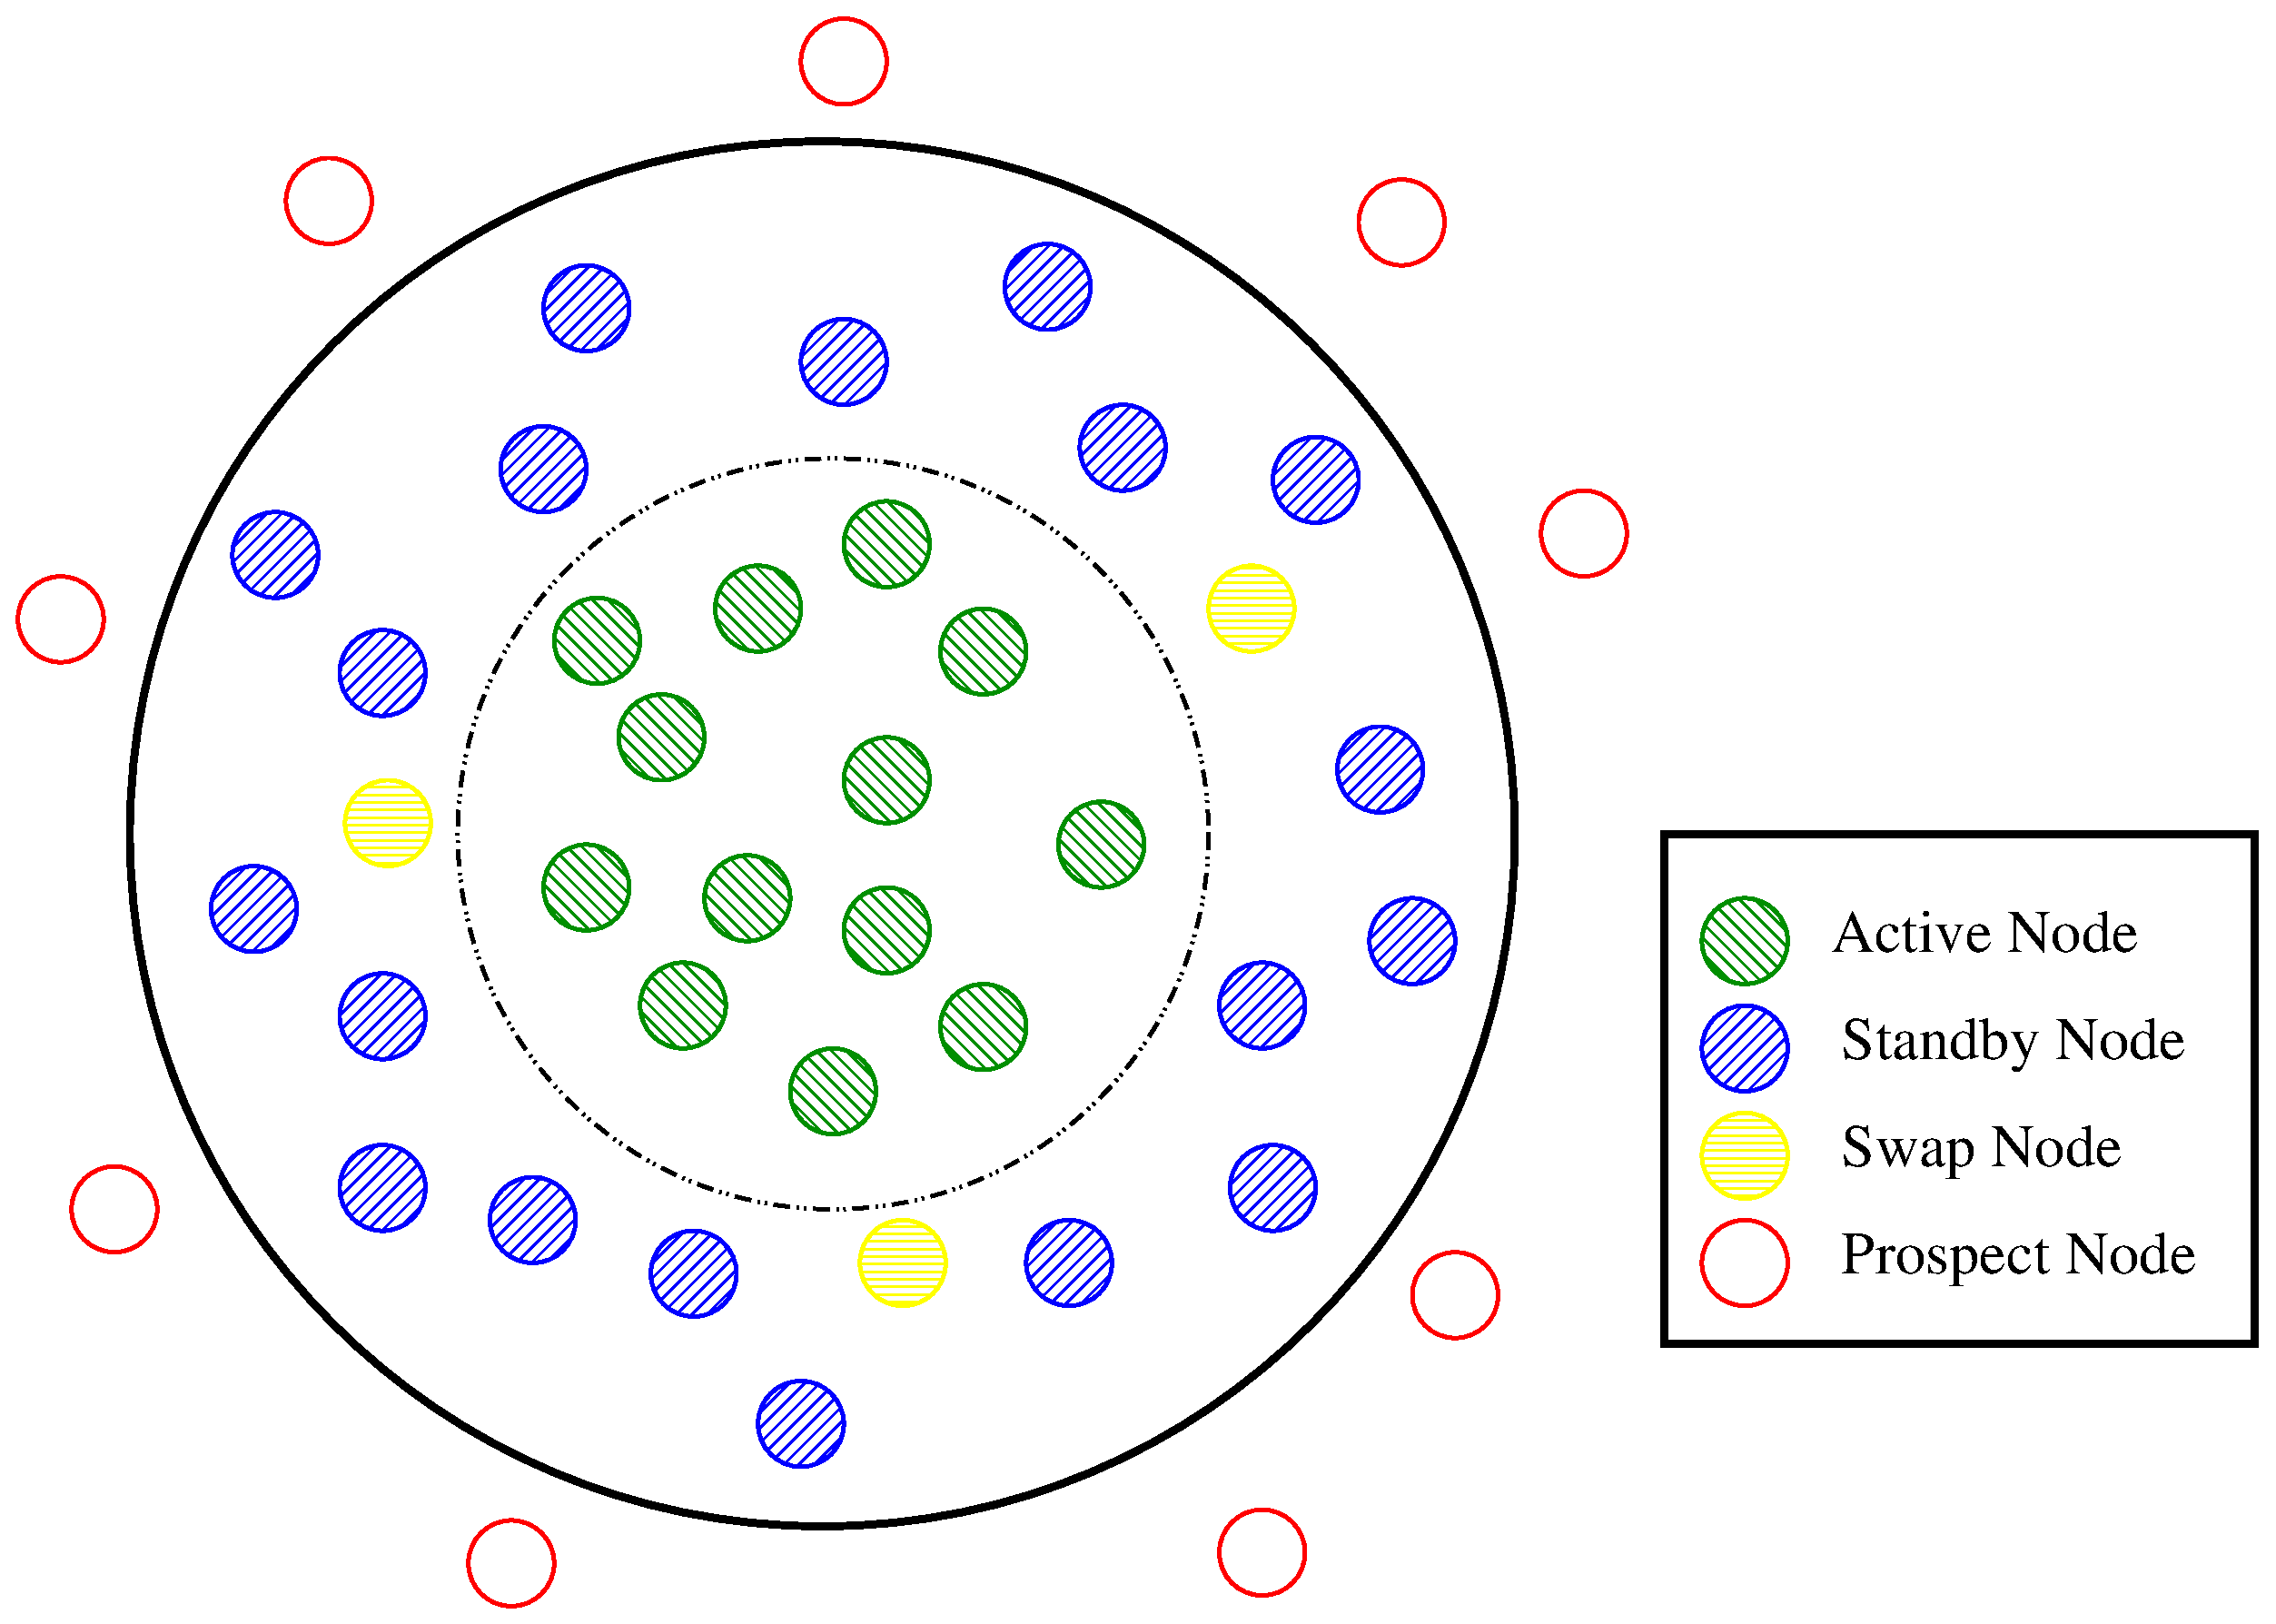
\includegraphics[width=0.8\textwidth]{fig/network_architecture.eps}
	% dart_bw.eps: 17766x12625 px, 300dpi, 150.42x106.89 cm, bb=0 0 4264 3030
	\caption{The Network Architecture}

	\label{fig:network_architecture}
\end{figure}

The \bfit{Active Node}'s validates the transaction and used the Hashgraph algorithm \cref{sec:hashgraph_cm} to reach consensus. The Hashgraph algorithm is capable of producing a consensus order list of transaction (Defined as \bfit{transaction list}). This means that all the \bfit{Active Node}'s will produces the same order of transactions.\\
The transaction list is processed in that order the procedure for execution can be found in \cref{sec:network}.
 
\subsection{Node Architecture}
The node core program is implemented in the programming language D with some C and Go libraries for crypto, network and virtual engine functions. It is structured, as shown in the figure below. 

\begin{table}[H]
	{%
		\newcommand{\mc}[2]{\multicolumn{#1}{#2}}
		\begin{center}
			\begin{tabular}{|c|c|}
				\hline
				\mc{2}{|c|}{HiRPC (HiBON) Dataformat for communication}\\
				\hline
				\mc{2}{|c|}{NODE}\\
				\hline
				User API - TLS 1.2 & P2P Network\\
				\hline
				\mc{2}{|c|}{Tagion Virtual Machine}\\
				\hline
				\mc{2}{|c|}{Consensus mechanism : Hashgraph}\\
				\hline
				\mc{2}{|c|}{Storage : Distributed Database DART }\\
				\hline
				\mc{2}{|c|}{Blockchain : Epoch Records} \\
				\hline
			\end{tabular}
		\end{center}
	}%
	\caption{Tagion Node stack}
	\label{tab:node_stack}
\end{table}


A Tagion Node is divided into units as shown in \cref{fig:node_service} and each unit handles a service function in the following manner:

A smart-contract is sent to the Transaction-service-unit which are fetching the inputs date form the distributed Data-base DART unit (see \cref{sec:DART}) and verifying their signatures of the inputs. The DART-unit connects to other DARTs via the P2P-unit. The transaction-unit forwards the smart-contract to the Coordinator-unit and this unit that is gossiped to the network via the P2P-unit.\\
When the Coordinator receives an event with a smart-contract, the smart-contract contract is verified and executed via the \abbrev{TVM}{Tagion Virtual Machine} unit, and the results of the outputs are verified.\\
The Coordinator adds it to an event in the Hashgraph and gossips the informations via the P2P-unit to other nodes in the network.    
When the Coordinator finds an epoch, it make a list of ordered transactions and forwards this list to the Transcript-service-unit. The transcript-unit executes the smart-contracts in order and produces list called an Recorder. A Recorder is contains list of all the inputs to be erased and all the outputs to be added. The Coordinator send Recorder to the DART-uint which executes this list. The DART-unit forwards the Recorder to the Recorder-unit and the Recorder adds this to a block-chain.\\
In the case that the Coordinator resolves that super majority of the active-nodes dose not agree the Coordinator send an undo-instruction to the Recorder-unit.\\
If the Recorder-unit receives an undo-instruction the recorder will send the Recorder-list in reverse order to the DART-unit and the DART-unit will perform this action and put the DART in the previous state before the last Epoch.
The Logger-unit and the Monitor-unit used for debugging and monitoring the network.

\begin{figure}[H]
	\centering
	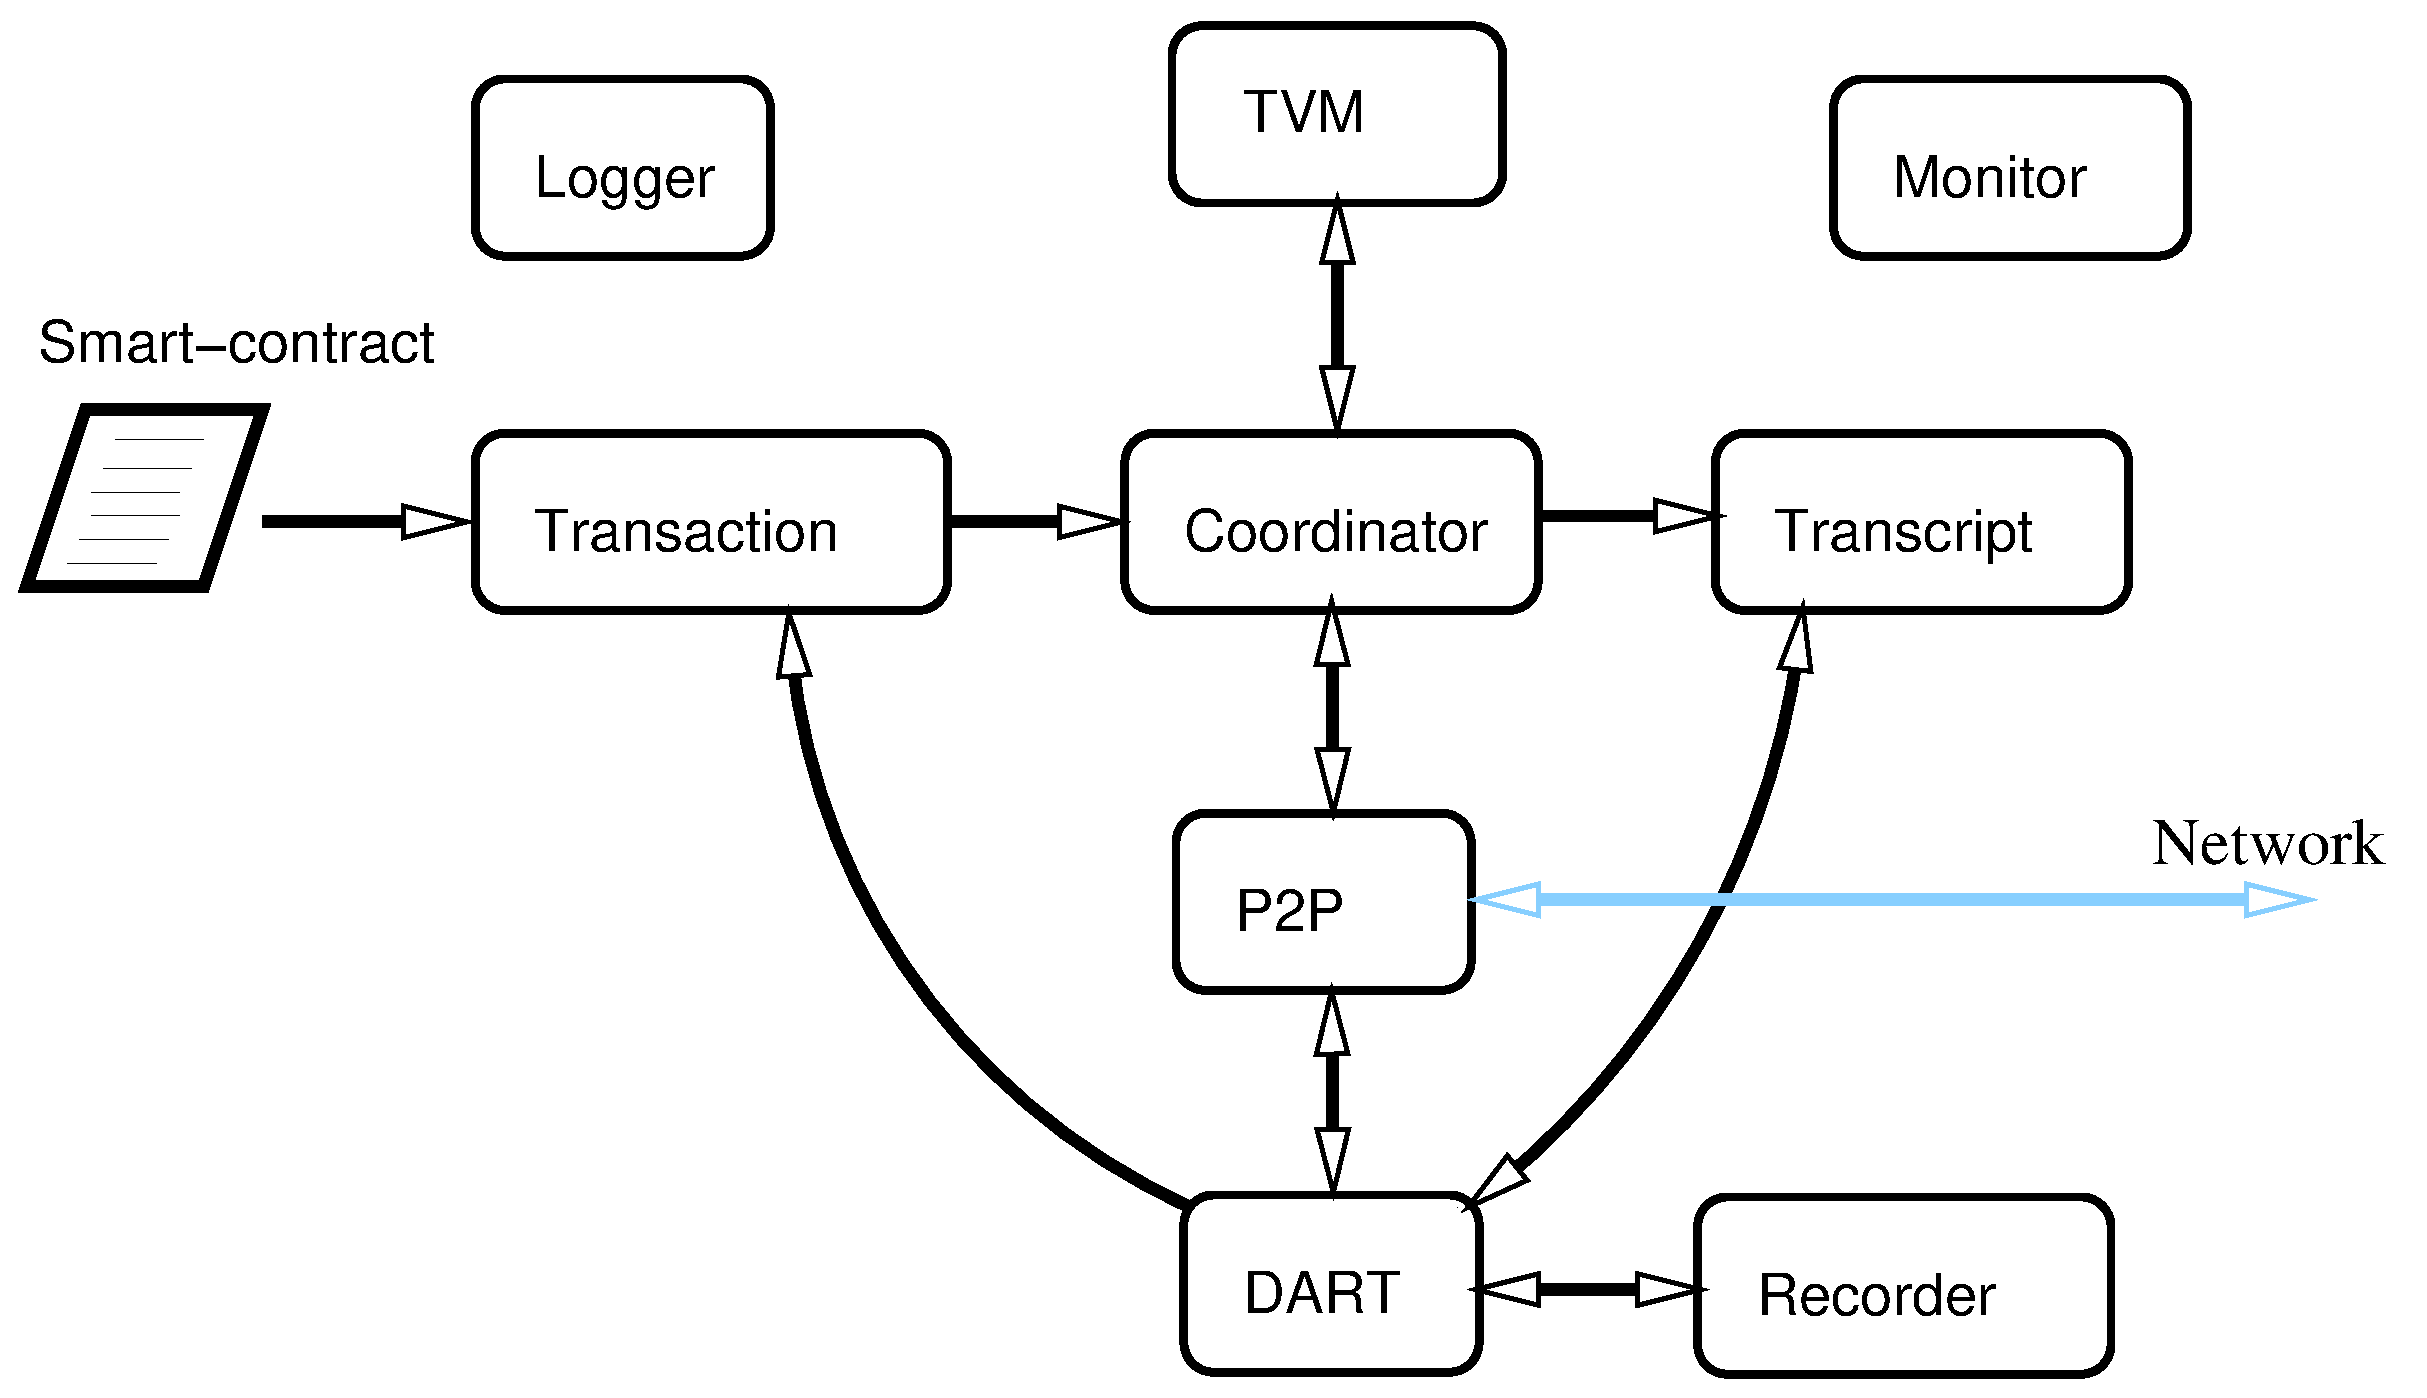
\includegraphics[width=0.8\textwidth]{fig/node_service.eps}
	% dart_bw.eps: 17766x12625 px, 300dpi, 150.42x106.89 cm, bb=0 0 4264 3030
	\caption{The Tagion Node Architure}
	\label{fig:node_service}
\end{figure}


Each of the services is running as independent tasks and communication between each-other via commutation channels. The different services modules perform the service as described in the list below.

\begin{itemize}
	\item[\bfit{Coordinator}] This service manages the hashgraph-consensus and controls other related service for the node. 
	The Coordinator generates and receives events and relays to the network. This service also generates the epoch and sends the information to the ScriptingEngine services.
	\item[\bfit{Transaction}] This service receives the incoming transaction script, validates, verifies and fetches the data from the DART and sends the information to the Coordinator.
	\item[\bfit{DART}] Services to the Distributed-database
	\item[\bfit{P2P}] This service handles the peer-to-peer communication protocol used to communicate between the nodes
	\item[\bfit{TVM}] Handles the executions of the smart contracts
	\item[\bfit{Transcript}] Services the Epoch and orders the script execution
	\item[\bfit{Recorder}] This services recorder this history of the DART.
	\item[\bfit{Logger}] The service handles information logging for the different services
	\item[\bfit{Monitor}] The Monitor service is used to graphical monitor the activities locally via a web interface.
\end{itemize}


Estimated bandwidth requirement and the average propagation for a transaction the formulas in \cref{sec:gossip_model}.
 
From simple experimental model result.\\

Example for a network with nodes $N=11$ an event size of $E_{size}=500bytes$ and network delay of $t_{net}=300ms$ the estimated epoch propagation delay
and the bandwidth of:
\begin{align*}
n_{round} &= 2.2 \cdot ln(11) &\approx  5.27\\
t_{epoch} &= 3.5 \cdot n_{round} \cdot 300ms & \approx 5.5s \\
B &= 500bytes \cdot 11^2 &= 60500bytes \\
BW &= 8 \cdot B / (n_{round}\cdot 300ms) &\approx 28kbit/s \\
\end{align*}
And with $N=31$:
\begin{align*}
n_{round} &= 2.2 \cdot ln(31) & \approx  8.6\\
t_{epoch} &= 3.5 \cdot n_{round} \cdot 300ms & \approx 8s \\
B &= 500bytes \cdot 101^2 & \approx 481kbytes \\
BW &= 8 \cdot B / (n_{round}\cdot 300ms) &\approx 152kbit/s \\
\end{align*}
And with $N=101$:
\begin{align*}
n_{round} &= 2.2 \cdot ln(101) & \approx  10.15\\
t_{epoch} &= 3.5 \cdot n_{round} \cdot 300ms & \approx 10.6s \\
B &= 500bytes \cdot 101^2 & \approx 5.1Mbytes \\
BW &= 8 \cdot B / (n_{round}\cdot 300ms) &\approx 1.2Mbit/s \\
\end{align*}
And with $N=1001$:
\begin{align*}
n_{round} &= 2.2 \cdot ln(11) & \approx  15\\
t_{epoch} &= 3.5 \cdot n_{round} \cdot 300ms & \approx 16s \\
B &= 500bytes \cdot 1001^2 & 501Mbytes \\
BW &= 8 \cdot B / (n_{round}\cdot 300ms) &\approx 80Mbit/s \\
\end{align*}

In this example the epoch delay increases round 5s when $N$ is increased by a decade and the bandwidth requirement is increased around 50 times or more.



\pagebreak
\section{Hashgraph Consensus Mechanism} \label{sec:hashgraph_cm}
The Tagion network is based around a Hashgraph consensus algorithm and mathematical proof discovered by Leemon Baird \cite{SWIRLDS_HASHGRAPH}. This algorithm solves the Byzantine Generals’ Problem of generating a consensus order list of actions between distributed computer nodes connected in a network.
If more than 2/3 of the nodes follows the same consensus rules, all the nodes will, in finite time, reach the same order of events.
The network distributes the information via a gossip protocol, sending information about the data received from the other nodes in the network. All the nodes solving the Hashgraph algorithm will come to the same order of transactions.
Figure 1 below shows a Hashgraph of gossip information representing the information flow between network nodes. In finite time all nodes in the network will be able to build the same Hashgraph of gossip information.


\begin{figure}[ht]
 \centering
 % Replace this when we get the wavefront in
 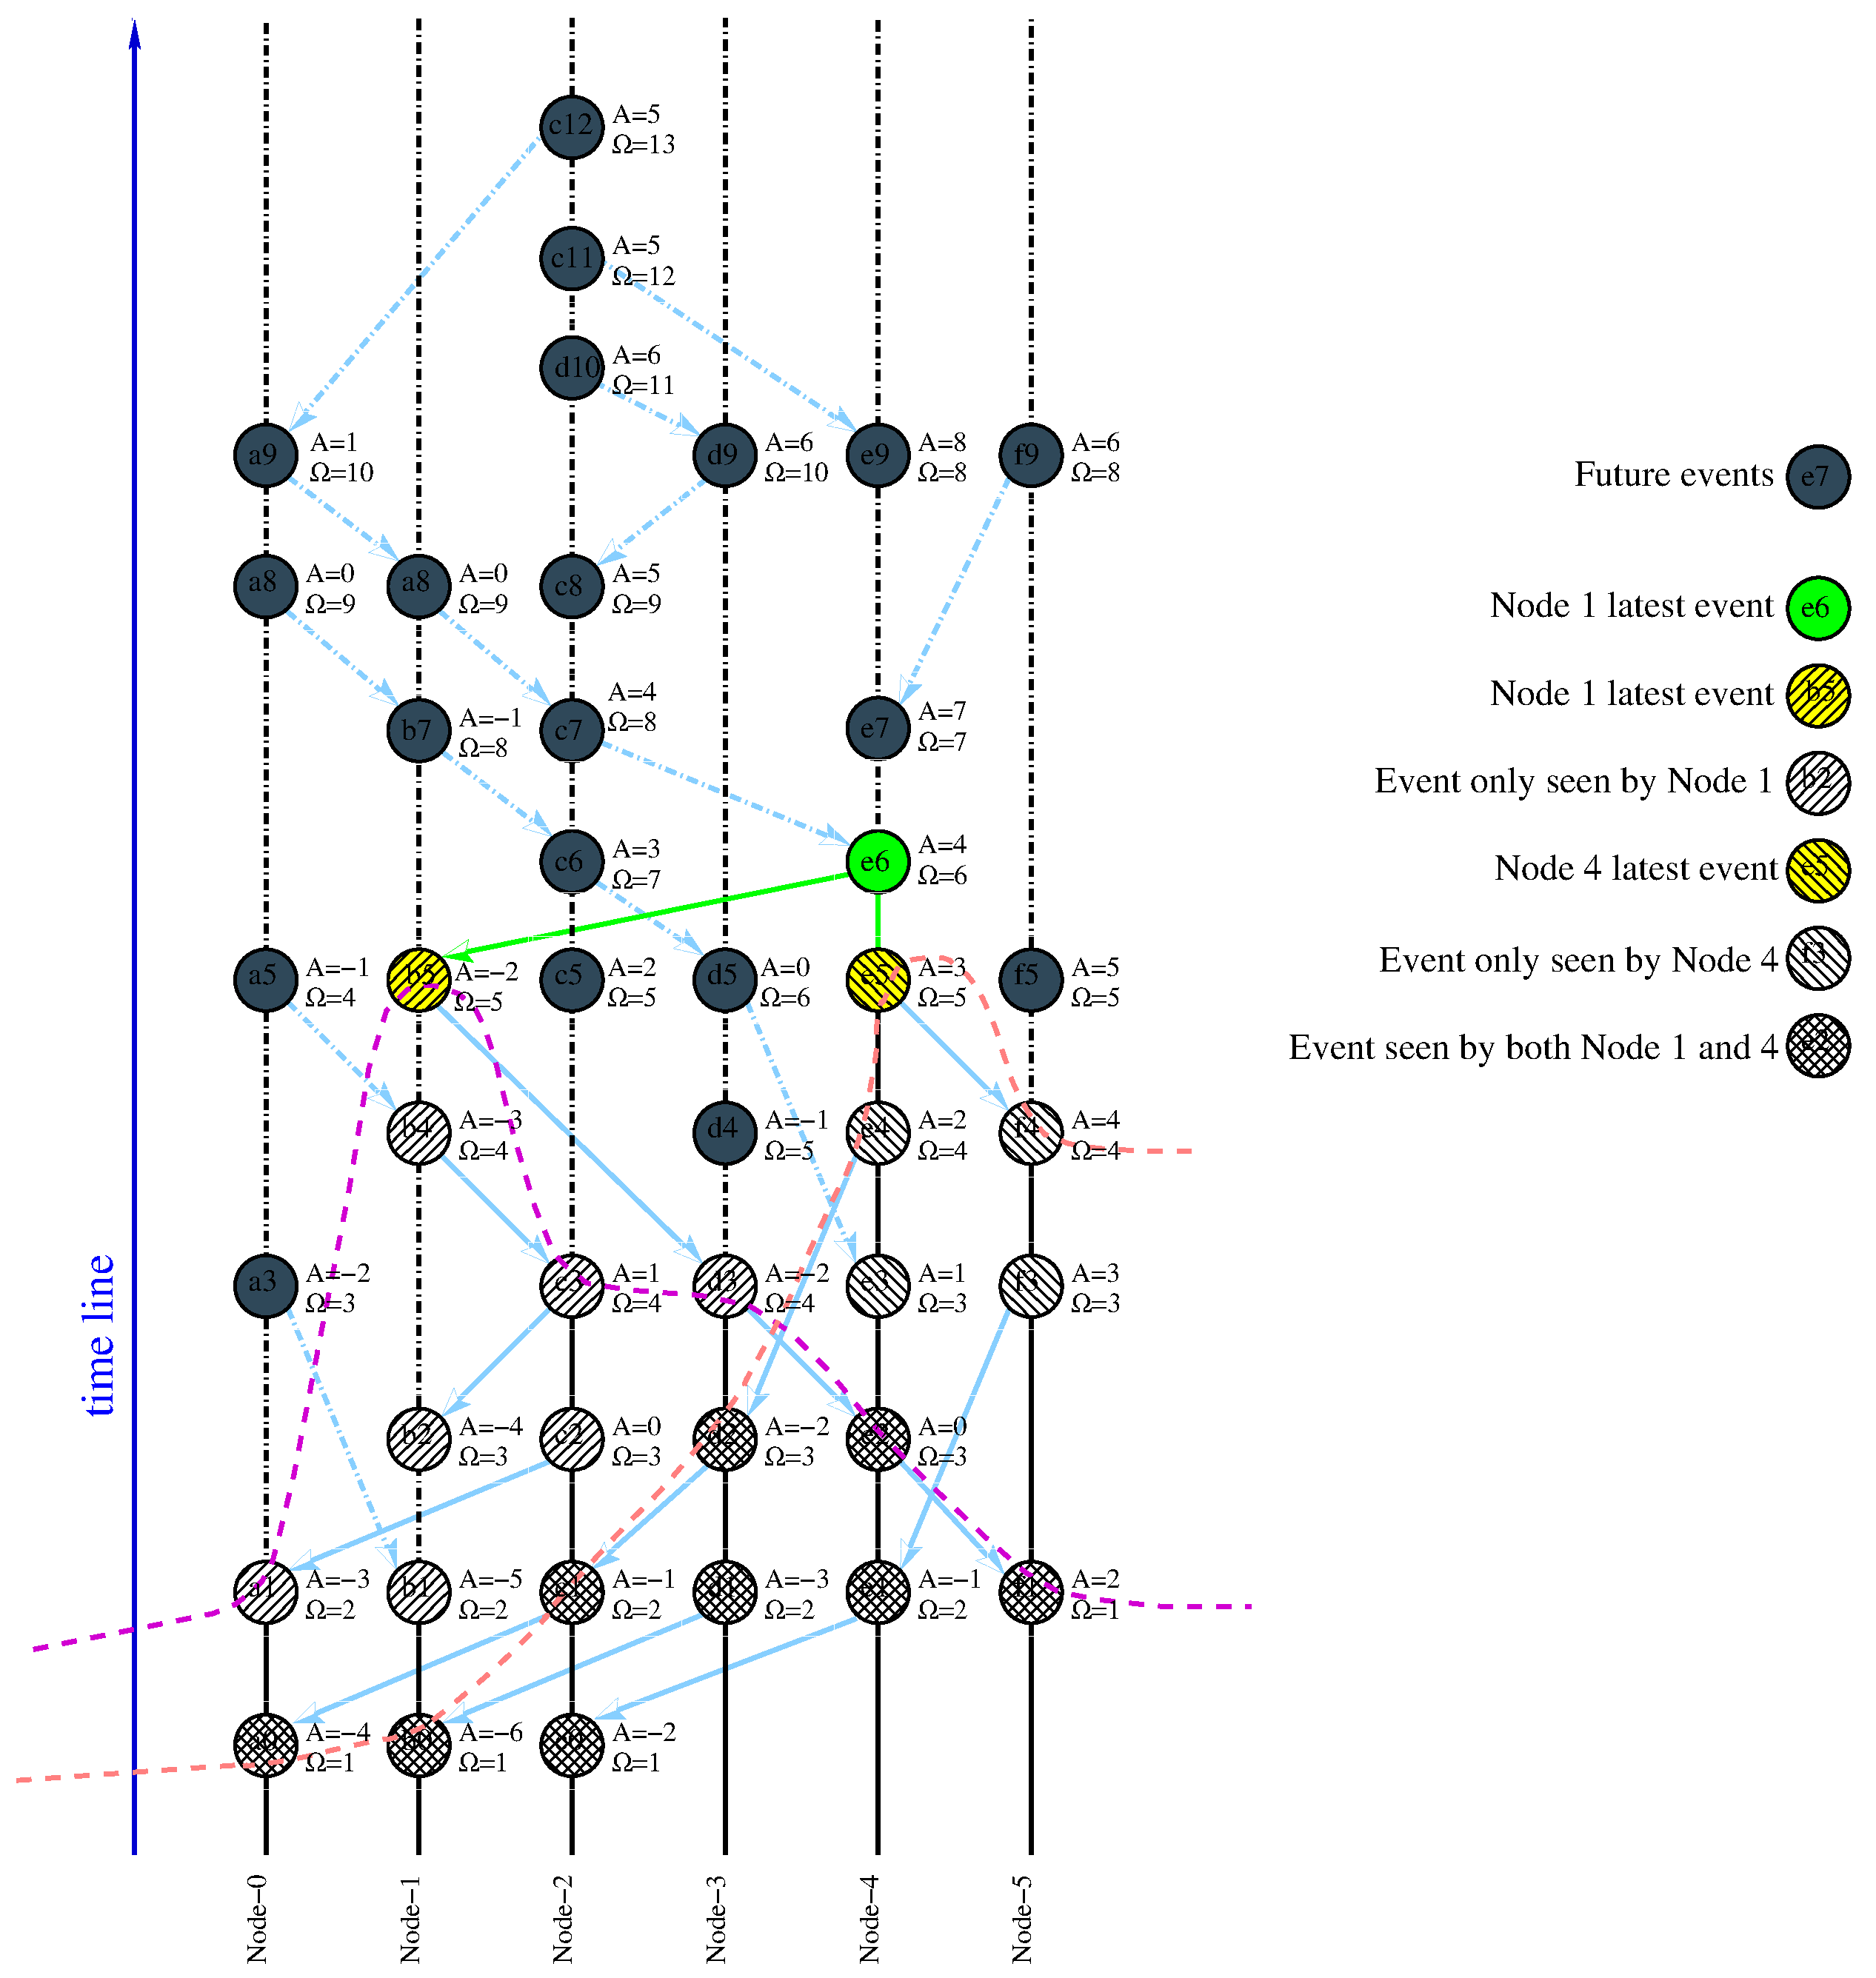
\includegraphics[width=0.7\textwidth]{fig/wavefront_and_order_long.eps}
% 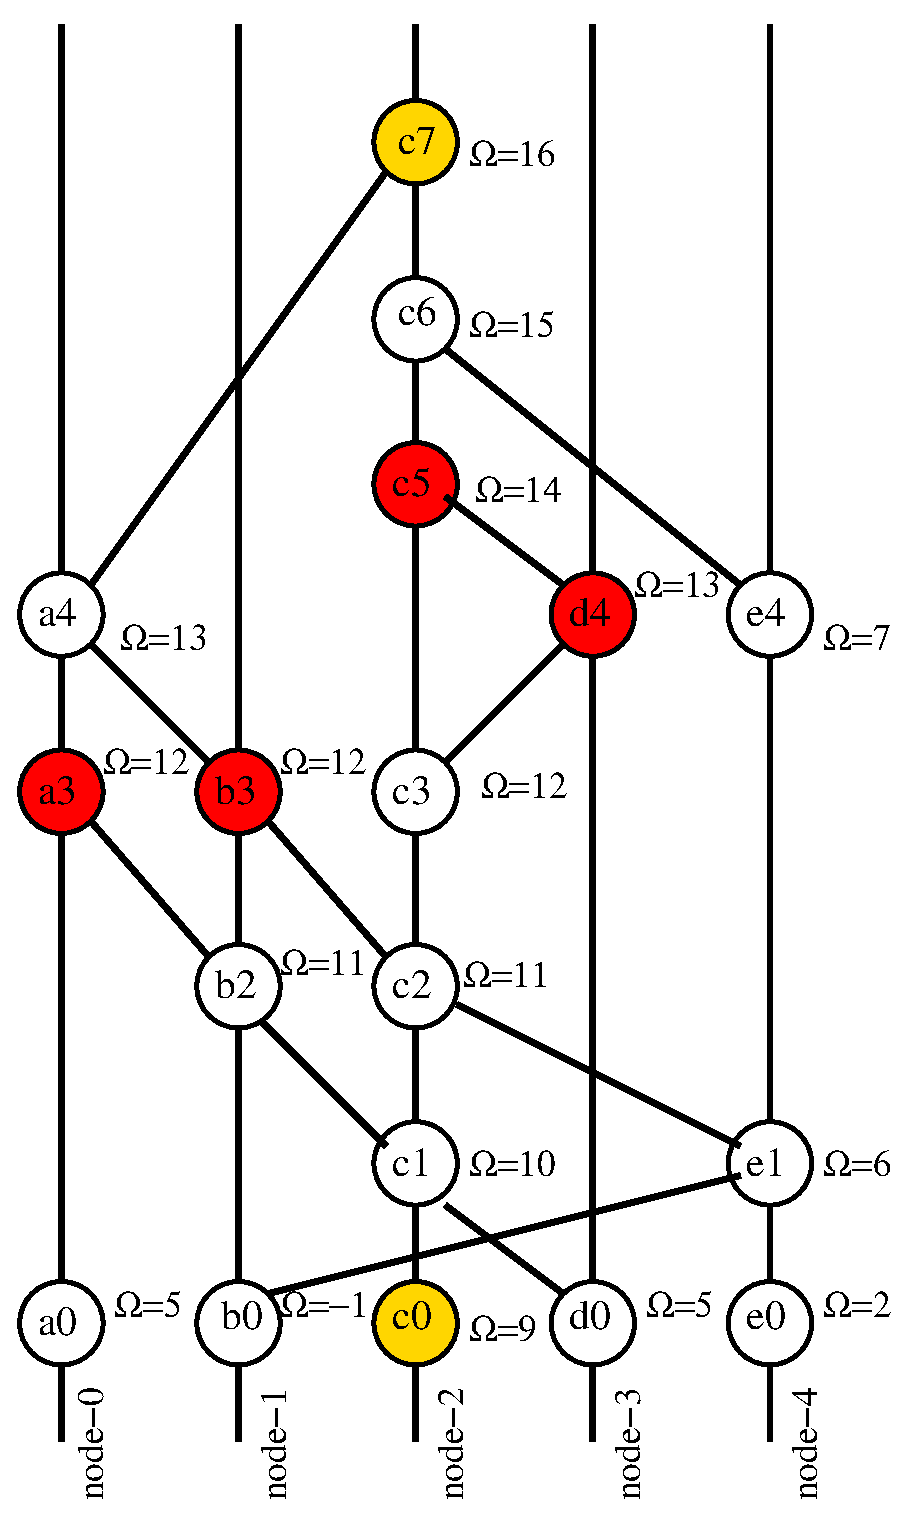
\includegraphics[width=0.45\textwidth]{fig/wavefront_and_order_small_no_alt.eps}
 % wavefront_and_order.eps: 3358x4625 px, 300dpi, 28.43x39.16 cm, bb=0 0 806 1110
 %\caption{Hashgraph with altitude(A) and parameter $\Omega$}
 \caption{Hashgraph with parameter $\Omega$}
 \label{fig:wavefront}
\end{figure}

% Hashgraph with altitude (A) order parameter Ω is shown. 
Each vertical line represents a compute node and each circle an event. The line between the events represents the communication of the events between the nodes. 
The events coloured red define a witness that is used to divide the consensus into rounds. Each round decides a list of events to be collected. This list of events is called an epoch and must be sorted into the same order as all other nodes. The description of the Hashgraph algorithm can be found in \cite{SWIRLDS_HASHGRAPH}.

% We take this out for now because of patent issues
\pagebreak

\subsection{Gossip protocol and Wavefront propagation}
The Hashgraph algorithm uses a gossip protocol called “gossip about gossip” to propagate information between the nodes. It means node A sends all the information of the communication that it knows to a randomly selected node B. This enables node B to construct the same Hashgraph as node A.

In the Tagion network, a protocol called Wavefront is used to exchange information between two nodes, ensuring that node A and B only need to communicate three times to share the state of the graph.
Each node keeps track of an integer value called Altitude. Altitude is increased by one for each event created by the node. Each node stores its current view of Altitude for each node in the network.
By exchanging information about the Altitude between two nodes, both can figure out if their Wavefront is higher and send a list of events which are in front.
The Wavefront information exchange has four states:

\begin{enumerate}
 \item 
 Node A selects random Node B and sends a list of all Altitudes. This state is called a tidal-wave.
 \item 
 Node B receives a tidal-wave from Node A. If Node B has already sent a tide-wave to Node A, then Node B will send what is called a breaking-wave to Node A. Otherwise Node B will return a list of all events which are in front of the tidal-wave of Node A. This state is called first-wave.
 \item 
 If Node A receives a first-wave from Node B, it returns a list of all the events which are in front of Node B. When this state has been reached the wavefront exchange ends.
 \item 
 If Node A or Node B receives a breaking-wave, the wavefront communication is dropped. This prevents both nodes from going into an infinity echo where they forever send information back and forth.
In the network, a node will often have many simultaneous wavefront connections so it will sometimes receive the same event package from other nodes. Then it will drop any duplicated events it receives.  
\end{enumerate}



\pagebreak

\subsection{Consensus Ordering}\label{sec:consensus_ordering}
In the Tagion implementation of the Hashgraph algorithm, an Event is only allowed to point to one or none ``other parent'' which is called a ``father-event'' as shown om \cref{fig:consensus_order}. This strategy aids in solving the graph forking problem and simplifies the consensus ordering.
The ``self-parent'' is defined as a ``mother-event'' in the Tagion implementation. An event must have a mother-event but doesn't have to have a father-event.

Each event points to the previous event called the mother-event, and some also point to another father-event. The mother-event is defined as the previous event from the same node. The father is an event sent via the gossip network from another node. 

The order $\Omega$ is calculated as:
\begin{equation}
 \Omega_{B,k+1} = max \big(\Omega_{A,k} , \Omega_{B,k} \big) +1
\end{equation}

The events in an epoch list are sorted by the order $\Omega$. According to \cref{equ:order} which define if an event A must be ordered before a B event. If the order of two events is equal, then the nested function $l'$ \cref{equ:nested_order} is use to decided the order.\\
A event is defined to be fatherless if the lineage of an event don't have a father back to the Eva event, and an Eva-event is defined to be an event without a mother and/or a father.
The following expression is used to order the events:

\begin{align}
 {l}(A,B) & = 
    \begin{cases}
         {l'}(A,B) &  	\text{if}  ~ ({\Omega}_{A} = {\Omega}_{B} )  \\ 
        {{\Omega}_{A} < {\Omega}_{B}} & 
        \text{otherwise}
    \end{cases} 
    \label{equ:order}    
\end{align}

\begin{align}
{l'}(A,B) & = 
\begin{cases}
{l}(A_{father},B_{father}) &  	
\text{if}  ~ (\text{A has a father} ~ \&  ~ \text{B has a father}) \\ 
{l}(A_{father},B_{mother}) &  	
\text{if}  ~ (\text{A has a father} ~ \&  ~ \text{B has a mother}) \\ 
{l}(A_{mother},B_{father}) &  	
\text{if}  ~ (\text{A has a mother} ~ \&  ~ \text{B has a father}) \\ 
{l}(A_{mother},B_{mother}) &  	
\text{if}  ~ (\text{A is not fatherless} ~ \&  ~ \text{B is not fatherless}) \\ 
0 &  	
\text{if}  ~ (\text{A is not fatherless}) \\ 
1 &  	
\text{if}  ~ (\text{B is not fatherless}) \\ 
{h}_{A} < {h}_{B} & 
\text{otherwise (Only happens for none orderd event)}
\end{cases} 
\label{equ:nested_order}    
\end{align}
If parameter $l(A,B)$ is $'true'$ if event A is ordered before event B (see \cref{sec:order_function}).

Note. An event which are fatherless is not allowed to contain a payload and an node must have participated in producing one epoch before the payload can be considered valid. 

\begin{figure}[H]
 \centering
 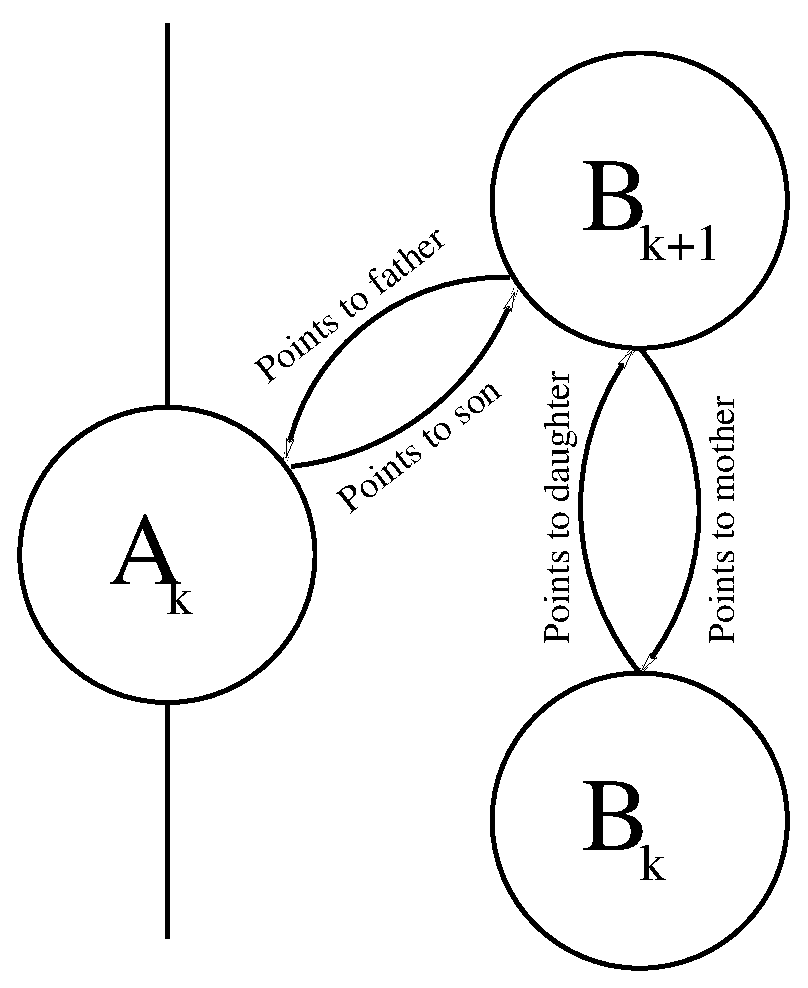
\includegraphics[width=0.5\textwidth]{fig/consensus_order.eps}
 % consensus_order.eps: 1550x1908 px, 300dpi, 13.12x16.15 cm, bb=0 0 372 458
 \caption{Events and relations}
 \label{fig:consensus_order}
\end{figure}



\pagebreak
\section{Distributed Database (DART)}\label{sec:DART}

\abbrev{DART}{Distributed Archive of Random Transactions} [Patent \cite{dart_patent}]
 is built to store and keep track of transactions in the Tagion network. The database efficiently handles the removal and addition of transactions in a secure and distributed manner.
Each transaction is stored in a distributed hash-table using a cryptographic hash of the transaction T data. Each transaction is identified by a unique hash value h. The transaction is put into a table ordered by the numerical value of the hash.
\begin{equation}
 h = H(T), ~ h \in [0:2^{N-1}-1], ~ N \in \mathbb{N}
\end{equation}

\begin{equation}
  S_i \in [i \cdot 2^{N-M}:(i+1) \cdot 2^{N-M}], ~ i \in [0:m-1], ~ m = 2^M
\end{equation}


\begin{itemize}
 \item[$H$] is the cryptography hash function
 \item[$N$] represents the number of bits
 \item[$M$] represents the bit witdh of the sector
 \item[$h$]  hash value
 \item[$S$]  is sections
 \item[$m$]  hash-table divided into sections $S$
\end{itemize}

\begin{figure}[H]
 \centering
 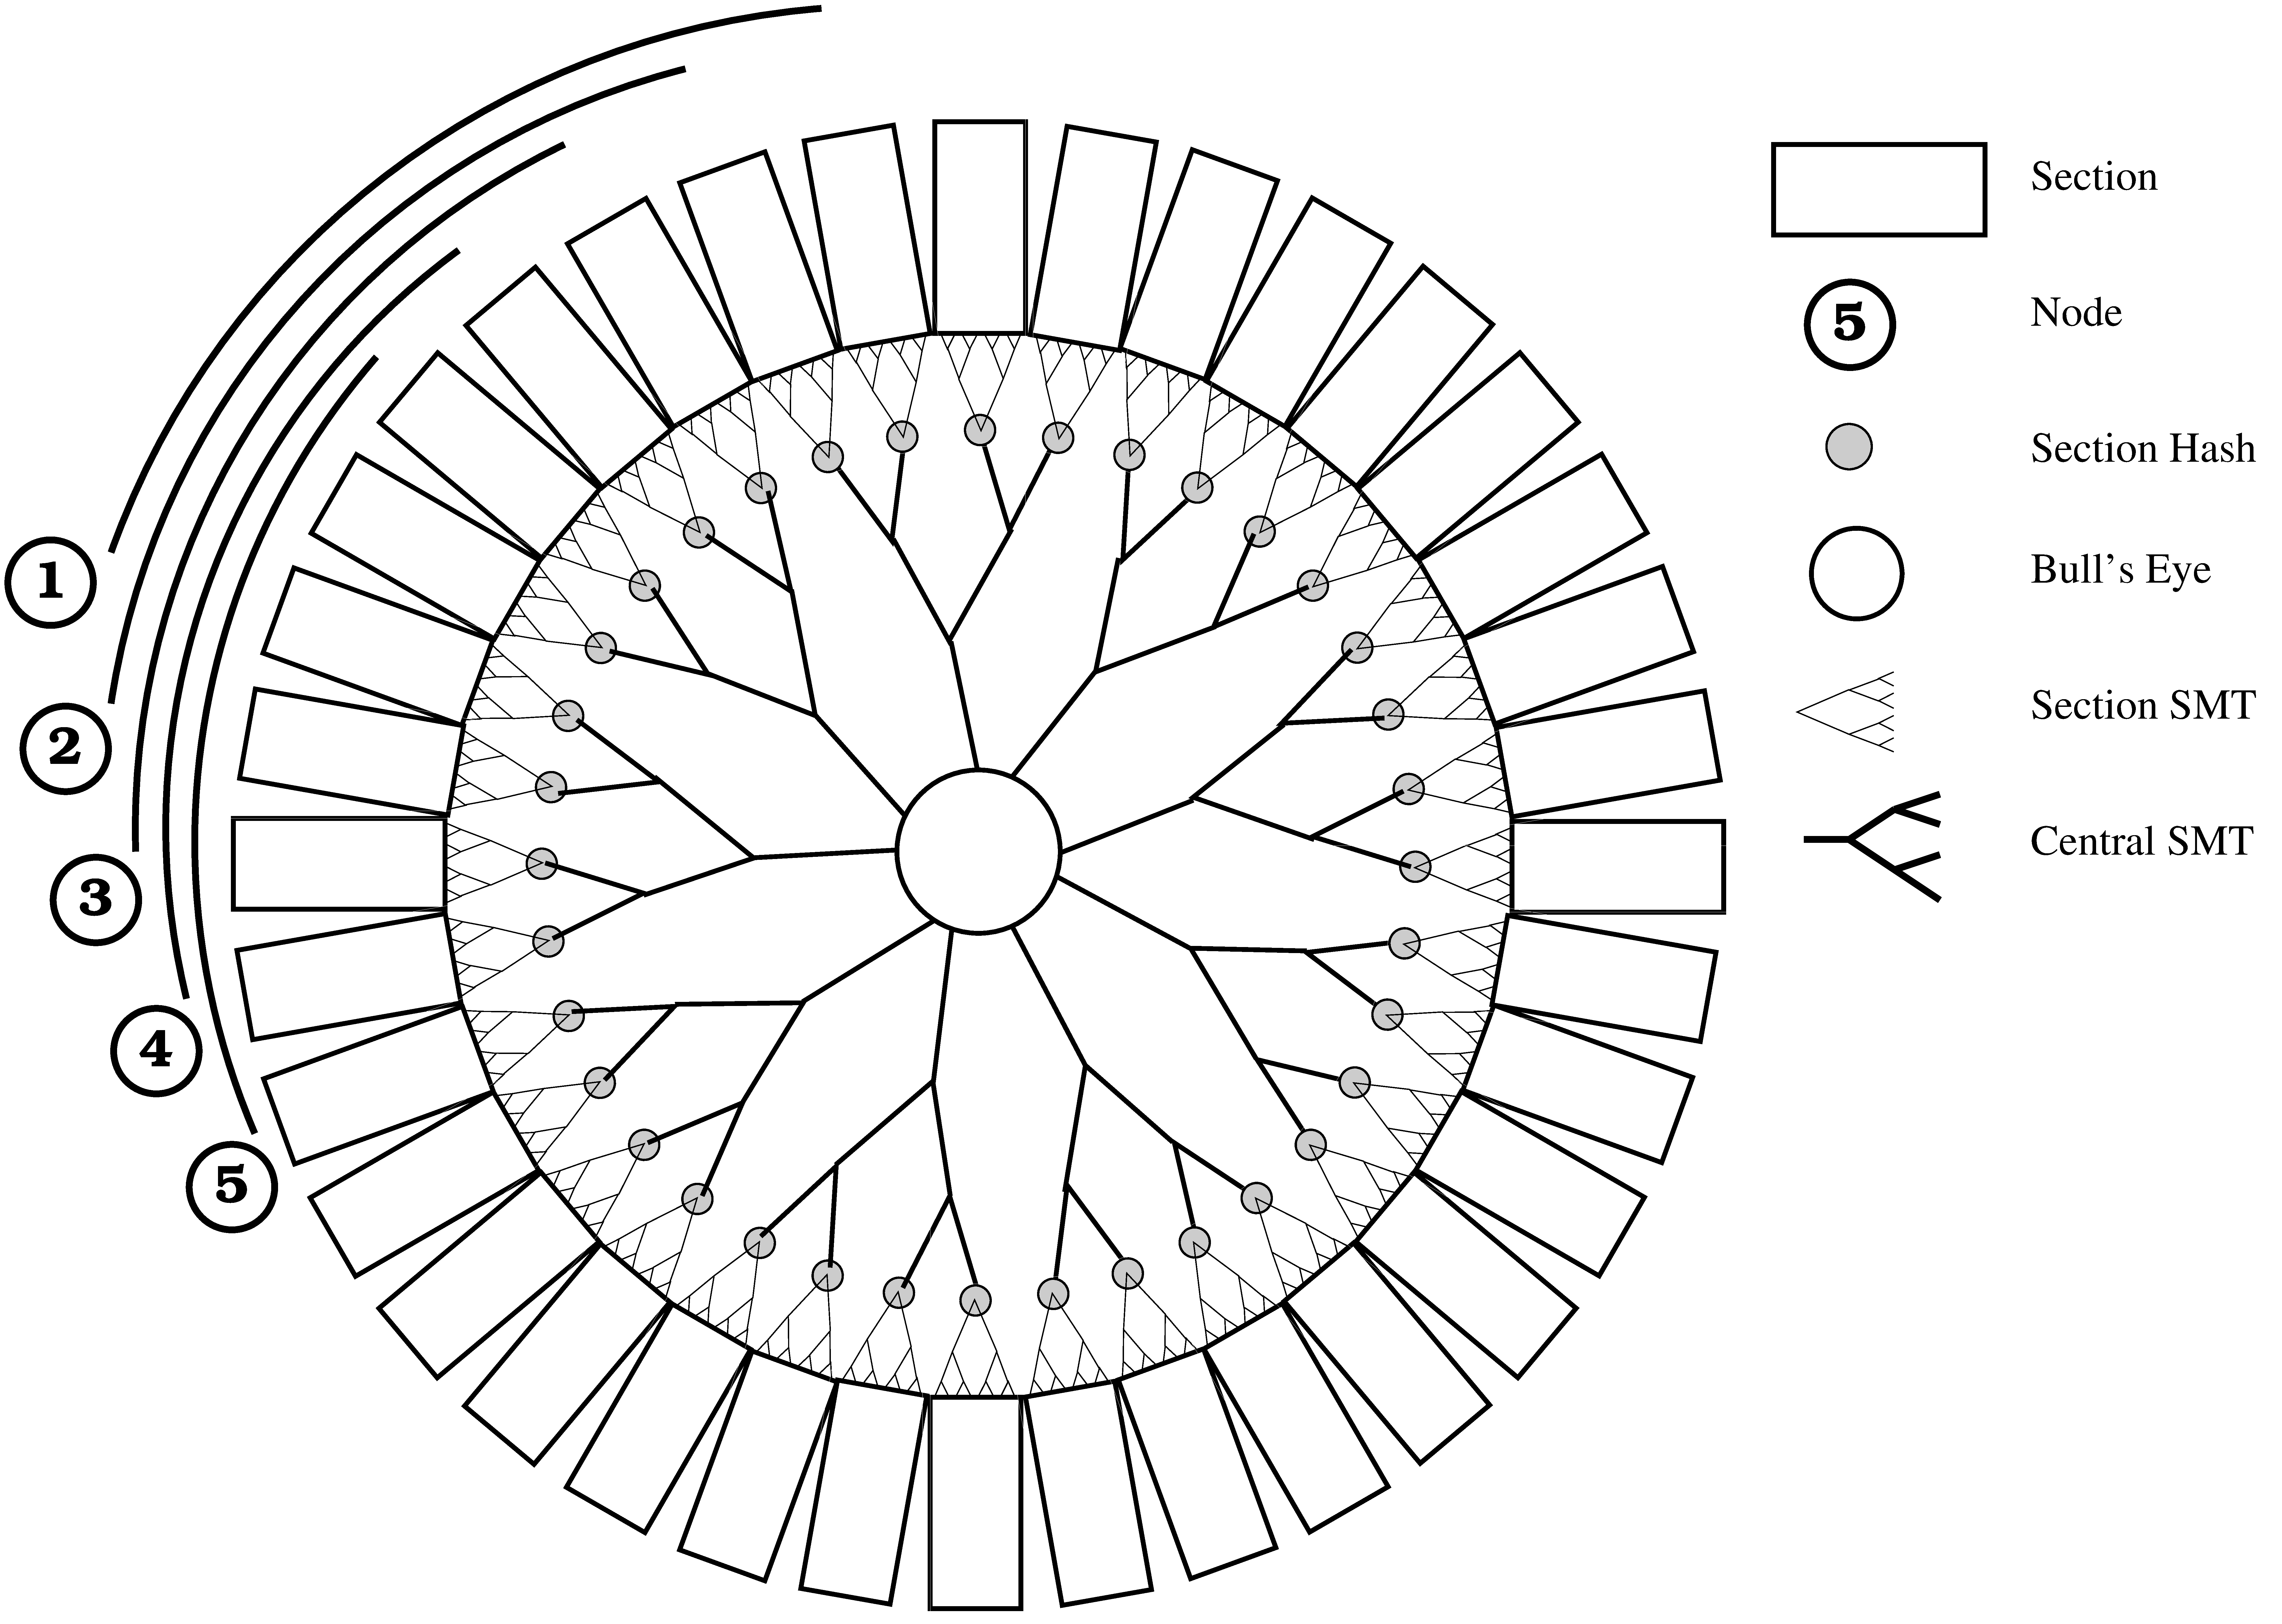
\includegraphics[width=1.0\textwidth]{fig/dart_bw.eps}
 % dart_bw.eps: 17766x12625 px, 300dpi, 150.42x106.89 cm, bb=0 0 4264 3030
 \caption{The structure of the DART database}
 \label{fig:dart}
\end{figure}


The hash-table is distributed between the nodes in the network, where each node manages a sample of sections. A section must be managed by more than Q nodes to keep redundancy and security of the data.
Each node must maintain the database sections within the node's section angle. This means adding and removing the transaction and updating the Merkle-tree root of the section hash.
The DART is updated according to the transaction list in an epoch generated by the network. The scripting engine will evaluate actions in the epoch and decide if an archive should be added, removed or selected. The selection of an archive means that the archive is sent back to the network and deleted from the DART. When a node updates a section, it must calculate the Section Merkle-root and sign it and send it to the network.
The signed section and the selected archive are distributed to the network via the gossip protocol. Each node will collect all the signed roots of the updated section when the majority has been reached for all updated sections. The node must calculate the Bull's eye (Merkle root) of the DART and sign and distribute the information via the gossip protocol. When the majority of the nodes in the network has reached a consensus of the Bull's eye value, the DART is considered to be updated.
If no consensus has been reached for DART, the current transaction in the epoch must be dropped, and the DART must revert to the previous state.
The Bull's eye value is stored in a hash-linked chain of blocks where each block points to the previous block's hash. Each block contains the Bull's eye pointer and a block number. It ensures data integrity, the state of the database. The concept is shown in the figure below.

\begin{figure}[H]
 \centering
 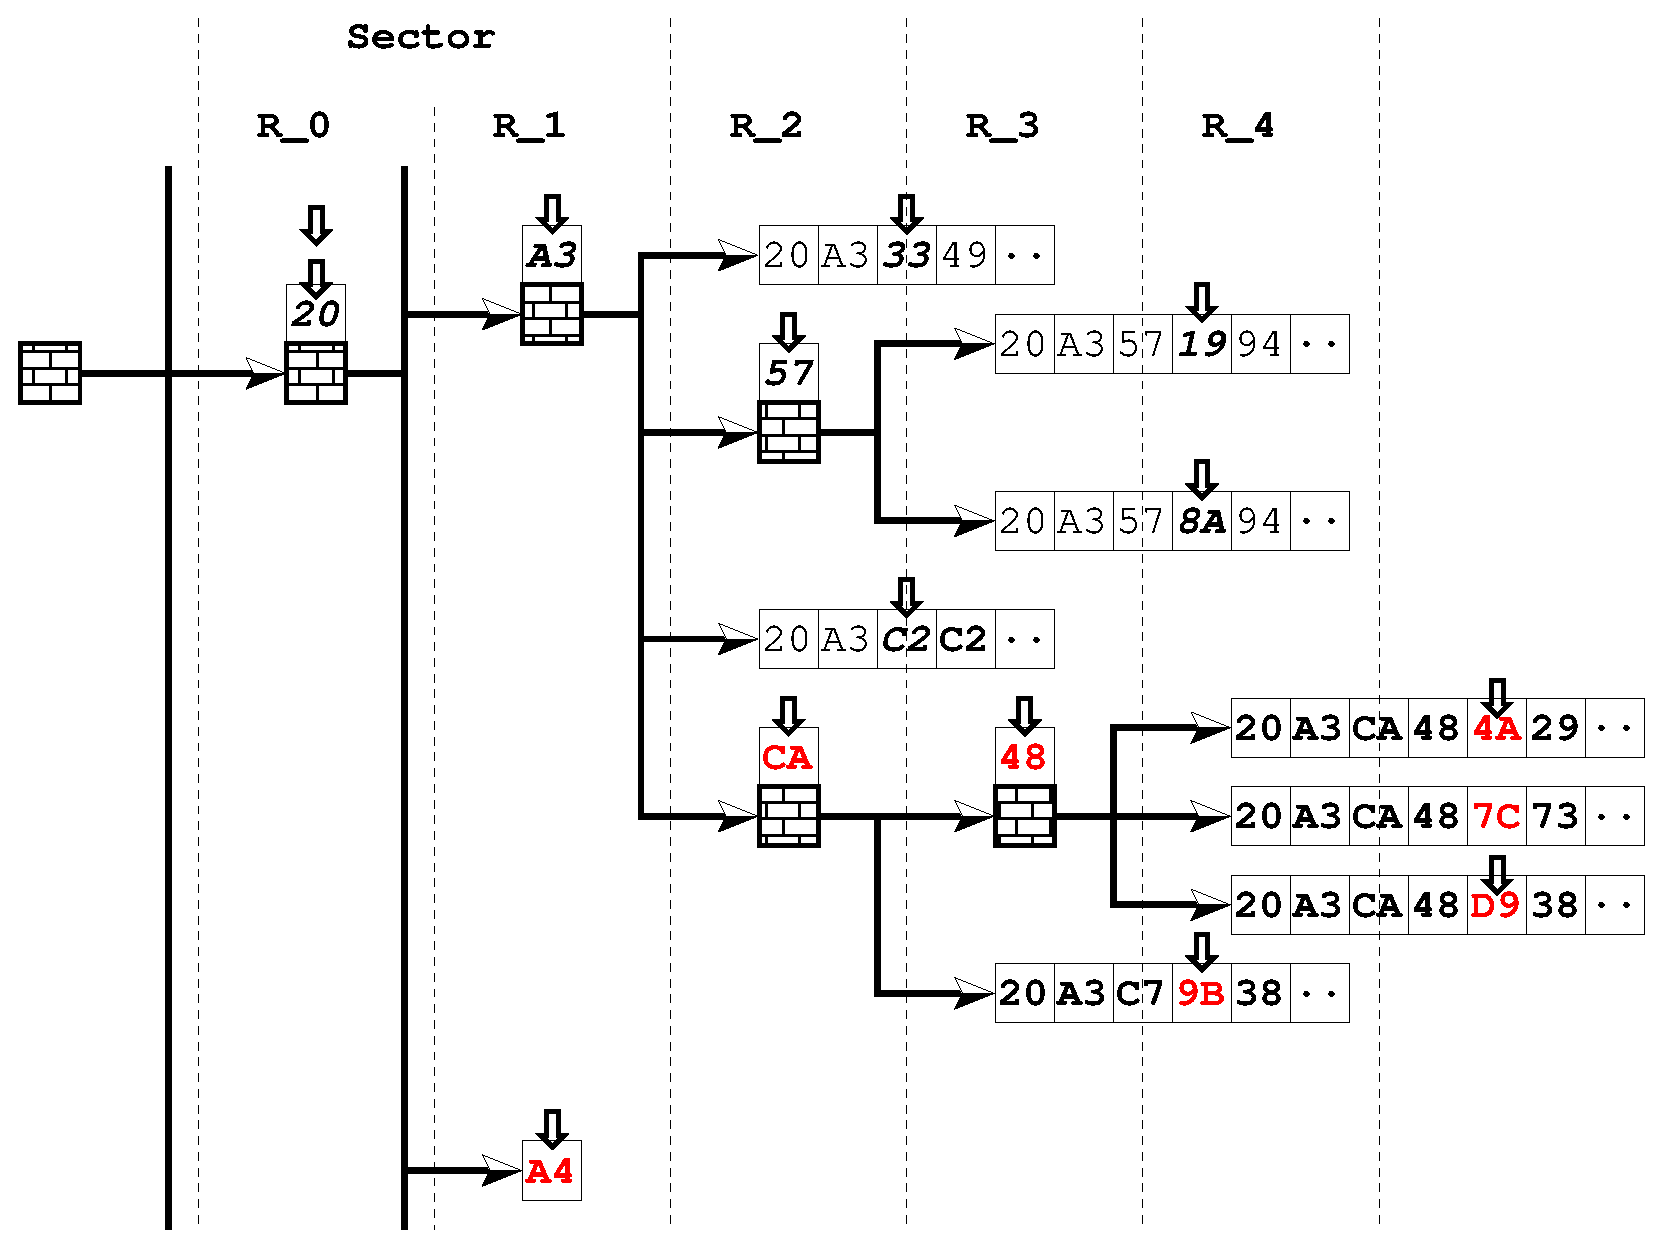
\includegraphics[width=1.0\textwidth]{fig/dart_tree_bw.eps}
 % dart_bw.eps: 17766x12625 px, 300dpi, 150.42x106.89 cm, bb=0 0 4264 3030
 \caption{The data structural layout of DART database}
 \label{fig:dart}
\end{figure}



\subsection{Sparse Merkle Tree}\label{sec:SMT}
The data in a section is mapped using a \abbrev{SMT}{Sparse Merkle Tree} which makes it efficient to add into and remove archives from the Merkle tree. \\
The hash point into the DART is divided by rims. Rim zero is the most significant byte (MSB) of the hash fingerprint of the archive. Rim one is the next byte in the hash etc. \\
In the current implementation of the DART, the first two rims are used as the section index. Thus the DART has a total number of indices $2^{16} = 65536$ which is equivalent to the two bytes unsigned number. \\
Each section stores the archive in a hash table. An SMT is used as a look-up table, and each rim is sectioned into a sub sparse Merkle tree. This means that rim two is the first SMT and rim three is the second SMT etc. \\ 
As a comparison, a traditional Merkle tree with $2^{24} = 8^3 \approx 16 \cdot 10^{6}$ Archives. Calculating a full Merkle tree requires the calculation of around $32 \cdot 10^6$ hashes. By contrast, using an SMT with $16 \cdot 10^{6}$  archives mean just around 2000 hashes have to be calculated.

\paragraph{Core protocol updates\\} 
The DART will be used for protocol updates by the following consensus. One or more nodes will need to run the new protocol update in a parallel DART containing the same transaction information as the current accepted DART. The new DART will have a new Bull's eye \abbrev{Bullseye}{DART Merkle Root}, and this will result in a fork of the Bull's eye chain. When the majority of the nodes run the newly upgraded nodes, they can decide to drop support for the old DART and run the new DART. When enough nodes stop running the old DART, it will not be able to reach a consensus, and the upgrade has completed.

\paragraph{DART garbage collection\\} 
A garbage collection script will run every (G) epoch and remove all the bills which are older than a specified date. Bills that have not been used for a long period will be burned, which ensures that the system does not contain dead bills/money.
It is the owner's responsibility to recycle their bills before the expiry date.


\paragraph{Unpredictable Deterministic Random\\}
The merkle root \bfit{Bullseye} is used as seed for the \abbrev{UDR}{Unpredictable Deterministic Random}, which is used in the different algorithmic consensus for the network.
 

\pagebreak
\section{Special Records}

The archives are stored in the DART using the hash-fingerprint as an index-pointer like in \abbrev{DHT}{Distribute Hash Tabel} (See \cref{sec:DART}). The hash of an archive is calculated in two ways as follows. If the archive does not contain $\#'param'$ the hash is calculated from the binary data of the HiBON archive and if the $\#'param'$ exists this type of archive is call \abbrev{PIA}{Parameter Indexed Archive}. For a PIA the hash-pointer is calculated for the content of the $\#'param'$.

The parameter starting with a dollar sign is reserved for use as system parameters (like $\$'param'$) and should only be used for as such, or else the system will reject it as an error.
In particular, $\$type$ is used to set the type of an HiBON object.
An PIA-archive must contain a $\$type$ parameter.

Some of the parameters in this special archive has restricted access.
The access \texttt{ro} means that this parameter is set on the creation of the archive and can not be changed. The \texttt{rc} access means that this parameter is controlled and updated by the network and can only be read. 


\subsection{Name card contract} \label{sec:name_card_contract}
A \abbrev{NNC}{Network Name Card} is a record which are composed of two archives \abbrev{NCL}{Name Card Label} and \abbrev{NCR}{Name Card Record} both of the archives are stored in the DART.

The NCL label card sets the NNC name and NCR record stores the data related to the name-card (see \cref{tab:ncr}). The two archives are always updated in pairs in the network.

The hash-pointer of an NCL is calculated for the name-parameter and not for the archives in itself. The NCL can and must only contain the parameter as shown in the  \cref{tab:ncl}.

When an NNC is updated the NCR is updated, the $\$previous$ hash-pointer is set to the previous NCR and the $\$index$ is increased by one. The $\$record$ parameter in NCL is set to the hash-pointer of NCR and $\$sign$ is set to the signature of $\$record$.

The $\$index$ of the first NCR is set to $0$, and the $\$previous$ parameter is to hash value of $\$pubkey$ of the NCL archive.

The $\$lang$ sets the type of restricted letters and symbols which is allowed to be used in the NNC name.


\begin{table}[H]
\begin{center}
\begin{tabular}{|l|p{7cm}|p{1.5cm}|l|}
      \hline
      Parameter & Description & Type & Access \\
      \hline
      $\$type$ & Set contract type to 'NCL' & \texttt{string} & \texttt{ro} \\
      \hline
      $\#name$ & Name of the name-card & \texttt{string} & \texttt{ro} \\
      \hline
      $\$lang$ & Language letter code & \texttt{string} & \texttt{ro} \\
      \hline
      $\$time$ & Creation date & \texttt{utc} & \texttt{ro} \\
      \hline
      $\$pkey$ & Public key & \texttt{ubyte[]} & \texttt{ro} \\
      \hline
      $\$sign$ & Signature of the $\$record$ & \texttt{ubyte[]} & \texttt{rc} \\
      \hline
      $\$record$ & Hash pointer to the NCR archive & \texttt{ubyte[]} & \texttt{rc} \\
      \hline
  \end{tabular}
\end{center}
\caption{NCL Network Name Card} 
\label{tab:ncl}
\end{table}

\begin{table}[H]
\begin{center}
\begin{tabular}{|l|p{7cm}|p{1.5cm}|l|}
      \hline
      Parameter & Description & Type & Access \\
      \hline
      $\$type$ & Sets the contract type to 'NCR' &  \texttt{string} & \texttt{ro} \\
      \hline
      $\$name$ & Hash value of the $NCR.\$name$ & \texttt{ubyte[]} & \texttt{ro} \\
      \hline
      $\$previous$ & Hash pointer to the previous NCR & \texttt{ubyte[]} & \texttt{rc} \\
      \hline
      $\$index$ & Index number & \texttt{uint} & \texttt{rc} \\
      \hline
      $\$node$ & Optional node record & \texttt{\#} & \texttt{rc} \\
      \hline
      ... & ... &  ... &  ... \\
      \hline
  \end{tabular}
\end{center}
\caption{NCR Network Name Record} 
\label{tab:ncr}
\end{table}




\subsection{Node contract}

\abbrev{NNR}{Network Node Record} is used to store the node data of the record

\begin{table}[H]
\begin{center}
\begin{tabular}{|l|p{7cm}|p{1.5cm}|l|}
      \hline
      Parameter & Description & Type & Access \\
      \hline
      $\$@$ & Set contract type to 'NNR' &  \texttt{string} & \texttt{ro} \\
      \hline
      $\#node$ & Public key for the node &  \texttt{ubyte[]} & \texttt{ro} \\
      \hline
      $\$name$ & Hash value of the $NCR.\$name$ &  \texttt{\#} & \texttt{ro} \\
      \hline
      $\$time$ & Creation date &  \texttt{utc} & \texttt{ro} \\
      \hline
      $\$sign$ & Signature of $\$name$ by $NCR.\$pkey$ &  \texttt{ubyte[]} & \texttt{rc} \\
      \hline
      $\$state$ & The state of the (\bfit{PN}, \bfit{N}, \bfit{AN})  &  \texttt{uint} & \texttt{rc} \\
      \hline
      $\$gene$ & Node gene bit-string&  \texttt{ubyte[]} & \texttt{rc} \\
      \hline
  \end{tabular}
\end{center}
\caption{NNR Network Node Record} 
\label{tab:node_record}
\end{table}

\subsection{Hash Lock Record}
This record is used to store the has of an full-hash-value of the record with a $\#'param'$ to secure that the Merkle root of the DART.

\begin{table}[H]
	\begin{center}
		\begin{tabular}{|l|p{7cm}|p{1.5cm}|l|}
			\hline
			Parameter & Description & Type & Access \\
			\hline
			$\$@$ & Sets the contract type to 'HL' &  \texttt{string} & \texttt{ro} \\
			\hline
			$\$lock$ & Raw hash value of full $\#$ record  & \texttt{ubyte[]} & \texttt{ro} \\
			\hline
		\end{tabular}
	\end{center}
	\caption{HL Hash Lock} 
	\label{tab:hl}
\end{table}


\subsection{Sub-Network contract}

Via a special contract executed on the \abbrev{TMN}{Tagion Main Network} a \abbrev{TSN}{Tagion Sub Network} can be launched. This sub-network will create a new sub-DART which only can be updated from the nodes running the TSN.\\
A group of nodes can initiate the sub-network by signing this contract and stake an amount in TGS.\\
The rules for the TSN are set when the network is launched, and the rules can differ from the rules in TMN.
The TSN can be assigned to a group of nodes or fully open for all nodes. When a TSN is launched an \abbrev{TSNF}{Tagion Sub Network Funds} is created on the main network to hold the funds for the fees in the main network. The funds are used to pay rewards to the nodes running the TSN and to pay fees to the main.
When an epoch is created in the bull's eye for TSN, a contract is automatically sent to the MTN, and a fee is deducted from the TSNF account and burned.
If there are not enough funds in the TSNF account, TMN rejects the contract.

TGS used in the TSN must be locked in a \abbrev{TSNA}{Tagion Sub Network Account} these funds can only be transferred between other TSNA and to the TSNF. Funds can not be transferred from TSNF to a TSNA.

The funds in TSNA can be transferred to TGS-bills again via TSNA-contract this contract can take multiple TSNA as input and will transfer all the funds to bills on the output, all the input TSNA will be deleted from DART as is the case with TGS-bills.

\paragraph{Basic rules for a Sub-Network}
\begin{enumerate}[\S 1]
 %\item TGS is accounted in TMN
 \item TSN can have a different rule set then applies for TMN
 \item No nodes can transfer money out of a TSNF account
 \item An TSNF account is used to pay rewards to the TSN nodes and the burning fees to the TMN
 \item An TSNA account funds can be transferred to a TSNF account
 \item An TSNA account can transfer money to other TSNA accounts. The fees burned are a little higher than fees for bills.
 \item The rewards in the TSN are paid from the TSNF account because a TSN can not print TGS as rewards as is the case for TSN.
\end{enumerate}



\pagebreak
\input{tvm_engine}

\pagebreak
\section{Transaction Scripts}
When the network receives a transaction request, it is added in an epoch and executed by the scripting engine. A transaction request includes a transaction object which is a data package in HiBON format. The HiBON object contains input bill numbers and the transaction script including a list of digital signatures which signs the transaction script object. The signatures can be verified via the public keys represented in the input bills.

\begin{table}[H]
\begin{center}
\begin{tabular}{|l|p{7cm}|p{1.5cm}|l|}
%
\hline
Parameter & Description & Type & Access \\
\hline
$\$type$ & Set contract type to 'B0' &  \texttt{string} & \texttt{ro} \\
\hline
$\$V$ & Value & \texttt{ulong} & \texttt{ro} \\
\hline
$\$k$ & Epoch number & \texttt{uint} & \texttt{ro} \\
\hline
$\$T$ & Bill type & \texttt{string} & \texttt{ro} \\
\hline
$\$Y$ & Doubled hashed Owner key & \texttt{ubyte[]} & \texttt{ro} \\
\hline
{...} & {...} & {...}  & {...} \\
\hline
\end{tabular}
\end{center}
\caption{Standard archived Bill object}
\label{tab:standard_bill}
\end{table}

\begin{table}[H]
\begin{center}
\begin{tabular}{|l|p{7cm}|p{1.5cm}|l|}
%
\hline
Parameter & Description & Type & Access \\
\hline
$\$in$ & Array of Bill numbers and public keys & \texttt{[]} & \texttt{ro} \\
\hline
$\$read$ & Array of Bill numbers and public keys & \texttt{[]} & \texttt{ro} \\
\hline
$\$out$ & Array of public key hashes & \texttt{[]} & \texttt{ro} \\
\hline
$\$params$ & Parameters used by the script & \texttt{\{\}} & \texttt{ro} \\
\hline
$\$script$ & Transaction script & \texttt{\{\}} & \texttt{ro} \\
\hline
\end{tabular}
\end{center}
\caption{Transaction scripting object}
\label{tab:transaction_scripting_object}
\end{table}

\begin{table}[H]
\begin{center}
\begin{tabular}{|l|p{7cm}|p{1.5cm}|l|}
%
\hline
Parameter & Description & Type & Access \\
\hline
$\$record$ & Scripting object & \texttt{\{\}} & \texttt{ro} \\
\hline
$\$signs$ & Array of input signatures & \texttt{[]} & \texttt{ro} \\
\hline
\end{tabular}
\end{center}
\caption{Transaction object}
\label{tab:transaction_object}
\end{table}

\paragraph{Transaction Epoch consensus rules:}
\begin{enumerate}
 \item 
 If one or more script objects is found with the same input bill number, the first transaction object in the epoch is kept in the epoch list. Any other object flows in the list are removed.
\end{enumerate}


\paragraph{Transaction object initial consensus rules:}
\begin{enumerate}
 \item 
    The size of the inputs array in the script record must be one or more.
 \item 
    The size of the inputs array and the signature arrays must be the same size.
 \item 
    The bill type of the first type input must be a Tagion type.
 \item 
    Duplicate bill numbers are not allowed.
 \item 
    All the inputs must be in the current state of the DART.
\end{enumerate}
If a transaction object violates one of the initial consensus rules, it is handled by a violation script function.

\paragraph{Transaction scripting execution:}
Because the epoch list is guaranteed to prevent inputs with same bill number, a node can choose to execute the scripts in the epoch in parallel.

\paragraph{First execution procedure and rules:}
\begin{enumerate}
 \item 
    The bills within the node's DART angle are read from the DART. 
 \item 
    The read bills are gossiped to the network.
 \item 
    If the script object has only one input, the script is immediately executed.
 \item 
    If all the bills in the inputs are covered in the local DART, the script is executed immediately.
\end{enumerate}

\paragraph{Second execution procedure and rules:}
\begin{enumerate}
\item 
    The script is executed if all the inputs are received or read for a transaction object and the signatures are correct.
\item
    The script must finish with a burn function which burns the transaction fee.
\item 
    If the sum of all outputs of the bill type Tagions (bill type can be Tagions or external contracts of, e.g. Euros) is greater than the sum of the input minus the transaction fee, the first input bill is scheduled to be removed, and the transaction is ignored.
\item 
    If the sum of all outputs of types other than Tagion is greater than the input, the first input bill is scheduled to be removed, and the transaction is ignored.
\end{enumerate}

\paragraph{DART execution procedure:}
\begin{enumerate}
 \item 
    When all scripts have been executed, the process of updating the DART begins.
 \item 
    All inputs of successfully executed scripts must be removed from sections covered by the node.
 \item 
    All outputs of the successfully executed script must be added to the sections covered by the node.
 \item 
    All the Merkle roots within the section angle must be calculated and signed and gossiped to the network.
Note: From this point, the node can start executing the next epoch.
 \item 
    When the node has received the majority for all the sections' Merkle, it calculates the Bull's eye of the DART, which is signed and gossiped to the network.
 \item 
    When the majority of consistent Bull's eyes has been received, the node decides that the DART has been updated and changes states. 
Note: A transaction has been completed at the new state.
 \item 
    If one of the above rules fails, the DART is reverted to the previous state.
\end{enumerate}

Note: When a node receives a transaction object, it can send a request to the DART to collect the inputs of the script. By doing the execution in parallel, it improves the transaction time instead of starting to collect inputs when the epoch has been completed.



\pagebreak
\section{Business Model}
The business model consists of two parts, namely incentives and fee payments. The incentives are given to the nodes for their work and fees are paid by the users for using the system. 

\paragraph{Money printing - incentives }
New money is added to the system when an epoch has been completed, and the DART has reached a consensus. The newly printed money is rewarded to one of the active nodes if it has successfully executed the epoch. \\
The reward winning node is selected via a UDR Lottery, which is seeded from the bull’s eye hash of the DART where the epoch was generated. \\
The amount is calculated by an economic protocol controlled by the economic governance, see \cref{subsec:economic_governance}. \\

\paragraph{Money burning - payment}
When a transaction is performed in the network, more fees are paid by the user initiating the transaction. The fees depend on storage, the transaction amount and the script execution load. The fees paid to the network are burned; thus, the amount is taken out of the money supply.
A storage fee is paid per bytes of the total sum of bytes of all outputs stored in the DART. \\
A transaction fee is paid as a fraction of the total Tagion amount of the input of the transaction script. \\
The execution fee is calculated per script instructions where each instruction is priced. \\
If the total Tagion amount of the output transaction script is less than a specified limit, the whole amount is burned and the transaction is not valid.
Fees for decentralised exchanges are described in \cref{sec:dex}.


% The broker contarct is removed for now
%\pagebreak
%\section{Economic Contracts}
The Tagion network is designed to handle multiple currencies by using the Tagion as the exchange currency.
The other currencies in the network are represented by a bill type and are fully backed by a broker who guarantees the currency.
Multi-Currency Smart Contract
A broker is set up with a Multi-Currency Smart Contract (MCSC), which contains information about the currency type, account ID, and the broker’s public key. The total value of the broker's account is accounted for in the global value record. The MCSC contract is a special type of bill which will not be garbage collected automatically. 

\begin{table}[H]
\begin{center}
\begin{tabular}{|p{2cm}|p{7cm}|p{2cm}|}
\hline
Parameter & Description & Type \\
\hline
broker & Identity information object & mandatory \\
\hline
T & Currency type & mandatory \\
\hline
accointid & Account ID which labels a parameter in the global value record & mandatory \\
\hline
y & Public key & mandatory \\
\hline
\end{tabular}
\end{center}
\caption{Broker multi-currency smart contract (MCSC)}
\label{tab:MCSC}
\end{table}

\begin{table}[H]
\begin{center}
\begin{tabular}{|p{2cm}|p{7cm}|p{2cm}|}
\hline
Parameter & Description & Type \\
\hline
B & Bill pointer to the (MCSC) & mandatory \\
\hline
G & Guaranteed value & mandatory \\
\hline
V & Value in circulation & mandatory \\
\hline
\end{tabular}
\end{center}
\caption{Broker value record which is stored in the global value record}
\label{tab:broker_value_record}
\end{table}

\paragraph{Exchange contract\\}
All the currencies which are represented on the network can be exchanged to Tagion via an Exchange Smart Contract (XSC). \\
To execute an XSC, a normal transaction is performed with some additional parameters. The only significant difference from a transaction contract is that an XSC is a type of contract executed in the exchange matching pool. That means that asks and bids are matched according to the epoch ordered list. \\
If an XSC is not yet executed, the contract can be called back. If called back, the contract is erased from the exchange matching pool via an EXSC contract (Erase exchange Smart Contract) – or the contract can self-destroy by setting a lifetime for the contract. \\
\paragraph{Off-ramp contract\\}
An off-ramp contract, OXSC (Off-ramp eXchange Smart Contract), is performed when the owner of a bill asks their broker to pay out to an external account. \\
All the OXSC’s are collected in an off-ramp exchange pool. The broker needs to sign the output from this contract, and the off-ramp bill is burned.


\pagebreak
\section{Parallelism}
Transactions with independent bills can run in parallel, enabling scalability and performance. Independent bills mean that inputs and outputs of transactions are not the same bills. It can run in parallel because the overall design of the data, DART and the scripting engine makes it possible. \\
The scripting engine is an event-driven engine that executes functions in parallel with inputs and produces outputs locally on each node. Inputs which must be used are read from the DART, and the outputs are stored in the DART. When the transaction successfully completes, the inputs are deleted.

The database is distributed, thus nodes only maintain and keep a copy of the part of the database they are subscribed to, see \cref{sec:DART}. Because transactions' inputs and outputs are independent and each node only executes a part of the transactions, they can be executed in parallel and the database updated in parallel as well. \\
It is not the transaction instructions, which are stored in the database, but the actual bills, which are used as inputs and outputs. Then all nodes do not need to execute all data to verify the integrity of the database as in typical blockchain structures. The consensus event and consensus data are thus merely an intermediate calculation, where the output is stored. 


%\pagebreak
%\input{node_stack}

\pagebreak
\section{Privacy}
The current banking system achieves a level of privacy by keeping key information hidden from the public. Under this regime, all identities are known by the trusted third party, i.e. the bank.

In the Tagion system, all transactions and bills are public, but physical identities are separated from transactions and bills. The system has full transparency regarding how many bills exist. A public key is bound to a bill and not an account, and the private key is for signing and spending the bill.\\

\begin{figure}[H]
 \centering
 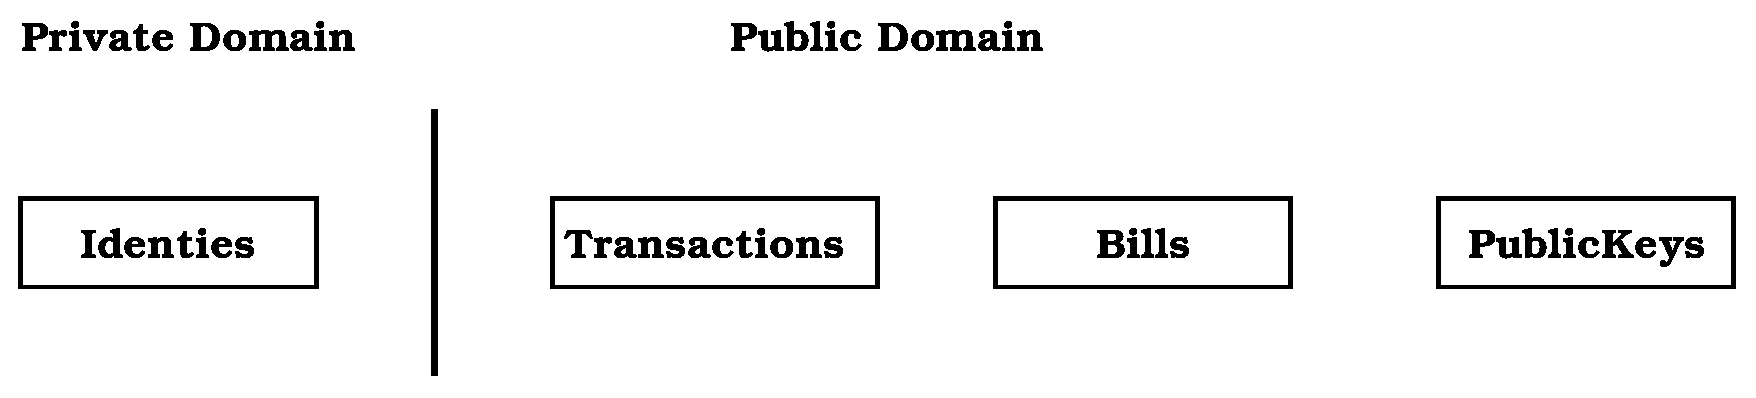
\includegraphics[width=0.8\textwidth]{fig/privacy.eps}
 \caption{Private and Public domain}
 \label{fig:private_domain}
\end{figure}

Tagion bills are not linked in a chain because each time a bill is spent, a transaction is recorded in the database, deleting the old bill and creating a new one. A full trace of the network will, however, reveal the inputs and outputs of transactions, thus linking the bills. Over time, the bills split and re-combine as they become part of multiple in and out transactions. Therefore, it is not feasible to search back through the linking of bills for a pattern, because it is not a 1:1 trace of bills and would cause an NP (non-polynomial) problem, which cannot be solved in finite time.\\

\begin{figure}[H]
 \centering
 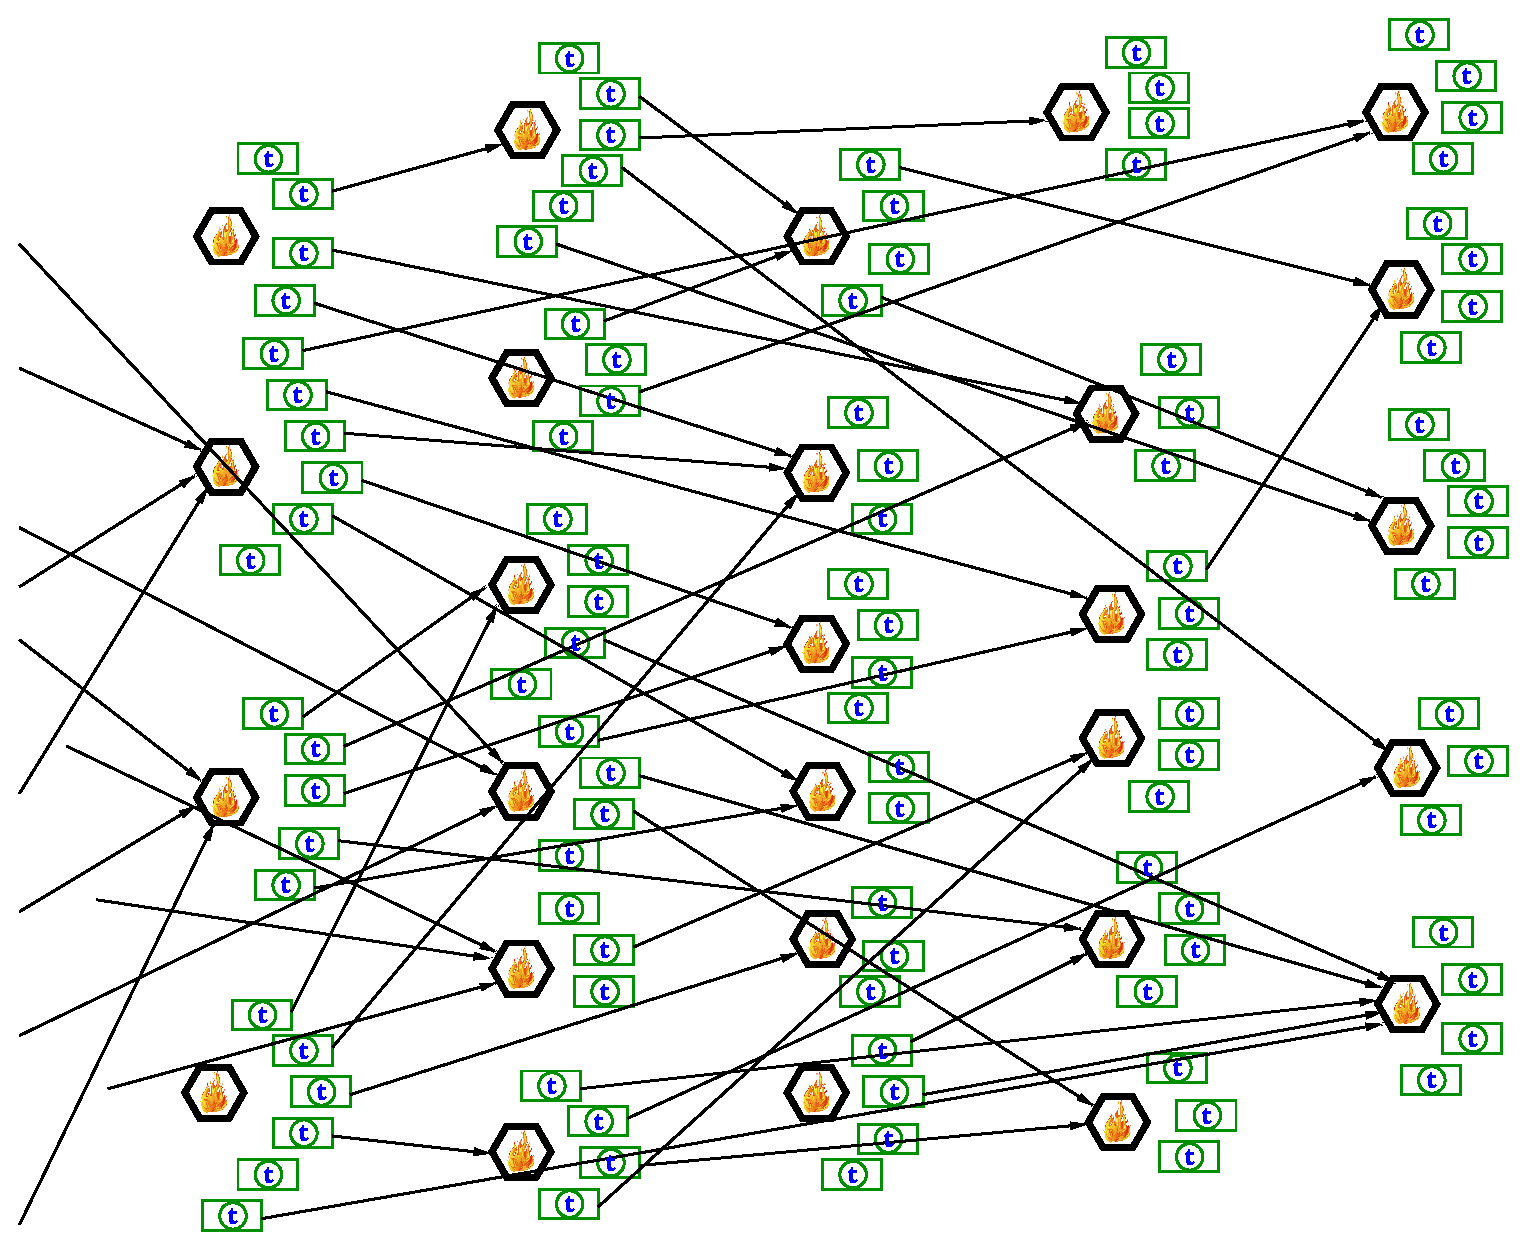
\includegraphics[width=0.9\textwidth]{fig/transaction_inout.eps}
 \caption{A transaction is represent as a hexagon with a flame the small-bank-note with a {\bfseries{t}} represent bills}
 \label{fig:transaction_inout}
\end{figure}

A user can determine if the same public key should be the owner of all his/her bills or a different, derived, public key. They can hold a different public key for each owned bill, and these keys may not correlate with each other. By using a different public key for each node, a user can make transactions in full privacy, i.e. anonymously.\\ 
A node is a public servant and therefore needs to reveal public information. A node in the Tagion system needs to use a fixed public key to ensure the governance of the node. The public key is the identifier for the node that can be perceived as an account, and it is the account for receiving rewards.\\ 


%\pagebreak

%\input{sub_network}

\pagebreak
\section{Decentralised Exchange using Lightning Network} \label{sec:dex}

Via a TSN, interfacing other alien \abbrev{DLT}{Distributed Ledger Technology} for exchanges is possible. Most of the current DLTs are based on \abbrev{POW}{Prof Of Work} which secures the immutability of the ledger and has been proven to be very robust. The downside for those types of DLT is the long confirmation time.\\
A suggested solution to decreasing the confirmation time is to use a second layer solution using a network of payment channels like the \abbrev{LN}{Lightning Network}.\\
\abbrev{TN}{Tagion Network} and LN support each other to enable a \abbrev{DEX}{Decentralised Exchange} for DLT networks which support full-duplex payment channels, \abbrev{HTLC}{Hashed Time Lock Contract} and \abbrev{MultSig}{Multi Signature}.
The advantage of using the TN as a support system to store intermediate data for the payment channels is that the LN-nodes can share data even if some of the LN nodes go offline.
In the current LN use in Bitcoin and other similar networks, the routing between the payment channels is a challenge. One of the reasons for this is that the routing tables are difficult to share and maintain between the nodes. In Tagion, because data is stored in a DART this makes sharing data feasible.\\
Because funds in an alien DLT can be locked via an HTLC, the \abbrev{ALC}{alien-currency} the funds can be swapped with the native tagion-currency in an atomic manner. This feature enables the Tagion network to support exchange functionality in a decentralised manner providing full liquidity because all exchange pairs have Tagions as the counterpart.\\

\subsection{Trading flow using Lightning and Tagion Network}
The Tagion network can order the bids/asks in a \abbrev{BFT}{Byzantine Fault Tolerant} manner. This means that the network is able to come to a consensus on the order of transactions and this solves the matching and prices discovery in a fair manner and solves front-running the order-book in a decentralised manner.

The idea is one STN handles only one trading pair between TGS and ALC. By only using one pair, the matching and routing problem is reduced significantly in comparison to a full multi-currency-DEX with more than two currencies.\\
First of all, the price discovery is more straightforward, and the amount of data to process is much less if only one pair must be matched and discovered. The second advantage of the one pair DEX is that sub-networks only need to handle one alien smart contract format.\\

\subsubsection{Price discovery and matching}

The DEX are able to handle two types of orders as shown in \cref{tab:dex_acl_tgn} and \cref{tab:dex_tgn_acl}.
The orders are sent to the TN and at each epoch the trade-order-queue is sorted according to the hashgraph consensus ordering. 
\paragraph{Exchange order pairs}
\begin{itemize}
 \item[\bfit{ATO}] Order to buy TGS for ALC
 \item[\bfit{BTO}] Order to buy ALC for TGS
\end{itemize}

The matching-engine will maintain two sales-lists of \abbrev{ATO}{Ask Trade Orders} and a \abbrev{BTO}{Bid Trade Orders}, those sales-lists are sorted according to the exchange rate with the lowest exchange ratio at to top of the list. A detailed example can be found in \cref{sec:dex_example}.


The \bfit{ask} exchange rate is defined as:
\begin{equation}
 E_{ask} = \frac{Q}{P} ~\text{in unit} ~\left[ ACL/TGS \right]
\end{equation}

The \bfit{bid} exchange rate is defined as:
\begin{equation}
 E_{bid} = \frac{P}{Q}~\text{in unit} ~\left[ TGS/ACL \right]
\end{equation}

\begin{itemize}
 \item[$P$]is the price in TGS
 \item[$Q$]is the price in ACL
\end{itemize}


The trade-order-queue is maintained with the orders that are not executed. A new trade-order-queue is generated in each epoch and added in the end of the current trade-order-queue.
The matching executes the first in trade-order-queue, i.e. the oldest order is searched first for a match.

The ATO and BTO order in the trade-order-queue are defined as buyers.
A match is defined as found, when the buyer's exchange-rate is higher than or equal to the seller's exchange-rate from the corresponding sales-list. The price of the settlement will be set at the seller's exchange-rate.
\begin{itemize}
 \item 
When an ATO buys from BTO-sales-list at $E_{ask,BTO}$ price when:\\ $E_{ask,ATO} \geq E_{ask,BTO}$ or the same as $\frac{Q_{ATO}}{P_{ATO}} \geq \frac{Q_{BTO}}{P_{BTO}}$.
 \item 
When an BTO buys from ATO-sales-list at $E_{bid,ATO}$ price when:\\ $E_{bid,BTO} \geq E_{bid,ATO}$ or the same as $\frac{P_{BTO}}{Q_{BTO}} \geq \frac{P_{ATO}}{Q_{ATO}}$.
\end{itemize}

Summarising, a buyer with an ATO-order from the order-queue matches a seller with a BTO-order from the BTO-sales-list and vice versa. 
Then the size is calculated, and a trading-contract with the corresponding pair is generated and stored in the TN.

If the ATO or the BTO has sold the whole size, then the order is removed from the lists.\\
If an order includes a valid time period of $t$ and if the epoch consensus time is greater than this valid time period $t$ then the order is removed and not executed.

\begin{table}[H]
\begin{center}
\begin{tabular}{|l|p{7cm}|p{1.5cm}|l|}
      \hline
      Parameter & Description &  Type & Access \\
      \hline
      $\$type$ & Set the contract type to 'ATO' &  \texttt{string} & \texttt{ro}\\
      \hline
      $P$ & Price unit TGS &  \texttt{ulong} & \texttt{ro}\\
      \hline
      $Q$ & Price unit ACL &  \texttt{ulong} & \texttt{ro} \\
      \hline
      $size$ & Size of ACL &  \texttt{ulong} & \texttt{ro}\\
      \hline
      $lock$ & Random Hash-lock key &  \texttt{bin} & \texttt{ro}\\
      \hline
      $time$ & Valid time period &  \texttt{utc} & \texttt{ro} \\
      \hline
  \end{tabular}
\end{center}
\caption{ATO HiBON to buy TGS for ALC} 
\label{tab:dex_tgn_acl}
\end{table}

\begin{table}[H]
\begin{center}
\begin{tabular}{|l|p{7cm}|p{1.5cm}|l|}
      \hline
      Parameter & Description & Unit & Access \\
      \hline
      $\$type$ & Sets the contract type to 'BTO' &  \texttt{string} & \texttt{ro}\\
      \hline
      $P$ & Price unit TGS &  \texttt{ulong}& \texttt{ro}\\
      \hline
      $Q$ & Price unit ACL &  \texttt{ulong}& \texttt{ro} \\
      \hline
      $size$ & Size og TGS & \texttt{ulong}& \texttt{ro} \\
      \hline
      $lock$ & Random Hash-lock key & \texttt{bin} & \texttt{ro} \\
      \hline
      $time$ & Valid time period & \texttt{utc} & \texttt{ro} \\
      \hline
  \end{tabular}
\end{center}
\caption{BTO HiBON to buy ALC for TGS} 
\label{tab:dex_acl_tgn}
\end{table}


\subsubsection{Exchange execution rules}
\begin{figure}[H]
 \centering
 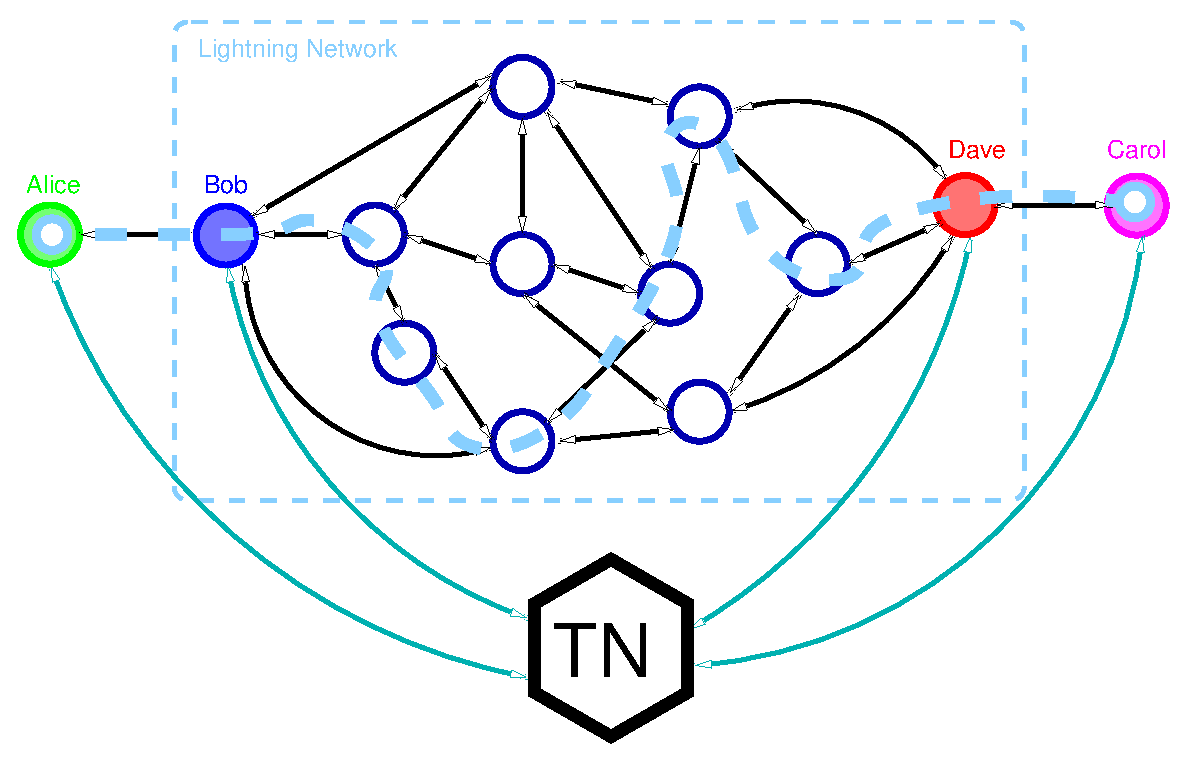
\includegraphics[width=1.0\textwidth]{fig/dex_ln.eps}
 % dart_bw.eps: 17766x12625 px, 300dpi, 150.42x106.89 cm, bb=0 0 4264 3030
 \caption{Tagion Decentralised Exchange based on Lightning Network  }
 \label{fig:dex_ln}
\end{figure}

In the following example, the execution flow of the DEX is described.


\paragraph{Alice wants to trade TGS for ALC (ATO). It can be done as follows.}

\begin{enumerate}[{A}.1]
 \item \textbf{Entry:} Alice opens an LN channel with Bob.
 \item Alice requests a trading channel from Bob with a guarantee of $\omega_{alice,S}$ in ALC 
 \item Bob locks up a guarantee of an amount $\tau_{bob,S}$ in TGS which matching Alice's $\omega_{alice,S}$ amount. Bob creates an HTLC lock it with $R_{bob}$ and send this information to the TN.
 \item Alice pays $\omega_{alice}$ to the contract lock with $R_{bob}$.
 \item \textbf{Order:} Alice sends an order to the TN including an HTLC contract to Bob locked with $R_{alice}$ and the amount $\alpha_{alice}$ in ALC. The information includes the bid/ask prices and HTLC contract which is sent to the TN.\\
 \textit{\textbf{Note:} Carol has previously locked funds with $R_{calor}$ in TGS to buy ALC}
 \item When the TN discoveries a trading pair matching Alice and Carol the network generated a TN-HTLC trading contract locked with both $R_{alice}$ and $R_{carol}$.
 \item When Bob verifies that, Carol has to reveal $R_{calor}$. Bob initials a route between Alice to Carol according to the trading bill. Bob also makes an HTLC return the rest of Alice's funds locked with $R_{alice}$.
 \item Alice reveals $R_{alice}$ and the funds can be transferred.
 \item \textbf{Exit:} Alice can ask Bob to reveal $R_{bob}$ and exit the trading channel. Bob's locked funds are returned, and Alice can claim her funds.  
\end{enumerate}

\paragraph{Carol wants to trade ALC for TGS (BTO). It can be done as follows}
\begin{enumerate}[{B}.1]
 \item \textbf{Entry:} Carol opens an LN channel with Dave.
 \item Carol requests a trade channel with Dave, both Carol and Dave guarantee $\tau_{carol,S}$ and $\tau_{dave,S}$ in TGS and hash-locked with $R_{carol}$ in the TN.
 \item \textbf{Order:} Carol sends an order to Dave via the TN.
 \item Dave receives a confirmation from the network about the order from Carol.  
 \item Dave and creates an HTLC contract to Carol locked with $R_{dave}$ at the amount of $\alpha_{carol,T}$ in ALC.
 \item When the TN discovers a trading pair matching Alice and Carol, the network generates a TN-HTLC trading contract locked with both $R_{alice}$ and $R_{carol}$.
 \item Dave reveals the $R_{dave}$ the Alice can execute the trade.
 \item \textbf{Exit:} Carol can ask Dave to reveal $R_{dave}$ and exit the trading channel. Dave's and Carol's locked funds are returned.  
 
\end{enumerate}

\begin{figure}[H]
 \centering
 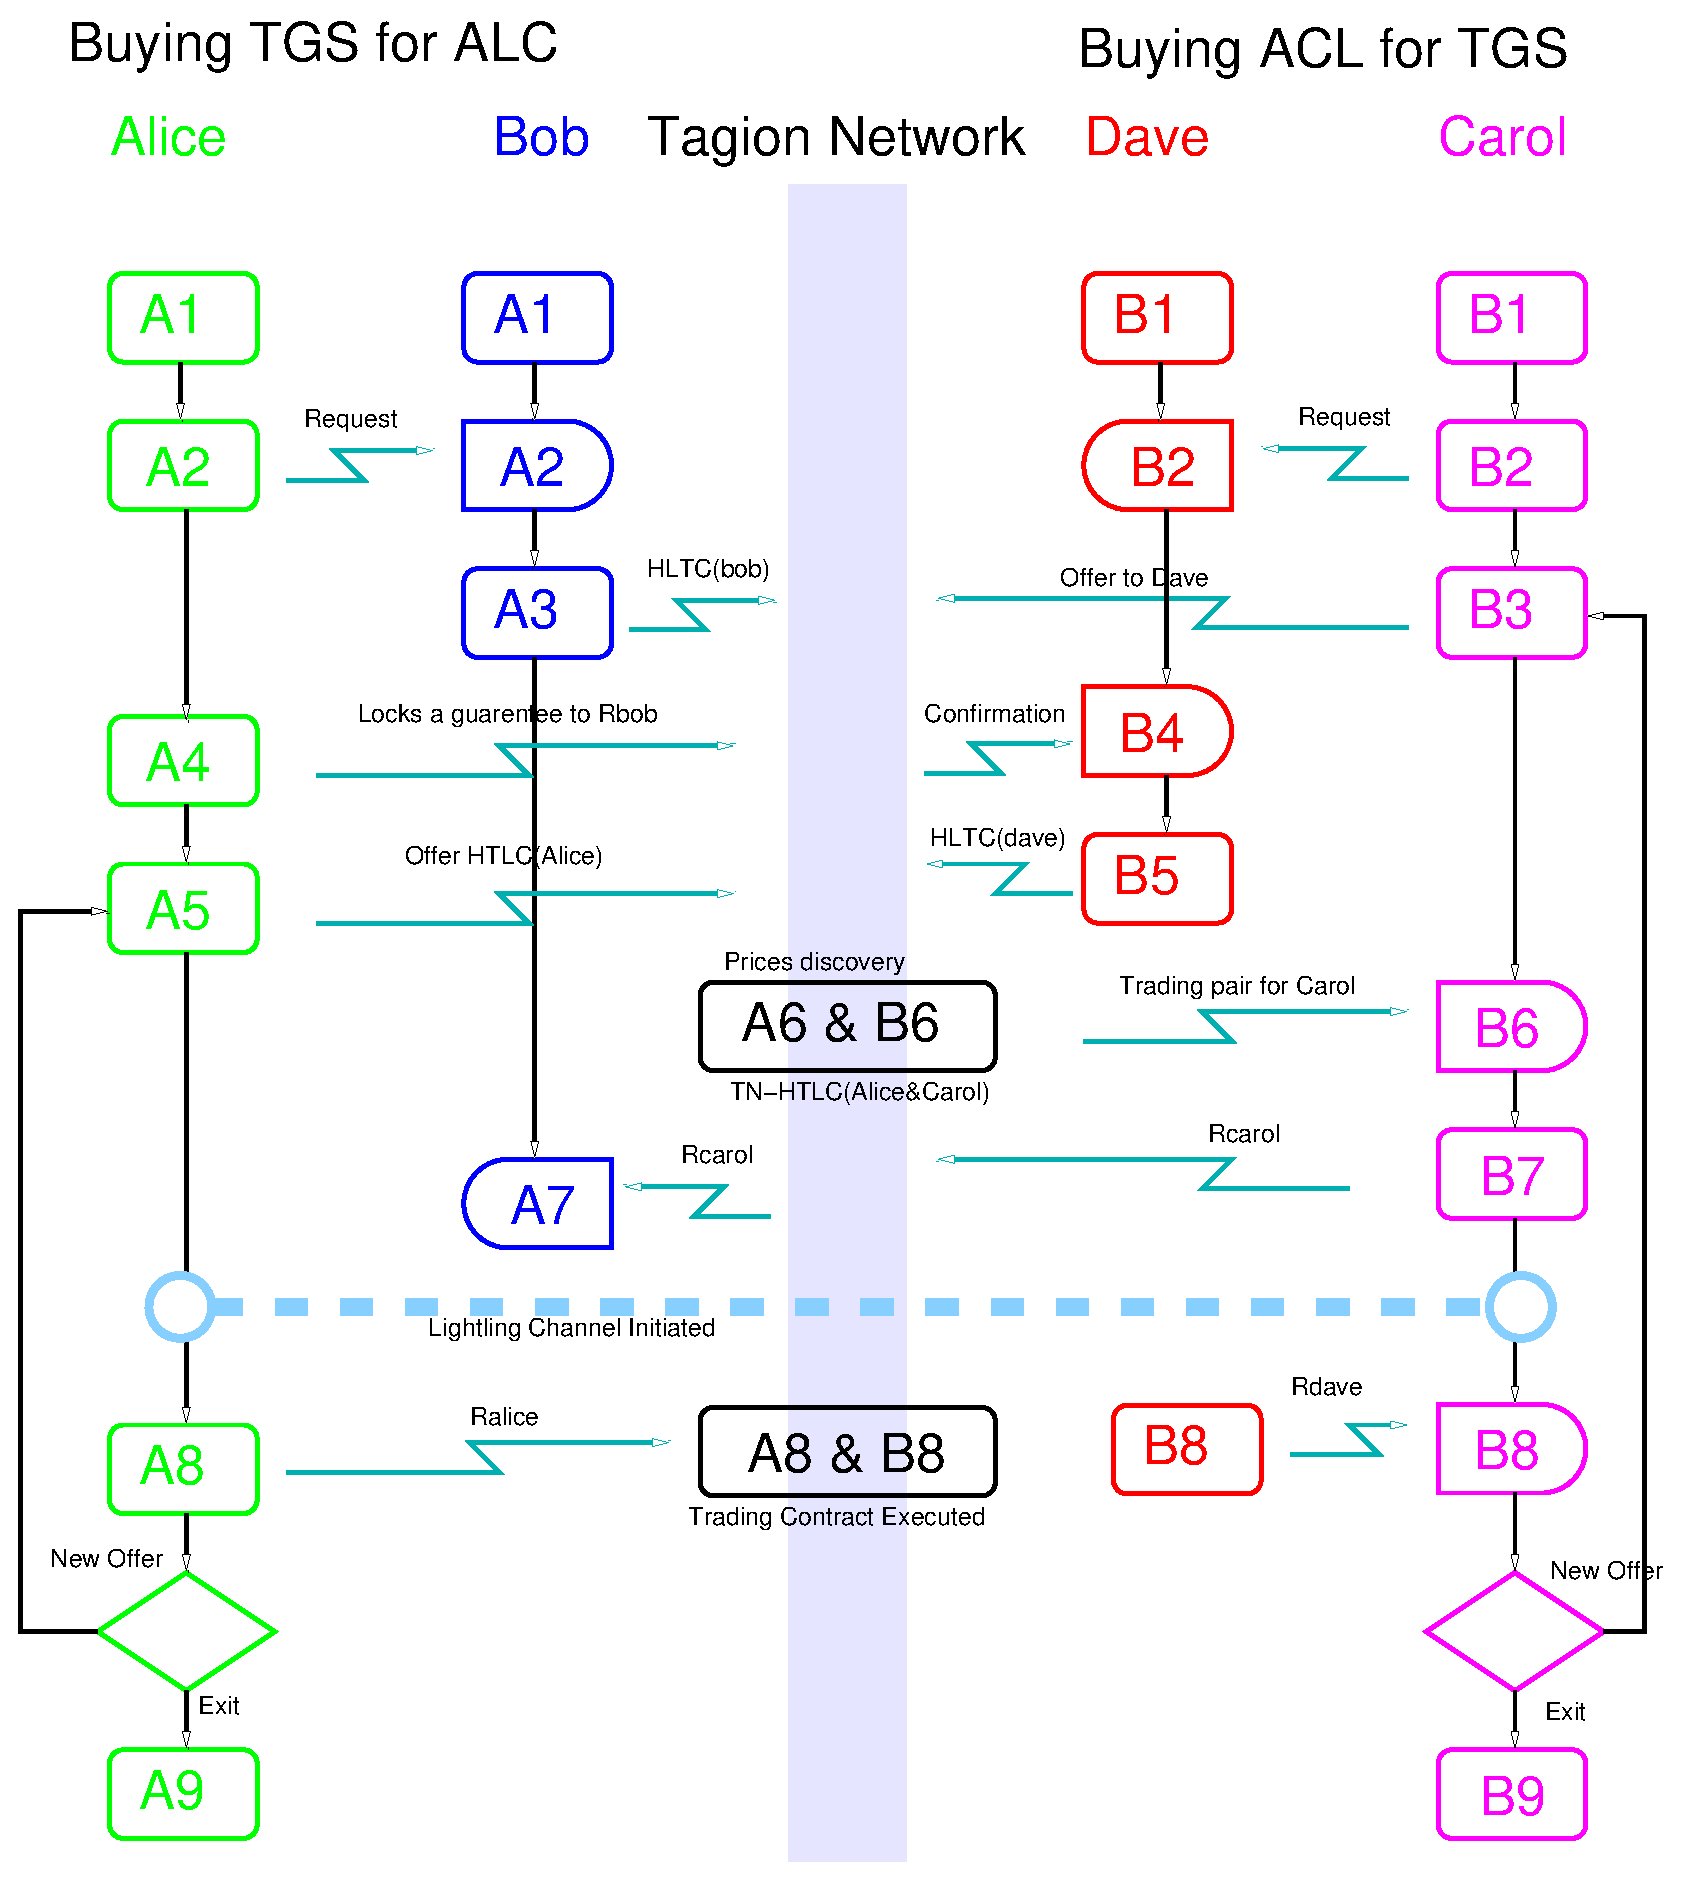
\includegraphics[width=1.0\textwidth]{fig/dex_flow.eps}
 \caption{DEX transaction flow}
 \label{fig:dex_flow}
\end{figure}

\paragraph{Incentives and Penalty}
If one or more of the 4 participants (Alice, Bob, Carol and Dave) fails to execute the trade, the flowing penalty rules will be performed by the TN consensus.
%\begin{enumerate}
\begin{enumerate}[\S 1]
\item \textbf{Alice doesn't claim the transaction} 
 \begin{description}
  \item \textbf{Incident} 
   \begin{itemize}
    \item 
    If Alice does not reveal $R_{alice}$ within the timeout limit.
   \end{itemize}
    \item \textbf{Action}
  \begin{itemize}
    \item 
    After a timeout period less than the Alice HLTC time lock.
    \item 
    The funds will be reverted to Carol.
    \item 
    The trade is deleted.
    \item 
    Bob keeps Alice's stacked fund's.
    \item 
    If the price of Alice's funds is less than Bob's guaranteed funds, Bob gets some of his funds back, which corresponds to the current trading prices.
    \item 
    The rest of Bob funds is burned.
    \item 
    If Alice reveals the $R_{alice}$ after the timeout, Alice loses her funds to Carol.
  \end{itemize}
 \end{description}
    \item \textbf{Bob doesn't initial the routing}
 \begin{description}
  \item \textbf{Incident}
   \begin{itemize}
    \item 
  If Bob is offline or choses not establish a connection within the a timeout period.
   \end{itemize}
  \item \textbf{Action}
   \begin{itemize}
    \item 
    Bob loses his funds and the trade bill is deleted.
    \item 
    Carol's funds are returned.
    \item 
    Alice will get her funds back after the HTLC time lock runs out.
   \end{itemize}
 \end{description}
 \item \textbf{Carol doesn't claim the transaction}
 \begin{description}
   \item \textbf{Incident} 
   \begin{itemize}
    \item 
    Carol does not reveal the $R_{carol}$ within the timeout limit.
   \end{itemize}
   \item \textbf{Action}
   \begin{itemize}
    \item 
    If Bob makes creates a contract which returns Alice's funds with a time limit Bob gets his funds back.
   \item
    Carol's transaction stake is burned and the rest of the funds is returned to Carol.
   \item
    The transactions bill is deleted.
   \end{itemize}
 \end{description} 
 \item \textbf{Dave doesn't accept the routing}
 \begin{description}
   \item \textbf{Incident} 
   \begin{itemize}
    \item 
    If Dave is offline or choses not establish connection within the a timeout period.
   \end{itemize}
   \item \textbf{Action}
   \begin{itemize}
    \item 
    After the timeout Carol can reclaim the stack $\omega_{carol}$ and open a new channel with Eric.
    \item
    Dave's stack $\omega_{dave}$ is burned
    \item
    Carol can initial the trade by revealing $R_{carol}$.
   \item
    The transaction's bill is deleted after execution.
   \end{itemize}
 \end{description} 
\end{enumerate}


%
% Appedix starts here
%
\appendix

\pagebreak
\pagenumbering{roman}
\section{HiBON Data format}
\label{sec:hibon}
All data exchanged and stored in the network is structured using a data format called \abbrev{HiBON}{Hash-invariant Binary Object Notation} which is inspired by \abbrev{BSON}{Binary JSON}, but the two formats are not compatible. In HiBON the keys are sorted according to the ordering rules described below (in D-lang). By ordering the keys, the data is hash invariant for the same collection.\\
%The algorithm use to order the key is shown below (D-lang):

\lstset{language=c++, numbers=left, numberstyle=\tiny, stepnumber=1, numbersep=5pt, tabsize=4}%, 
\begin{lstlisting}
@safe
bool less_than(string a, string b) pure
     in {
          assert(a.length > 0);
          assert(b.length > 0);
     }
body {
     static bool is_index(string a, out uint result) pure {
          import std.conv : to;
          enum MAX_UINT_SIZE=to!string(uint.max).length;
          if ( a.length <= MAX_UINT_SIZE ) {
               if ( a[0] == '0' ) {
                    return false;
               }
               foreach(c; a[1..$]) {
                    if ( (c < '0') || (c > '9') ) {
                         return false;
                    }
               }
               immutable number=a.to!ulong;
               if ( number <= uint.max ) {
                    result = cast(uint)number;
                    return true;
               }
          }
          return false;
     }
     uint a_index;
     uint b_index;
     if ( is_index(a, a_index) && is_index(b, b_index) ) {
          return a_index < b_index;
     }
     return a < b;
}
\end{lstlisting}

Only printable ASCII keys are allowed to be used as keys in the HiBON; this means no control characters or special characters allowed. The key is validated accordingly to the function described below.
\begin{lstlisting}
@safe bool is_key_valid(string a) pure nothrow {
     enum : char {
          SPACE = 0x20,
          DEL = 0x7F,
          DOUBLE_QUOTE = 34,
          QUOTE = 39,
          BACK_QUOTE = 0x60
              }
     if ( a.length > 0 ) {
          foreach(c; a) {
               // Chars between SPACE and DEL is valid
               // except for " ' ` is not valid
               if ( (c <= SPACE) || (c >= DEL) ||
                   ( c == DOUBLE_QUOTE ) || ( c == QUOTE ) ||
                   ( c == BACK_QUOTE ) ) {
                    return false;
               }
          }
          return true;
     }
     return false;
}
\end{lstlisting}


\begin{table}[H]
\begin{center}
\begin{tabular}{|p{3.5cm}|l|p{1.5cm}|p{8cm}|}
 %     \rowcolor{table_header_color}
      \hline
      Data type & Code & D-Type & Description \\
      \hline
      float64 & 0x01 & \texttt{double} & 64bit floating point \\
      \hline
      string & 0x02 & \texttt{string} & UTF-8 string \\
      \hline
      Embedded document & 0x03 & \texttt{\{\}} & HiBON object \\
      \hline
      Embedded array & 0x04 & \texttt{[]} & HiBON Array object (Only index numbers allowed) \\
      \hline
%      Binary data & 0x05 & -- & Binary in as sub-type \\
%      \hline
      Boolean & 0x08 & \texttt{bool} & Boolean false=0, true=1 \\
      \hline
      64bits UTC Time & 0x09 & \texttt{utc} & UTC datetime 64bits signed integer \\
      \hline
      int32 number & 0x10 & \texttt{int} & 32bit usigned number \\
      \hline
      int64 number & 0x12 & \texttt{long} & 64bits signed integer \\
      \hline
      float128 & 0x13 & \texttt{decimal} & 128bits floating point \\
      \hline
      Big integer & 0x18 & \texttt{bigint} & Signed big integer \\
      \hline
      uint32 & 0x20 & \texttt{uint} & 32bit unsigned number \\
      \hline
      float32 & 0x21 & \texttt{float} & 32bit floating point \\
      \hline
      uint64 & 0x22 & \texttt{ulong} & 64bit unsigned number \\
      \hline
      Big integer & 0x28 & \texttt{ubigint} & Unsigned big integer \\
      \hline
      Native Document  & 0x43 & \texttt{Document} & Reserved for internal use only \\
      \hline
      Defines Array    & 0x80 & \texttt{void} & Reserved type for internal use only \\
      \hline
      Array of float64 & 0x81 & \texttt{double[]} & Array of unsigned 64bits integer (size is multiple of 8bytes) \\
      \hline
      Binary string    & 0x85 & \texttt{ubyte[]} & Array of bytes (size is multiple of 1bytes)\\
      \hline
      Array of int32   & 0x90 & \texttt{int[]} & Array of 32bits signed integers (size is multiple of 4bytes) \\
      \hline
      Array of int64   & 0x92 & \texttt{long[]} &  Array of 64bits signed integer (size is multiple of 8bytes) \\
      \hline
      Array of int32 & 0x90 & \texttt{int[]} & Array of 32bits integer (size is multiple of 4bytes) \\
      \hline
      Array of uint64 & 0x92 & \texttt{long[]} & Array of 64bits integer (size is multiple of 8bytes) \\
      \hline
      Array of float128 & 0x93 & \texttt{decimal[]}  & Array of 128bits floating point (size is multiple of 16bytes) \\
      \hline
      Array of uint32 & 0xA0 & \texttt{uint[]} & Array of unsigned 32bits integer (size is multiple of 4bytes) \\
      \hline
      Array of float32 & 0xA1 & \texttt{float[]}  & Array of 32bits floating point (size is multiple of 4bytes) \\
      \hline
      Array of int64 & 0xA2 & \texttt{ulong[]} & Array of unsigned 64bits integer (size is multiple of 8bytes) \\
      \hline
      Defines string arrays    & 0x83 & \texttt{string[]} & Reserved type for internal use only \\
      \hline
      Defines Document arrays  & 0xC3 & \texttt{Document[]} & Reserved type for internal use only \\
      \hline
      Defines HiBON arrays     & 0x82 & \texttt{HiBON[]} & Reserved type for internal use only \\
      \hline
  \end{tabular}
\end{center}
\caption{HiBON Basic data-types}
\label{tab:hibon}
\end{table}


Any data types which are not defined in \cref{tab:hibon} are illegal and must be rejected by the network. The types used in the table are primarily the types used in D except for a few as \texttt{\{\}} and \texttt{[]}.

\subsection{HRPC – HiBON Remote Procedure Call}
HRPC works like JSON-RPC just with signed binary data, the above-defined HiBON format. It means the data is hash-invariant enabling hash- and signature functions to be executed quickly and unambiguously.

\begin{table}[H]
\begin{center}
\begin{tabular}{|l|p{7cm}|p{1.5cm}|l|}
      \hline
      Parameter & Description & Type & Access \\
      \hline
      $\$type$ & Set contract type to 'HRPC' &  \texttt{string} & \texttt{ro} \\
      \hline
      $\$pkey$ & Public key &  \texttt{bin} & \texttt{ro} \\
      \hline
      $\$sign$ & Signature of $\$msg$ &  \texttt{bin} & \texttt{ro} \\
      \hline
      $\$msg$ & Message object \cref{tab:HRPC_method_message}, \cref{tab:HRPC_success_message}, \cref{tab:HRPC_error_message} &  \texttt{\{\}} & \texttt{ro} \\
      \hline
  \end{tabular}
\end{center}
\caption{HRPC format} 
\label{tab:HRPC_format}
\end{table}

\begin{table}[H]
\begin{center}
\begin{tabular}{|l|p{7cm}|p{1.5cm}|l|}
      \hline
      Parameter & Description & Type & Access \\
      \hline
      $\$id$ & Message id  &  \texttt{uint} & \texttt{ro} \\
      \hline
      $\$method$ & Name of remote call function &  \texttt{string} & \texttt{ro} \\
      \hline
      $\$params$ & Params for the \$method function (optional) &  \texttt{\{\}} & \texttt{ro} \\
      \hline
  \end{tabular}
\end{center}
\caption{HRPC method message object} 
\label{tab:HRPC_method_message}
\end{table}

\begin{table}[H]
\begin{center}
\begin{tabular}{|l|p{7cm}|p{1.5cm}|l|}
      \hline
      Parameter & Description & Type & Access \\
      \hline
      $\$id$ & Message id &  \texttt{uint} & \texttt{ro} \\
      \hline
      $\$result$ & Result of the $\$method$ call &  \texttt{\{\}} & \texttt{ro} \\
      \hline
  \end{tabular}
\end{center}
\caption{HRPC success message object } 
\label{tab:HRPC_success_message}
\end{table}

\begin{table}[H]
\begin{center}
\begin{tabular}{|l|p{7cm}|p{1.5cm}|l|}
      \hline
      Parameter & Description & Type & Access \\
      \hline
      $\$id$ & Message id & \texttt{string} & \texttt{ro} \\
      \hline
      $\$msg$ & Error object \cref{tab:HRPC_error} & \texttt{\{\}} & \texttt{ro} \\
      \hline
  \end{tabular}
\end{center}
\caption{HPPC error response object } 
\label{tab:HRPC_error_message}
\end{table}


\begin{table}[H]
\begin{center}
\begin{tabular}{|l|p{7cm}|p{1.5cm}|l|}
      \hline
      Parameter & Description & Type & Access \\
      \hline
      $\$code$ & Set contract type to 'HRPC' & \texttt{uint} & \texttt{ro} \\
      \hline
      $\$msg$ & Error message  & \texttt{string} & \texttt{ro} \\
      \hline
      $\$data$ & Data object (optional) & \texttt{[]} & \texttt{ro} \\
      \hline
  \end{tabular}
\end{center}
\caption{HRPC error object } 
\label{tab:HRPC_error}
\end{table}


\pagebreak
\section{Crypto “Bank” bill}

The bill has a value $V$, public/private key $(y, x)$ and the bank bill number $B$, which is the hash of the bill.\\
V can have the value of a natural number: $V \in N$\\
This is a newly printed bill:
%\begin{equation}
\begin{align}
 Y_{alice} & = H ( L_{k+1} \parallel y_{alice} ) \\
 B_{k+1} & = H ( V \parallel L_{k+1} \parallel t_{k+1} \parallel T \parallel Y_{alice} )
\end{align}
%\end{equation}

($H$ is a hash function, is the hash of the previous confirmed Bull’s eye,  is the consensus timestamp of the current Epoch, is the epoch number and $T$ is the contact type) \\

The total value of all bills of type $T$ must be accounted for.
\begin{align}
 V_{total,k+1} & = V_{total,k+1} + V_{k} 
\end{align}


\paragraph{Simple transaction}
Ownership of the bill can be transferred to Bob, if:
\begin{itemize}
 \item 
    Bob reveals his public key to Alice 
 \item 
    Alice generates a new bill and signs it with her private key 
\end{itemize}


Because of the network fee, the value will be reduced by ${\Delta}V$.
\begin{equation}
 V_{k+1} = V_k - {\Delta}V
\end{equation}

If $V_{k+1}$ is negative or zero, the transaction is eliminated and will not generate a new bill.
\begin{equation}
 V_{total,k+1} = 
 \begin{cases}
  V_{total,k} - {\Delta}V & \text{if} ~ ( V_k - {\Delta}V \ge 0 ) \\
  V_{total,k} - V_k & \text{otherwise}     
 \end{cases}
\end{equation}


Resulting in:
\begin{equation}
 \begin{align*}
 Y_{bob} & = H(B_k \parallel y_{bob} ) \\
 B_{k+1} & = H ( V \parallel B_k \parallel t_k \parallel k \parallel T \parallel Y_{bob} )
\end{align*}
\end{equation}


The new bill is now written to the DART with key $B_{k+1}$:
\begin{equation*}
 V_{k+1}, B_k, t_k, k, T, Y_{bob} 
\end{equation*}


The old bill $B_k$  is removed from the DART. \\ 

The Split of a crypto bill \\
A bill can be split into a number of other bills if the combined value of the new nodes matches the original:
 \begin{equation}
  V_k = \left [ \sum_{i=0}^{I-1} {V_{k+1,i}} \right ] + {\Delta}V
 \end{equation}

Each new bill is generated as:
\begin{equation}
 \begin{align*}
 Y_{k+1,i} & = H ( B_k \parallel y_{k+1,i} ) \\
 B_{k+1,i} & = H ( V_{k+1} \parallel B_k \parallel t_k \parallel k \parallel T \parallel Y_{k+1} ), 
 ~ y_{k+1,i} \ne y_{k+1,j} ~ \text{for} ~ (i \ne j) \\
\end{align*}
\end{equation}
 

All new bills marked $B_{k+1}$ are stored in the DART as before, and the old bills are removed. \\
Join or collect bills into one bill.\\
A number of bills can be collated into one bill if the value adds up as follows:
\begin{equation}
 V_a = \left[ \sum_{i=0}^{I-1} {V_{b,i}} \right] + {\Delta}V    
\end{equation}

The new common bill number is generated by hashing a sorted list of the joined bill numbers.  
\begin{equation}
 B'_k = H ( B_{k,0} \parallel B_{k,1} ... \parallel B_{k,I-1} )
\end{equation}

The new bill number will be generated: 
\begin{equation}
 \begin{align*}
  Y'_{k+1} & = H ( B'_k \parallel y_{k+1} ) \\
  B_{k+1} & = H ( V_a \parallel B'_k \parallel t_k \parallel k \parallel T \parallel Y'_{k+1} ) \\
 \end{align*}
\end{equation}

These new consolidated bills are stored in the DART.


\pagebreak
\section{Network}\label{sec:network}
The following steps are executed in the network for a standard transaction:
\begin{enumerate}
 \item 
     The transaction object is sent to one of the active nodes (an inactive node should relay the transaction object to an active node).
 \item 
    When a node receives a transaction object, its format and the signatures of all the inputs are checked.
 \item 
    If the transaction object is valid, it is added to the payload of an event.
 \item 
    The event is gossiped to the network.
 \item 
    The payload is put into an epoch list in order.
 \item 
    The epoch list is processed in the epoch order.
 \item 
    All inputs to the transaction are collected from the DART database.
 \item 
    The transaction script is executed when all inputs are read from the DART.
 \item 
    The output of the transaction scripts is gossiped to the network.
 \item 
    When the network reaches consensus on all outputs of the transactions, the DART is updated. 
 \item 
    The new Merkle root (Bull’s eye) of the DART is calculated, and the Bull’s eye is gossiped to the network. 
 \item 
    When the majority of the nodes reach consensus on the Bull’s eye, it is added to the DART blockchain. The transaction is now approved.
\end{enumerate}


\pagebreak
\section{Network Security}
\paragraph{Network attack surface\\} 
In the following, the probability of an evil attack on the network is estimated via a simple model. \\
The network participants are given by the flowing parameters.\\
\begin{itemize}
 \item[$M$] is the total number of nodes which are available for the network (This includes active and passive nodes, not prospect nodes). 
\item[$N$] is the number of active nodes running the networks. 
\item[$E$] is the number of nodes controlled by the evil attacker. 
\item[$n_E$] is the number of evil nodes among the $N$ active nodes. 
 \end{itemize}

The attack scenario is divided into two categories. The first category prevents the network from reaching a consensus, and in the second category, the attacker is able to take over the network and decide the faith what is going which transactions going it to a block. \\
\paragraph{First category:\\}
If the evil attacker wants to prevent the networks from reaching a consensus, the evil attacker needs more than $1/3$ of the active nodes.
\begin{equation}
 \frac{n_E}{N} > \frac{1}{3}
\end{equation}

\paragraph{Second category:\\}
If the evil attacker wants to take over the network, the attacker needs more than $2/3$ of the active nodes.
\begin{equation}
 \frac{n_E}{N} > \frac{2}{3}
\end{equation}


The calculated scenario is based on all the $N$ nodes being changed at every epoch. In the real network, this is not the case; only one node is swapped out and in at every $100$ epoch. Thus the probability of an evil takeover is significantly lower than this calculation. The model is chosen because it is easy to express mathematically. 
The active nodes are selected randomly from $M$, and the probability that the evil attacker controls the first selected node is:\\

Definition of permutation formula:
\begin{equation}
 P(n,r) = \frac{n!}{(n-r)!}
\end{equation}

Definition of combination formula:
\begin{equation}
 C(n,r) = \frac{n!}{(n-r)! \cdot r!} = \frac{P(n,r)}{r!}
\end{equation}


The probability of an evil node being selected is:
\begin{equation}
 p_{E_0} = \frac{E}{M}
\end{equation}

The probability of selecting an evil node after selecting an evil node at the nth time is:
\begin{equation}
 p_{E_n} = \frac{E-n}{M-n}
\end{equation}


The probability of constructing an evil network\\
In this section, the probability of constructing an evil network is calculated.\\
The network is randomly constructed by selecting $N$ nodes out of $M$ nodes where $E$ nodes are evil.\\
A network is defined to be evil if the network contains $n_E$ or more evil nodes out of the $N$ active nodes according to formula first and second category formula above.\\

The probability that $n_E$ nodes out of $N$ nodes are:
\begin{equation}
 p_{E_n} = \left. \prod_{i=0}^{n_E-1}{p_{E_i}} \cdot \prod_{i=n_E}^{N_E}{(1-p_{E_i}) \cdot C(N,n_E)} \right| _{N_E = min(E,N)}
\end{equation}


If $M \gg n_E$  and $E \gg n_E$  the probability can be approximated to:
\begin{equation}
 p_{n_E} \approx p_{E_0}^{n_E} \cdot (1-p_{E_0})^{N-n_E} \cdot C(N,n_E) ~ \text{for} ~ \frac{E}{M} \approx \frac{E-n_E}{M-n_E}
\end{equation}

The probability that $n_E$ nodes or more are:
\begin{equation}
 p_{n>n_E} = \left. \sum_{i=N_E}{n_E}{p_i \cdot C(N,i)} \right|_{N_E = min(E,N)}
\end{equation}


Example if $N=100$ and $M=1000$ and the attacker has $E$ nodes, the probability that the attacker can prevent the network from reaching a consensus is:
\begin{align*}
 M &= 200 & M &= 1000 & M &= 10000 \\
 N &= 60 & N &= 100 & N &= 100 \\
 E &= 60 & E &= 100 & E &= 500 \\
 n_E &= 21 & n_E &= 34 & n_E &= 34 \\
 p_{n \ge 20 } &= 0.199261 & p_{n \ge 34} &= 1.62609 \cdot 10^{-12} & p_{n \ge 34} &= 5.24507 \cdot 10^{-20}
\end{align*}

For an attacker to take over the network:
\begin{align*}
 M &= 200 & M &= 1000 & M &= 10000 \\
 N &= 60 & N &= 100 & N &= 100 \\
 E &= 60 & E &= 100 & E &= 500 \\
 n_E &= 41 & n_E &= 67 & n_E &= 67 \\
 p_{n \ge 41 } &= 4.2687 \cdot 10^{-14} & p_{n \ge 67} &= 9.34035 \cdot 10^{-54} & p_{n \ge 67} &= 5.68532 \cdot 10^{-64}
\end{align*}


If we have an epoch time of $10$ seconds and the probability is $10^{-53}$ then the evil attacker can take over the network every $10^{46}$ years or around $10^{36}$ the current age of the universe.

Note.
For a very large number of $M$ and $N$ the probability can be expressed as a logarithm formula to prevent numerical overflow.\\
Combination expressed as a logarithm formula:
%\begin{equation}
\begin{align*}
 \Phi (n,r) &= \sum_{k=r+1}^{n}{ln(k)} - \sum_{k=1}^{r}{ln(k)} \\
 C(n,r) &= e^{{\Phi}(n,r)}
\end{align*}
%\end{equation}


The probability expresses as a logarithm:

%\begin{equation}
\begin{align*}
{\Pi}_{E_n} &= \left. \left( \sum_{i=0}^{n_E-1}{ln(p_{E_i})} - \sum_{i=n_E}^{N_E}{ln(1-p_{E_i})} \right) 
\right|_{N_E = min(E,N)} \\
p_{E_n} &= e^{({\Pi}_{E_n}+\Phi(N,n_E))}
\end{align*}
%\end{equation}


If $M \gg n_E$ and $E \gg n_E$ the probability can be approximated to:
%\begin{equation}
\begin{align*}
 p_{E_n} & \approx e^{(n_E \cdot ln(p_{E_0})-(N_E-n_E) \cdot (1-ln(P_{E_0})+\Phi(N,n_E)))} \\ 
         &\approx e^{((2 \cdot n_E - N_E) \cdot ln(p_{E_0}) + n_E - N_E + \Phi(N,n_E))} ~ 
 \text{for} ~ \frac{E}{M} \approx \frac{E-n_E}{M-n_E}
\
\end{align*}
%\end{equation}

\paragraph{Security conclusion\\}
By having a volume of, e.g. $1000$ nodes and $100$ active nodes, which could be a possible amount for a network or shard, then the probability is so low that it will probably never occur in practice. Thus, the actual security is that the nodes are decentralised. Therefore, the node governance protocol is the actual security mechanism, because it regulates the uptake of nodes aiming for it to be democratic, meaning both decentralised and one physical person having only one node.  


\pagebreak
\section{Consensus Probability}

\paragraph{Epoch consensus}
In the following the probability for the Hashgraph-algorithm to reach an Epoch consensus within $H$ events consecutive is estimated in a simple model as follows.\\

The network participants are given by the flowing parameters.
\begin{itemize}
	\item[$H$] is the number of event for a node to reach Epoch-consensus.
	\item[$M$] is the total number of nodes which are available for the network (This includes active and passive nodes, not prospect nodes). 
	\item[$n$] is the number of nodes which has not yet been seen by the current node. 
\end{itemize}

The probability for a node to gossip to another node which has not yet been seen:
\begin{equation}
P_{n} = \frac{M-n}{M}
\end{equation}

The number $H$ is define as more than $2/3$ of the number $M$.

\begin{equation}
H = floor \left( \frac{2}{3} M \right)
\end{equation}

The probability for gossip $h$ different nodes in $h$ consecutive events can calculated as:
\begin{equation}
P_{h,0} = \prod _{n=1}^{h} P_n
\end{equation}


The probability for gossip $h$ different nodes in $h+1$ consecutive events can calculated as:
\begin{equation}
P_{h,i} = \sum_{i=0}^{N-1} \prod _{n=1}^{h+1} P_n
\end{equation}

A binary vector $S_{h,H}$ is defined as follow:

\begin{align}
S_{h,H} = [b_{0}, b_{1} .. b_{h-1}] ~ b_{i} \in \mathbb{B}\\
\text{where}\\
\sum S_{h,H} = H
\end{align}




\begin{equation}
P(n,r) = \frac{n!}{(n-r)!}
\end{equation}


\pagebreak
\section{DEX Trading Example}\label{sec:dex_example}

An example of the DEX matching and prices-discovery algorithm described in \cref{sec:dex} is shown in the following tables. The trading-order-queue in \cref{tab:trading_order_queue} and the two sorted sales list are generated and shown in \cref{tab:ask_sales_list} and \cref{tab:bid_sales_list}.

\begin{table}[H]
\begin{center}
\begin{tabular}{|r|c|r|r|r|r|r|p{2cm}|p{2cm}|r|}
\hline

No & Type & Size & $P$ & $Q$ & $E_{ask}$ & $E_{bid}$ & Bought & Sold & Id \\
\hline
0 & ATO & 83TGS & 147 & 10 & 0.0680 & 14.7000 &    &    &    \\
\hline
1 & ATO & 6TGS & 138 & 12 & 0.0870 & 11.5000 &    &    &    \\
\hline
2 & BTO & 785ACL & 116 & 10 & 0.0862 & 11.6000 &    &    &    \\
\hline
3 & ATO & 79TGS & 149 & 10 & 0.0671 & 14.9000 &    &    &    \\
\hline
4 & ATO & 4TGS & 113 & 10 & 0.0885 & 11.3000 &    &    &    \\
\hline
5 & BTO & 217ACL & 145 & 11 & 0.0759 & 13.1818 &    &    &    \\
\hline
6 & BTO & 936ACL & 115 & 13 & 0.1130 & 8.8462 &    &    &    \\
\hline
7 & BTO & 205ACL & 145 & 11 & 0.0759 & 13.1818 &    &    &    \\
\hline
8 & BTO & 949ACL & 146 & 10 & 0.0685 & 14.6000 &    &    &    \\
\hline
9 & BTO & 888ACL & 117 & 10 & 0.0855 & 11.7000 &    &    &    \\
\hline
10 & BTO & 587ACL & 112 & 10 & 0.0893 & 11.2000 &    &    &    \\
\hline
11 & BTO & 314ACL & 126 & 13 & 0.1032 & 9.6923 &    &    &    \\
\hline
12 & BTO & 503ACL & 118 & 12 & 0.1017 & 9.8333 &    &    &    \\
\hline
13 & ATO & 72TGS & 106 & 12 & 0.1132 & 8.8333 &    &    &    \\
\hline
14 & ATO & 57TGS & 108 & 13 & 0.1204 & 8.3077 &    &    &    \\
\hline
15 & BTO & 341ACL & 131 & 12 & 0.0916 & 10.9167 &    &    &    \\
\hline
16 & ATO & 15TGS & 127 & 10 & 0.0787 & 12.7000 &    &    &    \\
\hline
17 & ATO & 43TGS & 111 & 11 & 0.0991 & 10.0909 &    &    &    \\
\hline
18 & BTO & 85ACL & 136 & 12 & 0.0882 & 11.3333 &    &    &    \\
\hline
19 & ATO & 29TGS & 144 & 10 & 0.0694 & 14.4000 &    &    &    \\
\hline
20 & ATO & 63TGS & 144 & 14 & 0.0972 & 10.2857 &    &    &    \\
\hline
21 & BTO & 716ACL & 134 & 11 & 0.0821 & 12.1818 &    &    &    \\
\hline
22 & ATO & 42TGS & 139 & 12 & 0.0863 & 11.5833 &    &    &    \\
\hline
23 & ATO & 37TGS & 114 & 13 & 0.1140 & 8.7692 &    &    &    \\
\hline
24 & ATO & 45TGS & 136 & 10 & 0.0735 & 13.6000 &    &    &    \\
\hline
25 & ATO & 44TGS & 131 & 12 & 0.0916 & 10.9167 &    &    &    \\
\hline
26 & BTO & 87ACL & 134 & 10 & 0.0746 & 13.4000 &    &    &    \\
\hline
27 & BTO & 739ACL & 146 & 13 & 0.0890 & 11.2308 &    &    &    \\
\hline
28 & ATO & 16TGS & 138 & 14 & 0.1014 & 9.8571 &    &    &    \\
\hline
29 & ATO & 42TGS & 104 & 10 & 0.0962 & 10.4000 &    &    &    \\
\hline
30 & ATO & 79TGS & 101 & 12 & 0.1188 & 8.4167 &    &    &    \\
\hline
31 & BTO & 725ACL & 117 & 13 & 0.1111 & 9.0000 &    &    &    \\
\hline
32 & ATO & 3TGS & 144 & 13 & 0.0903 & 11.0769 &    &    &    \\
\hline
33 & BTO & 226ACL & 144 & 12 & 0.0833 & 12.0000 &    &    &    \\
\hline
34 & ATO & 30TGS & 140 & 13 & 0.0929 & 10.7692 &    &    &    \\
\hline
35 & BTO & 526ACL & 131 & 14 & 0.1069 & 9.3571 &    &    &    \\
\hline
\end{tabular}

\end{center}
\caption{DEX Trading-order-queue} 
\label{tab:trading_order_queue}
\end{table}

\pagebreak
\begin{table}[H]
\begin{center}
\begin{tabular}{|r|c|r|r|r|r|r|p{2cm}|p{2cm}|r|}
\hline

No & Type & Size & $P$ & $Q$ & $E_{ask}$ & $E_{bid}$ & Bought & Sold & Id \\
\hline
14 & ATO & 57TGS & 108 & 13 & 0.1204 & 8.3077 &    &    &    \\
\hline
30 & ATO & 79TGS & 101 & 12 & 0.1188 & 8.4167 &    &    &    \\
\hline
23 & ATO & 37TGS & 114 & 13 & 0.1140 & 8.7692 &    &    &    \\
\hline
13 & ATO & 72TGS & 106 & 12 & 0.1132 & 8.8333 &    &    &    \\
\hline
28 & ATO & 16TGS & 138 & 14 & 0.1014 & 9.8571 &    &    &    \\
\hline
17 & ATO & 43TGS & 111 & 11 & 0.0991 & 10.0909 &    &    &    \\
\hline
20 & ATO & 63TGS & 144 & 14 & 0.0972 & 10.2857 &    &    &    \\
\hline
29 & ATO & 42TGS & 104 & 10 & 0.0962 & 10.4000 &    &    &    \\
\hline
34 & ATO & 30TGS & 140 & 13 & 0.0929 & 10.7692 &    &    &    \\
\hline
25 & ATO & 44TGS & 131 & 12 & 0.0916 & 10.9167 &    &    &    \\
\hline
32 & ATO & 3TGS & 144 & 13 & 0.0903 & 11.0769 &    &    &    \\
\hline
4 & ATO & 4TGS & 113 & 10 & 0.0885 & 11.3000 &    &    &    \\
\hline
1 & ATO & 6TGS & 138 & 12 & 0.0870 & 11.5000 &    &    &    \\
\hline
22 & ATO & 42TGS & 139 & 12 & 0.0863 & 11.5833 &    &    &    \\
\hline
16 & ATO & 15TGS & 127 & 10 & 0.0787 & 12.7000 &    &    &    \\
\hline
24 & ATO & 45TGS & 136 & 10 & 0.0735 & 13.6000 &    &    &    \\
\hline
19 & ATO & 29TGS & 144 & 10 & 0.0694 & 14.4000 &    &    &    \\
\hline
0 & ATO & 83TGS & 147 & 10 & 0.0680 & 14.7000 &    &    &    \\
\hline
3 & ATO & 79TGS & 149 & 10 & 0.0671 & 14.9000 &    &    &    \\
\hline
\end{tabular}

\end{center}
\caption{Sort list of ATO or the ask-sales list} 
\label{tab:ask_sales_list}
\end{table}

%\pagebreak
\begin{table}[H]
\begin{center}
\begin{tabular}{|r|c|r|r|r|r|r|p{2cm}|p{2cm}|r|}
\hline

No & Type & Size & $P$ & $Q$ & $E_{ask}$ & $E_{bid}$ & Bought & Sold & Id \\
\hline
8 & BTO & 949ACL & 146 & 10 & 0.0685 & 14.6000 &    &    &    \\
\hline
26 & BTO & 87ACL & 134 & 10 & 0.0746 & 13.4000 &    &    &    \\
\hline
5 & BTO & 217ACL & 145 & 11 & 0.0759 & 13.1818 &    &    &    \\
\hline
7 & BTO & 205ACL & 145 & 11 & 0.0759 & 13.1818 &    &    &    \\
\hline
21 & BTO & 716ACL & 134 & 11 & 0.0821 & 12.1818 &    &    &    \\
\hline
33 & BTO & 226ACL & 144 & 12 & 0.0833 & 12.0000 &    &    &    \\
\hline
9 & BTO & 888ACL & 117 & 10 & 0.0855 & 11.7000 &    &    &    \\
\hline
2 & BTO & 785ACL & 116 & 10 & 0.0862 & 11.6000 &    &    &    \\
\hline
18 & BTO & 85ACL & 136 & 12 & 0.0882 & 11.3333 &    &    &    \\
\hline
27 & BTO & 739ACL & 146 & 13 & 0.0890 & 11.2308 &    &    &    \\
\hline
10 & BTO & 587ACL & 112 & 10 & 0.0893 & 11.2000 &    &    &    \\
\hline
15 & BTO & 341ACL & 131 & 12 & 0.0916 & 10.9167 &    &    &    \\
\hline
12 & BTO & 503ACL & 118 & 12 & 0.1017 & 9.8333 &    &    &    \\
\hline
11 & BTO & 314ACL & 126 & 13 & 0.1032 & 9.6923 &    &    &    \\
\hline
35 & BTO & 526ACL & 131 & 14 & 0.1069 & 9.3571 &    &    &    \\
\hline
31 & BTO & 725ACL & 117 & 13 & 0.1111 & 9.0000 &    &    &    \\
\hline
6 & BTO & 936ACL & 115 & 13 & 0.1130 & 8.8462 &    &    &    \\
\hline
\end{tabular}

\end{center}
\caption{Sort list of BTO or the bid-sales list} 
\label{tab:bid_sales_list}
\end{table}

\pagebreak
\subsection{DEX After the Trading Match}
The trade is executed from the first order in the queue which is the top of the \cref{tab:trading_order_queue} and the matching pairs shown in \cref{tab:matching_pairs}. A BTO order from the \cref{tab:trading_order_queue} is searched in \cref{tab:ask_sales_list} to see if $E_{bid,BTO} \geq E_{bid,ATO}$ and if the order is an ATO the \cref{tab:bid_sales_list} is searched and if $E_{ask,ATO} \geq E_{ask,BTO}$ a match is found. 
The executed trading-orders are shown in \cref{tab:trading_order_queue_executed} and the orders which remain are shown in \cref{tab:trading_order_queue_rest}.
The parameter \bfit{Id} shown in the tables, represents the execution order and matching \bfit{Id} of the trading pairs and \bfit{No} is the priority order in the trading-order-queue.

\begin{table}[H]
\begin{center}
\begin{tabular}{|c|c|c|c|c|c|c|c|c|c|}
\hline

Buyer $\rightarrow$ Seller & No $\rightarrow$ No & $E_{buyer}$ & $E_{seller}$ & Bought & Sold & Id \\
\hline
ATO$\rightarrow$BTO & 1$\rightarrow$8 & 0.0870 & 0.0685 & 6.00TGS & 87.60ACL & 1 \\
\hline
BTO$\rightarrow$ATO & 2$\rightarrow$14 & 11.6000 & 8.3077 & 473.54ACL & 57.00TGS & 2 \\
\hline
ATO$\rightarrow$BTO & 4$\rightarrow$26 & 0.0885 & 0.0746 & 4.00TGS & 53.60ACL & 3 \\
\hline
BTO$\rightarrow$ATO & 5$\rightarrow$30 & 13.1818 & 8.4167 & 217.00ACL & 25.78TGS & 4 \\
\hline
BTO$\rightarrow$ATO & 6$\rightarrow$23 & 8.8462 & 8.7692 & 324.46ACL & 37.00TGS & 5 \\
\hline
BTO$\rightarrow$ATO & 7$\rightarrow$13 & 13.1818 & 8.8333 & 205.00ACL & 23.21TGS & 6 \\
\hline
BTO$\rightarrow$ATO & 9$\rightarrow$28 & 11.7000 & 9.8571 & 157.71ACL & 16.00TGS & 7 \\
\hline
BTO$\rightarrow$ATO & 10$\rightarrow$17 & 11.2000 & 10.0909 & 433.91ACL & 43.00TGS & 8 \\
\hline
BTO$\rightarrow$ATO & 15$\rightarrow$20 & 10.9167 & 10.2857 & 341.00ACL & 33.15TGS & 9 \\
\hline
BTO$\rightarrow$ATO & 18$\rightarrow$29 & 11.3333 & 10.4000 & 85.00ACL & 8.17TGS & 10 \\
\hline
BTO$\rightarrow$ATO & 21$\rightarrow$34 & 12.1818 & 10.7692 & 323.08ACL & 30.00TGS & 11 \\
\hline
ATO$\rightarrow$BTO & 22$\rightarrow$33 & 0.0863 & 0.0833 & 18.83TGS & 226.00ACL & 12 \\
\hline
ATO$\rightarrow$BTO & 25$\rightarrow$27 & 0.0916 & 0.0890 & 44.00TGS & 494.15ACL & 13 \\
\hline
\end{tabular}

\end{center}
\caption{List of the matching pairs} 
\label{tab:matching_pairs}
\end{table}

%\pagebreak
\begin{table}[H]
\begin{center}
\begin{tabular}{|r|c|r|r|r|r|r|p{2cm}|p{2cm}|r|}
\hline

No & Type & Size & $P$ & $Q$ & $E_{ask}$ & $E_{bid}$ & Bought & Sold & Id \\
\hline
1 & ATO & 6TGS & 138 & 12 & 0.0870 & 11.5000 & 6.00TGS &    & 1 \\
\hline
2 & BTO & 785ACL & 116 & 10 & 0.0862 & 11.6000 & 473.54ACL &    & 2 \\
\hline
4 & ATO & 4TGS & 113 & 10 & 0.0885 & 11.3000 & 4.00TGS &    & 3 \\
\hline
5 & BTO & 217ACL & 145 & 11 & 0.0759 & 13.1818 & 217.00ACL &    & 4 \\
\hline
6 & BTO & 936ACL & 115 & 13 & 0.1130 & 8.8462 & 324.46ACL &    & 5 \\
\hline
7 & BTO & 205ACL & 145 & 11 & 0.0759 & 13.1818 & 205.00ACL &    & 6 \\
\hline
8 & BTO & 949ACL & 146 & 10 & 0.0685 & 14.6000 &    & 87.60ACL & 1 \\
\hline
9 & BTO & 888ACL & 117 & 10 & 0.0855 & 11.7000 & 157.71ACL &    & 7 \\
\hline
10 & BTO & 587ACL & 112 & 10 & 0.0893 & 11.2000 & 433.91ACL &    & 8 \\
\hline
13 & ATO & 72TGS & 106 & 12 & 0.1132 & 8.8333 &    & 23.21TGS & 6 \\
\hline
14 & ATO & 57TGS & 108 & 13 & 0.1204 & 8.3077 &    & 57.00TGS & 2 \\
\hline
15 & BTO & 341ACL & 131 & 12 & 0.0916 & 10.9167 & 341.00ACL &    & 9 \\
\hline
17 & ATO & 43TGS & 111 & 11 & 0.0991 & 10.0909 &    & 43.00TGS & 8 \\
\hline
18 & BTO & 85ACL & 136 & 12 & 0.0882 & 11.3333 & 85.00ACL &    & 10 \\
\hline
20 & ATO & 63TGS & 144 & 14 & 0.0972 & 10.2857 &    & 33.15TGS & 9 \\
\hline
21 & BTO & 716ACL & 134 & 11 & 0.0821 & 12.1818 & 323.08ACL &    & 11 \\
\hline
22 & ATO & 42TGS & 139 & 12 & 0.0863 & 11.5833 & 18.83TGS &    & 12 \\
\hline
23 & ATO & 37TGS & 114 & 13 & 0.1140 & 8.7692 &    & 37.00TGS & 5 \\
\hline
25 & ATO & 44TGS & 131 & 12 & 0.0916 & 10.9167 & 44.00TGS &    & 13 \\
\hline
26 & BTO & 87ACL & 134 & 10 & 0.0746 & 13.4000 &    & 53.60ACL & 3 \\
\hline
27 & BTO & 739ACL & 146 & 13 & 0.0890 & 11.2308 &    & 494.15ACL & 13 \\
\hline
28 & ATO & 16TGS & 138 & 14 & 0.1014 & 9.8571 &    & 16.00TGS & 7 \\
\hline
29 & ATO & 42TGS & 104 & 10 & 0.0962 & 10.4000 &    & 8.17TGS & 10 \\
\hline
30 & ATO & 79TGS & 101 & 12 & 0.1188 & 8.4167 &    & 25.78TGS & 4 \\
\hline
33 & BTO & 226ACL & 144 & 12 & 0.0833 & 12.0000 &    & 226.00ACL & 12 \\
\hline
34 & ATO & 30TGS & 140 & 13 & 0.0929 & 10.7692 &    & 30.00TGS & 11 \\
\hline
\end{tabular}

\end{center}
\caption{Orders which are matched and executed} 
\label{tab:trading_order_queue_executed}
\end{table}

\pagebreak
\begin{table}[H]
\begin{center}
\begin{tabular}{|r|c|r|r|r|r|r|p{2cm}|p{2cm}|r|}
\hline

No & Type & Size & $P$ & $Q$ & $E_{ask}$ & $E_{bid}$ & Bought & Sold & Id \\
\hline
14 & ATO & 57TGS & 108 & 13 & 0.1204 & 8.3077 &    & 57.00TGS & 2 \\
\hline
30 & ATO & 79TGS & 101 & 12 & 0.1188 & 8.4167 &    & 25.78TGS & 4 \\
\hline
23 & ATO & 37TGS & 114 & 13 & 0.1140 & 8.7692 &    & 37.00TGS & 5 \\
\hline
13 & ATO & 72TGS & 106 & 12 & 0.1132 & 8.8333 &    & 23.21TGS & 6 \\
\hline
28 & ATO & 16TGS & 138 & 14 & 0.1014 & 9.8571 &    & 16.00TGS & 7 \\
\hline
17 & ATO & 43TGS & 111 & 11 & 0.0991 & 10.0909 &    & 43.00TGS & 8 \\
\hline
20 & ATO & 63TGS & 144 & 14 & 0.0972 & 10.2857 &    & 33.15TGS & 9 \\
\hline
29 & ATO & 42TGS & 104 & 10 & 0.0962 & 10.4000 &    & 8.17TGS & 10 \\
\hline
34 & ATO & 30TGS & 140 & 13 & 0.0929 & 10.7692 &    & 30.00TGS & 11 \\
\hline
25 & ATO & 44TGS & 131 & 12 & 0.0916 & 10.9167 & 44.00TGS &    & 13 \\
\hline
4 & ATO & 4TGS & 113 & 10 & 0.0885 & 11.3000 & 4.00TGS &    & 3 \\
\hline
1 & ATO & 6TGS & 138 & 12 & 0.0870 & 11.5000 & 6.00TGS &    & 1 \\
\hline
22 & ATO & 42TGS & 139 & 12 & 0.0863 & 11.5833 & 18.83TGS &    & 12 \\
\hline
\end{tabular}

\end{center}
\caption{Sort list of ATO which are executed} 
\label{tab:ask_sales_list_executed}
\end{table}

%\pagebreak
\begin{table}[H]
\begin{center}
\begin{tabular}{|r|c|r|r|r|r|r|p{2cm}|p{2cm}|r|}
\hline

No & Type & Size & $P$ & $Q$ & $E_{ask}$ & $E_{bid}$ & Bought & Sold & Id \\
\hline
8 & BTO & 949ACL & 146 & 10 & 0.0685 & 14.6000 &    & 87.60ACL & 1 \\
\hline
26 & BTO & 87ACL & 134 & 10 & 0.0746 & 13.4000 &    & 53.60ACL & 3 \\
\hline
7 & BTO & 205ACL & 145 & 11 & 0.0759 & 13.1818 & 205.00ACL &    & 6 \\
\hline
5 & BTO & 217ACL & 145 & 11 & 0.0759 & 13.1818 & 217.00ACL &    & 4 \\
\hline
21 & BTO & 716ACL & 134 & 11 & 0.0821 & 12.1818 & 323.08ACL &    & 11 \\
\hline
33 & BTO & 226ACL & 144 & 12 & 0.0833 & 12.0000 &    & 226.00ACL & 12 \\
\hline
9 & BTO & 888ACL & 117 & 10 & 0.0855 & 11.7000 & 157.71ACL &    & 7 \\
\hline
2 & BTO & 785ACL & 116 & 10 & 0.0862 & 11.6000 & 473.54ACL &    & 2 \\
\hline
18 & BTO & 85ACL & 136 & 12 & 0.0882 & 11.3333 & 85.00ACL &    & 10 \\
\hline
27 & BTO & 739ACL & 146 & 13 & 0.0890 & 11.2308 &    & 494.15ACL & 13 \\
\hline
10 & BTO & 587ACL & 112 & 10 & 0.0893 & 11.2000 & 433.91ACL &    & 8 \\
\hline
15 & BTO & 341ACL & 131 & 12 & 0.0916 & 10.9167 & 341.00ACL &    & 9 \\
\hline
6 & BTO & 936ACL & 115 & 13 & 0.1130 & 8.8462 & 324.46ACL &    & 5 \\
\hline
\end{tabular}

\end{center}
\caption{Sort list of BTO which are executed} 
\label{tab:bid_sales_list_executed}
\end{table}


\pagebreak
\begin{table}[H]
\begin{center}
\begin{tabular}{|r|c|r|r|r|r|r|p{2cm}|p{2cm}|r|}
\hline

No & Type & Size & $P$ & $Q$ & $E_{ask}$ & $E_{bid}$ & Bought & Sold & Id \\
\hline
0 & ATO & 83TGS & 147 & 10 & 0.0680 & 14.7000 &    &    &    \\
\hline
3 & ATO & 79TGS & 149 & 10 & 0.0671 & 14.9000 &    &    &    \\
\hline
11 & BTO & 314ACL & 126 & 13 & 0.1032 & 9.6923 &    &    &    \\
\hline
12 & BTO & 503ACL & 118 & 12 & 0.1017 & 9.8333 &    &    &    \\
\hline
16 & ATO & 15TGS & 127 & 10 & 0.0787 & 12.7000 &    &    &    \\
\hline
19 & ATO & 29TGS & 144 & 10 & 0.0694 & 14.4000 &    &    &    \\
\hline
24 & ATO & 45TGS & 136 & 10 & 0.0735 & 13.6000 &    &    &    \\
\hline
31 & BTO & 725ACL & 117 & 13 & 0.1111 & 9.0000 &    &    &    \\
\hline
32 & ATO & 3TGS & 144 & 13 & 0.0903 & 11.0769 &    &    &    \\
\hline
35 & BTO & 526ACL & 131 & 14 & 0.1069 & 9.3571 &    &    &    \\
\hline
\end{tabular}

\end{center}
\caption{DEX Trading order queue of the orders which are not yet executed} 
\label{tab:trading_order_queue_rest}
\end{table}

\begin{table}[H]
\begin{center}
\begin{tabular}{|r|c|r|r|r|r|r|p{2cm}|p{2cm}|r|}
\hline

No & Type & Size & $P$ & $Q$ & $E_{ask}$ & $E_{bid}$ & Bought & Sold & Id \\
\hline
32 & ATO & 3TGS & 144 & 13 & 0.0903 & 11.0769 &    &    &    \\
\hline
16 & ATO & 15TGS & 127 & 10 & 0.0787 & 12.7000 &    &    &    \\
\hline
24 & ATO & 45TGS & 136 & 10 & 0.0735 & 13.6000 &    &    &    \\
\hline
19 & ATO & 29TGS & 144 & 10 & 0.0694 & 14.4000 &    &    &    \\
\hline
0 & ATO & 83TGS & 147 & 10 & 0.0680 & 14.7000 &    &    &    \\
\hline
3 & ATO & 79TGS & 149 & 10 & 0.0671 & 14.9000 &    &    &    \\
\hline
\end{tabular}

\end{center}
\caption{Sort list of ATO which are not yet executed} 
\label{tab:ask_sales_list_rest}
\end{table}

%\pagebreak
\begin{table}[H]
\begin{center}
\begin{tabular}{|r|c|r|r|r|r|r|p{2cm}|p{2cm}|r|}
\hline

No & Type & Size & $P$ & $Q$ & $E_{ask}$ & $E_{bid}$ & Bought & Sold & Id \\
\hline
12 & BTO & 503ACL & 118 & 12 & 0.1017 & 9.8333 &    &    &    \\
\hline
11 & BTO & 314ACL & 126 & 13 & 0.1032 & 9.6923 &    &    &    \\
\hline
35 & BTO & 526ACL & 131 & 14 & 0.1069 & 9.3571 &    &    &    \\
\hline
31 & BTO & 725ACL & 117 & 13 & 0.1111 & 9.0000 &    &    &    \\
\hline
\end{tabular}

\end{center}
\caption{Sort list of BTO which are not yet executed} 
\label{tab:bid_sales_list_rest}
\end{table}



\pagebreak
\section{Consensus order function}\label{sec:order_function}
The code sample below shows the implementation of the consensus order function.
\lstset{language=c++, numbers=left, numberstyle=\tiny, stepnumber=1, numbersep=5pt, tabsize=4}%, 
\begin{lstlisting}
bool order_less(const Event a, const Event b) @safe {
	order_compare_iteration_count++;
	if (a.received_order is b.received_order) {
		if (a._father && b._father) {
			return order_less(a._father, b._father);
		}
		if (a._father && b._mother) {
			return order_less(a._father, b._mother);
		}
		if (a._mother && b._father) {
			return order_less(a._mother, b._father);
		}
		if (!a.isFatherLess && !b.isFatherLess) {
			return order_less(a._mother, b._mother);
		}
		if (!a.isFatherLess) {
			return false;
		}
		if (!b.isFatherLess) {
			return true;
		}
		bool rare_less(Buffer a_print, Buffer b_print) {
			rare_order_compare_count++;
			pragma(msg, "review(cbr): Concensus order changed");
			return a_print < b_print;
		}
		assert(a.isFatherLess && b.isFatherLess);
		return rare_less(a.fingerprint, b.fingerprint);
	}
	return a.received_order < b.received_order;
}
\end{lstlisting}


\pagebreak
\section{Gene Distance}
Each node has a gene string, which is used to calculate the gene-score of the node. This node-gene is represented as a binary string of bits.

\begin{equation}
 \gamma = [b_{0}, b_{1} .. b_{N-1}] ~ b_{i} \in \mathbb{B}
\end{equation}

The gene distance between two nodes A and B is calculated as the number of counted '1' of the \bfit{exclusive-or} between the two bits vectors.
\begin{equation}
 \Lambda(\gamma_A,\gamma_B) = \sum_{i=0}^{N-1}{(\gamma_{A,i}} \otimes {\gamma_{B,i})}
\end{equation}

The total gene score from a node A to all active nodes can be calculated as:
\begin{equation}
 \Lambda_{network} = \frac{1}{M} \cdot \sum_{j=0}^{M-1}{\Lambda(\gamma_j, \gamma_A)}
\end{equation}
Where $M$ is the number of active nodes in the network.

The gene of the active node is mutated for each epoch via a UDR random number.
A random bit select from the N bits is randomly set to '0' or '1'.

Over time the gene-score between the active nodes is reduced, and this will statistically reduce the score compared to the inactive nodes, thereby increasing the probability of an inactive node to be swapped in as an active node.


\pagebreak
\section{Mutation rules}

In this sections the algorithm of bill gene mutations is described.

\subsection{Mutation base}
A mutation base vector $R$ is generated as an UDR bit-vector
\begin{equation}
 R = [\mu_{0}, \mu_{1} .. \mu_{N-1}] ~ \mu_{i} \in \mathbb{B}
\end{equation}

\subsection{Population gene mutation}
From a number $M$ of gene vectors $T_j$ a population mutation gene $B$ is defined.
\begin{equation}
 B = [\beta_{0}, \beta_{1} .. \beta_{N-1}] ~ \beta_{i} \in \mathbb{B}
\end{equation}

For all 1's for each vector is summed, as follows.
\begin{equation}
 s_{i} = \sum_{j=0}^{M-1}  t_{j,i}, ~ t_{j,i} \in \mathbb{B}
\end{equation}
Where $s_i$ is the sums of 1's for bit $i$ for all vectors $T_j$ and $t_{j,i}$ is the bits in the $T_j$ vectors.

The bits in the population gene is defined as follows.
\begin{equation}
 \beta_{i} = 
  \begin{cases}
  1 & \text{if} ~ ( 2 \cdot s_i > M) \\
  \mu_i & \text{if} ~ ( 2 \cdot s_i = M) \\
  0 & \text{otherwise}     
 \end{cases}
\end{equation}
Where $mu_i$ is the mutation base for the population $M$.

\subsection{Production gene mutation}
From a gene pair $a$ and $b$ the production gene is defined as:
\begin{equation}
 \gamma_{i} = 
  \begin{cases}
  a_i & \text{if} ~ ( \mu_i = 0) \\
  b_i & \text{otherwise}     
 \end{cases}
\end{equation}
And $\mu_i$ is the mutation base of the production mutation.

\subsection{Transaction mutation}
The bill mutation rules is as follows.

\begin{enumerate}[{B}.1]
 \item A population gene $B$ is calculated for all inputs
 \item The genes of the outputs is production mutated with the epoch gene
\end{enumerate}

The epoch gene is generated for all the outputs as follows:
\begin{enumerate}[{P}.1]
 \item A population gene $P$ is calculated for all the transaction output genes
 \item The previous epoch gene $E$ is produced with $P$ to generate a new $E$ gene
\end{enumerate}

The transaction rewards lottery is selected based on the gene distance between the output gene and the current epoch gene.





%%% Content lists
\pagebreak
\listoftables

\pagebreak
\listoffigures

\pagebreak
\printnomenclature

\pagebreak
%\bibliographystyle{apacite}
%\bibliography{bibtex}
\printbibliography

\end{document}
